\documentclass[11pt]{article}
\usepackage[margin=0.5in]{geometry}
\usepackage{todonotes}
\usepackage{natbib}
\usepackage{graphicx}
\usepackage{listings}
\usepackage{color}
\usepackage{hyperref}
\usepackage{multirow}
\usepackage{pifont}
\usepackage{xcolor,colortbl}
\usepackage{hyperref}
\hypersetup{colorlinks=true,linkcolor=black,citecolor=blue,filecolor=black,urlcolor=blue}
\usepackage{amsmath}
\usepackage{xspace}
\usepackage{makecell}
\usepackage{ulem} % provides sout
\usepackage{minted} % Provides listing environment
\usepackage[htt]{hyphenat}
\usepackage{subcaption}
% \usepackage{subfigure}

\newcommand{\tristan}[1]{\color{orange}\textbf{From Tristan:} #1\color{black}\xspace}
\newcommand{\tristanmod}[2]{\color{orange}\sout{#1} #2\color{black}\xspace}

\newcommand{\Yohan}[1]{\color{green!75!black}\textbf{Yohan:} #1\color{black}\xspace}
\newcommand{\cross}[0]{\cellcolor{red!65}\ding{53}}
\newcommand{\valid}[0]{\cellcolor{green!75!black}\ding{51}}
\newcommand{\warn}[0]{\cellcolor{orange!75}?}
\newcommand{\pytracer}[0]{PyTracer\xspace}

\usepackage{tabularx} % provides tabularx to adjust table column sizes to page size
% define thickline for use in tables
\makeatletter
\newcommand{\thickhline}{%
    \noalign {\ifnum 0=`}\fi \hrule height 1pt
    \futurelet \reserved@a \@xhline
}
\newcolumntype{"}{@{\hskip\tabcolsep\vrule width 1pt\hskip\tabcolsep}}
\makeatother


\lstdefinestyle{customPython}{
  belowcaptionskip=1\baselineskip,
  breaklines=true,
  xleftmargin=\parindent,
  language=Python,
  showstringspaces=false,
  basicstyle=\scriptsize\ttfamily,
  keywordstyle=\bfseries\color[rgb]{0.580, 0.000, 0.827},
  %{purple!40!lightgray},
  commentstyle=\itshape\color{green!40!black},
  identifierstyle=\bfseries\color{cyan!75!black},
  stringstyle=\color{orange},
  deletekeywords={double,float},
  classoffset=1, % starting new class
  otherkeywords={double,float},
  morekeywords={double,float},
  keywordstyle=\bfseries\color{green!55!black},
  classoffset=0
}

\lstdefinestyle{customC}{
  belowcaptionskip=1\baselineskip,
  breaklines=true,
  xleftmargin=\parindent,
  language=C,
  showstringspaces=false,
  basicstyle=\scriptsize\ttfamily,
  keywordstyle=\bfseries\color[rgb]{0.580, 0.000, 0.827},
  %{purple!40!lightgray},
  commentstyle=\itshape\color{green!40!black},
  identifierstyle=\bfseries\color{cyan!75!black},
  stringstyle=\color{orange},
  deletekeywords={double,float},
  classoffset=1, % starting new class
  otherkeywords={double,float},
  morekeywords={double,float},
  keywordstyle=\bfseries\color{green!55!black},
  classoffset=0
}


\begin{document}

\makeatletter
\let\orig@lstnumber=\thelstnumber
\newcommand\lstsetnumber[1]{\gdef\thelstnumber{#1}}
\newcommand\lstresetnumber{\global\let\thelstnumber=\orig@lstnumber}
\makeatother

\title{PyTracer: Automatically profiling numerical instabilities in Python}
\author{Yohan Chatelain$^1$, Gregory Kiar$^2$, Nigel Young$^1$, Tristan Glatard$^1$\\
$^1$Department of Computer Science and Software Engineering, Concordia University, Montreal, Canada\\
$^2$Center for the Developing Brain, Child Mind Institute, New York, NY, USA}
\date{}
\maketitle

\begin{abstract}
Numerical stability is a crucial requirement of reliable scientific computational codes. Despite the recent large numbers of tools dedicated to evaluating codes' numerical stability, analyzing a complete program remains a handy task for the user. To address this issue, we propose \pytracer, an automatic profiler for analyzing numerical instabilities of Python applications. \pytracer automatically instruments Python code to produce numerical traces that can be visualized through a Dash server, allowing an interactive visualization of numerical stability.
\pytracer is designed to work with any random noise model that simulates numerical instabilities, and we demonstrate its usage with the Monte Carlo Arithmetic through the fuzzy ecosystem.
Finally, we demonstrate that pytracer can handle intensively used Python scientific libraries such as NumPy, SciPy, and Scikit-learn on a representative set of tests, at low cost with an average slowdown $\times 3.5$.
\end{abstract}

\section{Introduction}

The scientific Python ecosystem is a central component of scientific
analyses due to its rich offering of data manipulation, array programming,
numerical analysis, and visualization tools. In particular, libraries such
as NumPy~\cite{harris2020array}, SciPy~\cite{virtanen2020scipy}, scikit-learn~\cite{pedregosa2011scikit} or PyTorch~\cite{paszke2019pytorch} are used in hundreds of publications every year, providing a reference set of high-quality open-source core scientific libraries. Diverse research groups built numerous domain-specific data analysis pipelines from this ecosystem, leveraging Python's simplicity and expressivity. 

Numerical stability is a crucial requirement of reliable scientific data
processing. In unstable analyses, small numerical perturbations introduced by data noise, software and hardware updates, or parallelization lead to substantial deviations in final results and potentially different scientific conclusions, threatening the reliability of computational analyses. Numerical stability analyses need to be conducted systematically to address this issue. However, no practical tool currently exists to conduct such analyses on Python programs.

We present PyTracer, a numerical stability analyzer for Python programs.
PyTracer adopts a dynamic approach that evaluates numerical stability using program execution traces, enabling scaling to large programs without manual intervention. In contrast, theoretical approaches based on condition numbers or backward error analysis require detailed modeling of the program and its numerical implementation. Similarly, static code analysis techniques such as Frama-C~\cite{cuoq2012frama}, Gappa~\cite{de2010certifying} or Flocq~\cite{boldo2011flocq} hardly scale to large codebases, particularly in dynamically-typed languages such as Python.

PyTracer estimates the number of significant digits of floating-point variables by combining program traces obtained with different numerical perturbations, which requires (1) tracing floating-point computations along program executions, (2) generating numerically-perturbed executions, and (3) visualizing stability evaluations. PyTracer addresses these requirements with (1) a dynamic instrumentation of Python functions, modules, and classes through meta-programming, (2) a ``fuzzy" Python interpreter instrumented with Monte-Carlo arithmetic, (3) an interactive Plotly dashboard to visualize stability measures throughout program executions.

Through stability evaluations of 
SciPy, scikit-learn, and PyAFQ~\cite{kruper2021evaluating} --- an analysis toolbox for diffusion magnetic resonance imaging --- we demonstrate PyTracer as a practical solution to review the numerical stability of extensive code bases. The remainder of this manuscript describes related approaches, presents the design of PyTracer, and demonstrates its potential in various use cases.


\section{Background and related work}

Several tools have been and continue to be developed to assess numerical quality. Those tools can be divided into two main categories depending on whether they adopt a static or a dynamic approach.
Static analysis produces theoretically valid error bounds, while dynamic analysis is generally more scalable, although it only provides experimental estimations.
\pytracer adopts the dynamic approach due to its scalability to large existing code bases. Dynamic approaches typically trace floating-point computations, detect instabilities in traces, and visualize summary statistics about instabilities. The remainder of this section reviews existing approaches for each of these steps. 

% In this section, we review tools and theoretical frameworks related to \pytracer components.
% We start by reviewing state-of-the-art dynamic tools for detecting numerical instabilities.
% Then, we focus on existing theoretical approaches for perturbations-based techniques to detect numerical instabilities,
% \pytracer being agnostic to perturbation technique used. Finally, we review visualization tools 
% aiming at detecting numerical instabilities over execution time.

\label{sec:soa}
\subsection{Numerical tracing techniques}
Tools to trace floating-point computations for C, C++, or FORTRAN programs are numerous due to the prevalence of these languages in High-Performance Computing (HPC). 
The main tracing techniques are source-to-source, compiler-based transformations, and dynamic binary instrumentation.

The source-to-source technique requires a rewriting of the application to modify floating-point types. Among frameworks that adopted this technique,
CADNA~\cite{jezequel2008cadna} is a library for C, C++ and Fortran implementing the CESTAC~\cite{vignes1993stochastic} stochastic arithmetic.
Shaman~\cite{demeure_phd} is a C++ library that uses a first-order error model to propagate numerical error. 
MCAlib~\cite{frechtling2015mcalib} is a C library that implements the Monte Carlo Arithmetic (MCA)~\cite{parker1997monte} using the MPFR~\cite{fousse2007mpfr} library.
Finally, the work in~\cite{tang2016software} proposed a source-to-source framework for executing targeted code in infinite and fixed precision with and without  stochastic arithmetic.

The compiler-based approach uses a compiler to analyze or replace floating-point expressions with other models automatically. 
Verificarlo~\cite{verificarlo} is a compiler that supports different types of arithmetic instrumentations, including MCA. 
The work in~\cite{bao2013fly} modified the GNU Compiler Collection (GCC) to track local floating-point errors across executions. pLiner~\cite{guo2020pliner} is a root cause analyzer based on the Clang compiler that detects floating-point operations responsible for result variability using a source-to-source transformation at the Abstract Syntax Tree (AST)  level to rewrite parts of code with higher precision. 
PFPSanitizer~\cite{chowdhary2020debugging,chowdhary2021parallel}, is a compiler that uses parallel shadow execution to detect numerical issues using higher precision.
FLiT~\cite{sawaya2017flit} is a framework to detect variability induced by compilers and their optimizations.
The work in~\cite{wang2012development} proposes a numerical debugger based on GDB~\cite{stallman1988debugging} for Discrete Stochastic Arithmetic (DSA) on FPGA as an Eclipse plugging. Similarly, Cadtrace~\cite{jezequel2008cadna} and Shaman propose a GDB-based tool to use the CADNA and Shaman libraries with GDB, respectively.

Dynamic Binary Instrumentation (DBI) operates on an executable directly, without the need for recompilation or manual changes, and is thus
transparent to the programming language used. 
CraftHPC~\cite{lam2013dynamic} uses DBI to detect catastrophic cancellations at runtime.
Verrou~\cite{fevotte2016verrou} is a Valgrind~\cite{nethercote2007valgrind} based tool that replaces on-the-fly
floating-point operations by their stochastic arithmetic counterparts. FPDebug~\cite{benz2012dynamic} uses DBI to detect numerical inaccuracies by using shadow computations with higher precision.
Herbgring~\cite{sanchez2017finding} is a Valgrind-based tool to detect
numerical instabilities. It uses a shadow memory to detect precision losses by comparison with results obtained with the high-precision 
MPFR library~\cite{fousse2007mpfr}. It is combined with symbolic computation to backtrack the root of the error.
We can note that all methods based on a high-precision oracle suppose that computing with a large number of bits is sufficient to obtain an accurate result, which is not always true, see, for example, the famous Muller's sequence ~\cite{chatelain2018veritracer}.

Being agnostic to the programming language is a serious advantage of the DBI method compared to source-to-source and compiler-bases methods. However, working at a binary level makes it difficult to access high-level information needed to debug and understand the source code logic. Conversely, the source-to-source approach provides a fine-grained control on the code being analyzed, bu itt lacks scalability, as rewriting large codes can be a tedious task. Finally, the compiler-based approach takes advantage of the best of both by being automatic and having access to high-level information. However, like source-to-source, the compiler-based method is not suitable for analyzing closed-source libraries.

To the best of our knowledge, there is currently no tool dedicated to the numerical analysis of Python code. Existing tools for tracing Python code are dedicated to performance profiling, for time (cProfile) 
or memory consumption (memprofile). 
Anteater~\cite{faust2019anteater} is a Python tracer tool to debug Python applications. 
It performs source transformations at the AST level but only deals with native numeric Python types.
Moreover, the user needs to manually tag each variable to trace. Finally, according to the authors, Anteater does not scale to large traces.
cProfile, memprofile, and Anteater use Python decorators as the main instrumentation technique, a Python mechanism to instrument a function by adding a line over a function declaration.
While this method is appropriate when targeting specific functions, it is not feasible for large code bases where the location of potentially unstable code sections is unknown.


\label{sec:detecting-instabilities}
\subsection{Detecting numerical instabilities}

Three main approaches exist to detect numerical instabilities once floating-point computations are traced: stochastic arithmetic, uncertainty or sensitivity analysis, and random seed analysis. The main techniques for each approach are reviewed below. 

% We review here the existing theoretical framework that might be used to detect numerical instabilities.
% Our experiments rely on the Monte Carlo Arithmetic (MCA), a stochastic arithmetic allowing 
% to detect numerical errors by adding random perturbations in the floating-point computations.
% However, Pytracer do not rely on any assumption about the perturbation model used and thus leaves the user free to use
% an alternative model. As such, we describe two others options that we thought might be beneficial and complementary to MCA: 
% input data uncertainty analysis and random seed sensitivity.

\label{sec:mca}
\subsubsection{Stochastic Arithmetic}

% The Monte Carlo Arithmetic is a variant of so-called stochastic arithmetic, whose purpose is to model round-off errors by a random variable.

Stochastic arithmetic leverages randomness to estimate numerical instabilities coming from the use of floating-point representations. The main idea is to treat round-off errors 
% \tristan{only round-off errors or all numerical errors?} 
as random variables and to characterize them statistically.

The first published complete stochastic arithmetic framework was CESTAC~\cite{vignes1993stochastic}, where each floating-point computation is performed multiple times with different rounding modes: round-up or round-down. From these stochastic samples, one can then derive the number of significant digits in the computed result. Discrete Stochastic Arithmetic~\cite{vignes2004discrete} extends CESTAC to comparison operators implemented in the CADNA library.

Monte Carlo Arithmetic (MCA)~\cite{parker1997monte} uses the same principle but introduces two differences:
(i) a virtual precision parameter, allowing to simulate reduced working precision,  and (ii) different perturbation modes, to introduce perturbations
on function inputs or output.
MCA simulates round-off errors by introducing random perturbations in floating-point computations. It replaces each floating-point number with its stochastic counterpart:
\[
inexact(x) =  x + \beta^{e_x - t}\xi
\]
where $\beta$ is the number base, $t$ the virtual precision and $\xi \in (-\frac{1}{2},\frac{1}{2})$ is a uniform variable.
Virtual precision allows for the simulation of reduced working precision.
MCA can be applied in three modes: Random Rounding (RR), Precision Bounding (PB), and full MCA, which respectively perturb either the output, the inputs, or both with the $inexact$ function. While the RR mode is equivalent to stochastic rounding, the PB mode allows identifying catastrophic cancellations.

In stochastic arithmetic, numerical error is measured as the number of significant digits $s$ estimated among the sampled values. A common formula to determine this number from MCA samples is the one reported in~\cite{parker1997monte}:
\begin{equation}
s = -\log_{\beta}{ \left| \dfrac{\sigma}{\mu} \right|} \label{eq:sig-digits}
\end{equation}
where $\mu$ and $\sigma$ are the sample mean and standard deviation of a variable sampled with MCA.  Recent variations of this formula that also provide confidence intervals are discussed in~\cite{sohier2018confidence}.

\subsubsection{Uncertainty, sensitivity, and random seed analysis}

Uncertainty analysis (UA) is a method to estimate the output distribution given an input distribution.
Sensitivity analysis (SA) is a variation of UA that measures the local response to a small perturbation~\cite{loucks2017water}. 
Several approaches for UA and SA exist, among them differential analysis, response surface methodology, Monte Carlo analysis, and variance decomposition (see~\cite{helton2006survey} for a review). In particular, Monte Carlo analysis is a sampling-based technique that samples inputs space to estimate output response. Monte Carlo analysis shares similarities with Monte Carlo Arithmetic. For instance, the PRECISE framework~\cite{chaitin1996lectures} shares with MCA the idea of varying virtual precision to estimate output sensitivity.
Furthermore, the quality of a Random Number Generator is a crucial characteristic when dealing with stochastic model and differ from cryptography requirements. For numerical simulation, a good RNG provides a tradeoff between performance, period, correlation, or uniformity~\cite{james2020review}. On the other hand, poor quality RNGs may have a substantial impact on results~\cite{click2011quality}. First, measuring variation induced by seed is a good indicator of program stability that we can compare against variability induced by floating-point arithmetic.


\subsection{Visualization}

Visualization covers a wide range of numerical simulation domains, from general-purpose numerical visualization with tools
such as VTK~\cite{schroeder2000visualizing}, to topological data analysis~\cite{tierny2018topological}, including matrix~\cite{wu2008matrix} or tensor~\cite{kindlmann2006diffusion} visualization.
We review here tools dedicated to the analysis of numerical variability induced by the floating-point model. Despite the large number of existing tools  to locate unstable source code sections, few of them allow the user to have a global view of the numerical accuracy of their computations or compare several executions of the same program under various perturbations.

Veritracer~\cite{chatelain2018veritracer} was the first tool to propose an embedded visualizer of numerical stability over time for C, C++, and Fortran codes. It is an extension of Verificarlo~\cite{verificarlo} that offers contextual information about variables traced to allow the user to identify instabilities quickly.
However, it does not offer a dynamic interface and does not include information about high-level structures such as \texttt{struct} or \texttt{array}.
FPAvizual~\cite{gu2014fpavisual} visualizes the effects of floating-point arithmetic but only for educational purposes.
Anteater~\cite{faust2019anteater} proposes a visualizer for Python codes, but as mentioned previously, it only deals with native Python types, and the user needs to select variables to trace manually. However, Anteater provides an insightful reflection 
% \tristan{It's a bit vague. Do you simply mean: ``Anteater's GUI inspired the design of \pytracer's interface"?} 
around visual debugging beyond floating-point analysis, which has inspired the design of \pytracer's visualization interface.



\section{\pytracer design}

% \subsection{Pytracer workflow}

The PyTracer workflow follows a three-step approach (Figure~\ref{fig:workflow}). First, \pytracer instruments applications using ``monkey patching", a technique to modify Python programs without editing their source code. The instrumentation replaces all the functions with a wrapper that saves their arguments and returned value in a trace file using ``pickle", Python's object serialization mechanism. \pytracer then aggregates trace files obtained from multiple perturbed executions, computing summary statistics about each traced variable. Finally, a Plotly dashboard provides interactive visualizations highlighting unstable code sections.

% \tristan{mention monkey patching}

\begin{figure}
    \centering
    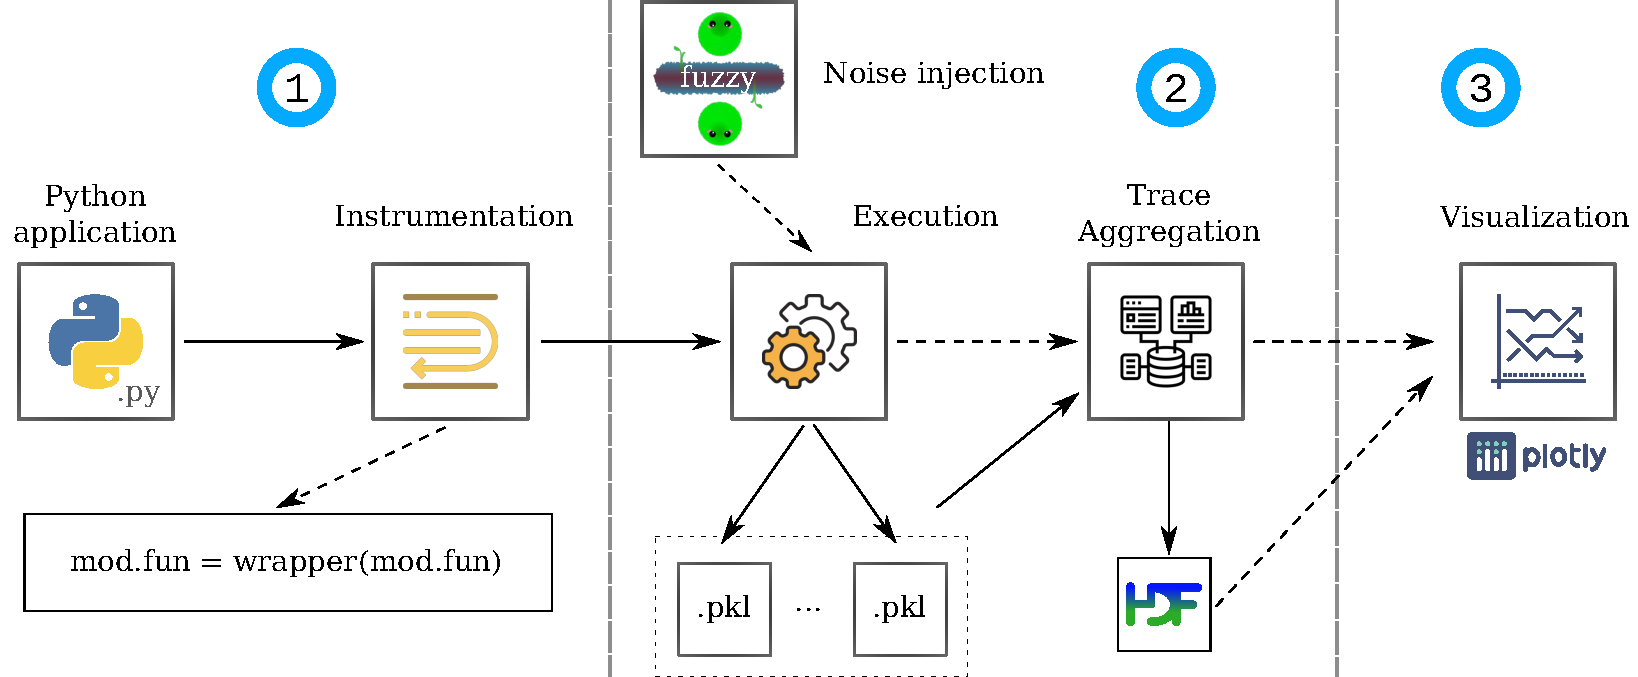
\includegraphics[width=\linewidth]{figure/workflow.pdf}
    \caption{Pytracer workflow}
    \label{fig:workflow}
\end{figure}

\subsection{Python code instrumentation}

%\tristan{``Instrumentation" should appear in Figure 1}


\pytracer dynamically instruments Python modules
without requiring source code modifications in the application.
To do so, it creates a new, instrumented version of each module that preserves its original attributes so that the original application can transparently use it.
By default, \pytracer instruments all the attributes
in a given module except the special ones of the form \texttt{\_\_*\_\_}.
However, some attributes are not writable; in this case, \pytracer preservers the original attributes and warns the user. The user can also restrict the list of traced attributes through
an inclusion/exclusion mechanism. The main advantage of this instrumentation approach is the lack of required modification in the application source code, in contrast with decorator-based approaches, which is scalable and useful in read-only environments such as Singularity containers or HPC clusters.


\subsubsection{Intercepting module import}

Python loads modules through an import mechanism triggered by the \texttt{import} keyword, using two objects: \texttt{finders} and \texttt{loaders}.
The \texttt{finder} is responsible for finding the package (or 
namespace\footnote{Python distinguishes between \texttt{regular} and \texttt{namespace} packages.
A regular package is a directory that contains a \_\_init\_\_.py file and potentially subdirectories (sub-packages) 
that contain themselves a \texttt{\_\_init\_\_.py} file and so on recursively. 
The package hierarchy follows those of the directory. 
Namespace packages introduced in Python 3.3 (\href{https://www.python.org/dev/peps/pep-0420/}{PEP 420}) do not contain an
\_\_init\_\_.py file and allow for flexible directory structures. Hence, parts of the package can be located in zip files, on the network, or in separated directories. There are no functional differences between both types of packages.}) from its fully qualified name, whether it is located on the local storage, such as standard packages installed through the pip package manager, or on a distant server.
\texttt{Finders} do not load the modules; they return a specification (\texttt{spec} object) encapsulating 
information on where to find it and how to load it.
The \texttt{loader} creates and initializes a module object, filling the import-related attributes 
such as \texttt{\_\_spec\_\_}. 
Then, the \texttt{loader} executes the module and populates its namespace. Finally, the module is bound to its import name in the \texttt{sys.modules} dictionary.


Python supports custom \texttt{finder} classes, registered in the \texttt{sys.meta\_path} list.
When Python encounters an \texttt{import} statement, it first looks for a binding in the \texttt{sys.modules}
and then iterates over the \texttt{finder} classes in \texttt{sys.meta\_path} until it finds the module to import. \pytracer adds a custom \texttt{finder} class at the head of the list that intercepts
the module import and creates the module with a custom \texttt{loader} class.

\pytracer's \texttt{loader} class first loads the original module, then copies it as a new instance of the \texttt{ModuleType} class. It then calls the appropriate instrumentation function for each module attribute depending on its type (function, class, or instances). Then, \pytracer replaces the original module with its instrumented counterpart in the \texttt{sys.modules} map once it has instrument all the attributes. Hence, the calling convention remains unchanged, and the application will transparently call the instrumented module. Finally, Pytracer updates all existing references to the original module, such as the ones in \texttt{\_\_globals\_\_} function attributes that contain references to internal function objects. 

% \tristan{is the non-instrumented version ever added to sys.modules? If so, could this lead to race conditions? If not, replace with ``adds the instrumented module to the sys.modules map"}. 
% \Yohan{Yes, it replaces the original module. You can't have a race-condition since sys.modules is a dict with only one value for a given key. The trick is that the wrapped module keeps a reference to the original module, it's just that this reference is invisible for the others object since it's not in sys.modules and globals. By the way, Pytracer needs to update all possible references that original objects may hold, like functions in \_\_dict\_\_ attributes or locals references in \_\_globals\_\_ for example.}

% \pytracer intercepts the modules loaded with the \texttt{Finder} and \texttt{Loader} mechanisms \tristan{is it restrictive? Are there other mechanisms?}.
% The Finder searches the loader of a module that is being imported while the 
% Loader loads and initializes the module. \pytracer adds \tristan{overrides?} a new Finder and Loader on top of the default ones
% to intercept imports and to instrument modules selected by the user. This mechanism allows returning 
% the original module in the instrumentation code and returning the instrumented module in the targeted application
% without modifying its actual code.

\subsubsection{Instrumenting module functions}

For each function, \pytracer's \texttt{loader} class creates a wrapper function, dynamically compiles it with the compile builtin function, and substitutes it for the original module function. This simple technique
cannot be applied to callable class instances, i.e., class instances that have the \texttt{\_\_call\_\_} attribute but are not of the \texttt{FunctionType} type. Indeed, applying the wrapper technique would 1) modify the type of the class instance to \texttt{FunctionType}, which could cause syntactic and semantic bugs, and 2) mask class attributes, leading to \texttt{AttributeError} exceptions.
To overcome this issue, \pytracer overrides the \texttt{\_\_call\_\_} attribute with the wrapper function when possible. When the \texttt{\_\_call\_\_} attribute is not writable,  Pytracer does not instrument the class and returns a warning. 
Listings~\ref{fig:wrapper_creation} and~\ref{fig:generic_wrapper} show \pytracer's wrapper creation function.

% \tristan{add docstrings to all Python code examples and clarify captions accordingly: you don't need to explain the meaning of each attribute in the caption if it's in the docstring. The caption can focus on the main functionality, reusing the text currently in 3.1.5.}
% \Yohan{TODO}

% Listing~\ref{fig:wrapper_creation} shows how functions are instrumented.
% This function takes as inputs the information about the function to instrument (module name and full qualified name),
% the function itself, and the actual name of the function. It then creates a wrapper around the actual wrapper
% (\texttt{generic\_wrapper}) that will save the values in trace files. Instead of passing the function, we pass the function's identifier, which is a unique 64-bits integer that references each Python object. This identifier is available
% with the \texttt{id} builtin function. it allows to get rid of aliases and to avoid instrumenting functions twice.  \tristan{Summarize this paragraph in the figure caption}

% Listing~\ref{fig:generic_wrapper} shows what the instrumented code does. 
% It first unpacks the function's information to get the function's identifier to retrieve the original function.
% Then arguments are bound by creating a mapping from positional and keyword arguments to parameters, avoiding conflicts and mispositioning. It also allows getting names of arguments for the visualization.
% Once bound, the \texttt{inputs} function dumps the arguments in the pickle file.
% Finally, Pytracer calls the function with the correct arguments, dumps the result, and returns it. \tristan{Summarize this paragraph in the figure caption}

%
% we can employ a case by case strategy depending on the class (i.e. numpy ufunc) or simply ignore
% the instrumentation and let the original one.
% \tristan{add a sentence to explain how callable instances are instrumented}




\begin{listing}
    \centering
\begin{lstlisting}[language=Python,style=customPython]
def get_wrapper_function(module, qualname, name, function):
    """Returns the instrumented function as a string.
    This string will be compiled with the compile builtin function
    
    Parameters:
        module: Name of the function module
        qualname: Qualified name of the function
        name: Name of the function
        function: Python object function
        
    Returns:
        wrapper_code: The code source of the wrapper
    """
    function_id = id(function)
    info = (function_id, function_module, function_qualified_name)
    wrapper_code = f"""
    def {function_wrapper_name}(*args, **kwargs):
        return generic_wrapper({info},*args,**kwargs)"""
    return wrapper_code
\end{lstlisting}
    \caption{Function to create the instrumented version of a function.
    \pytracer uses the identifier of the function instead of the 
    actual function to get rid of aliases and duplicated instrumentations.}
    \label{fig:wrapper_creation}
\end{listing}


\begin{listing}
    \centering
\begin{lstlisting}[language=Python,style=customPython,]
def generic_wrapper(self, info, *args, **kwargs):
    """Generic wrapper dumping inputs and outputs of the wrapped function.
    The id_dict dict keeps a mapping between the original function identifier
    and itself. Arguments are binded to avoid mispositioning.
    Returns the actual output of the wrapped function.
    
    Parameters:
        info: Tuple with the function's id, function's module and function's name
        *args: Positional calling arguments
        **kwargs: Keyword calling arguments
    
    Returns:
        outputs: Outputs of the wrapped function
    """
    fid, fmodule, fname = info
    function = original_function_cache.id_dict[fid]
    bind = Binding(function, *args, **kwargs)
    stack = self.backtrace()
    time = elements()
    self.inputs(time=time,
                module_name=fmodule,
                function_name=fname,
                function=function,
                args=bind.arguments,
                backtrace=stack)
    outputs = function(*bind.args, **bind.kwargs)
    self.outputs(time=time,
                 module_name=fmodule,
                 function_name=fname,
                 function=function,
                 args=outputs,
                 backtrace=stack)
    return outputs
\end{lstlisting}
    \caption{\pytracer's wrapper function that dumps
    the inputs and outputs of the wrapped function.
    \pytracer binds arguments to the function signature to avoid
    mispositioning and to have actual names for the visualization.
    The wrapper returns the actual output.
    }
    \label{fig:generic_wrapper}
\end{listing}


\subsubsection{Instrumenting classes}

\pytracer instruments classes by wrapping their callable attributes as described previously. 
This instrumentation preserves class types, avoiding type mismatches in the instrumented application.
However, some classes, in particular base types and NumPy's universal functions (\texttt{ufuncs}), contain read-only attributes that cannot be instrumented. 
By default, \pytracer returns a warning when it encounters such classes. 

\subsubsection{Instrumenting instances}

Pytracer automatically instruments the instances since it instruments the classes, but it cannot instruments or instantiates some classes like \texttt{ufunc}, although their instrumentation is desirable given their pervasiveness in scientific computing. 
Indeed, NumPy's \texttt{ufuncs} are vectorized element-wise operators that apply to multidimensional arrays, 
including the set of elementary mathematical functions.
In particular, all the element-wise elementary mathematical functions are \texttt{ufuncs}.  
To increase performance, \texttt{ufuncs} are implemented in C, which prevents their instantiation.

To overcome this issue, \pytracer wraps the instances into a transparent wrap class (\texttt{twc}) that overloads
1) the \texttt{\_\_getattribute\_\_} that is called when one is accessing an instance's attribute.
The \texttt{twc} returns the queried attribute of the instance instead of returning its attributes, allowing transparent access to the instance. 2) the \texttt{\_\_call\_\_} functions that is called when one 
is calling the function (through the () operator). The \texttt{twc} calls the \texttt{generic\_wrapper} to saves 
inputs and outputs as for classical functions. Finally, \pytracer overloads the \texttt{type} built-in function
to preserve the type of the wrapped instance.

\subsubsection{Instrumenting iterators}

In functional programming, iterators traverse containers lazily, meaning that the next element in the sequence is only computed when the application uses it. This technique allows for the manipulation of virtually infinite sequences with finite memory. However, it implies that no complete mapping of the container returned by an iterator exists in memory since the application computes each element on the fly. Therefore, iterators are not serializable and \pytracer cannot save them to output traces. 
A workaround would be to convert iterators into explicit containers and then return a new iterator on the explicit container. However, this would increase the memory footprint significantly. \pytracer therefore does not instrument iterators.

% \begin{listing}
% \begin{minipage}[t]{0.4\linewidth}
%     \begin{lstlisting}[language=Python,style=customPython]
% >>> import numpy as np
% >>> x = np.array(range(10))
% >>> index = np.array([1,-1],dtype=int)
% >>> x[index]
% >>> array([1, 9])
%     \end{lstlisting}
% \end{minipage}
% \begin{minipage}[t]{0.4\linewidth}
%     \begin{lstlisting}[language=Python,style=customPython]
% >>> import numpy as np
% >>> x = np.array(range(10))
% >>> index = np.array([1,-1], dtype=object)
% >>> x[index]
% Traceback (most recent call last):
%   File "<stdin>", line 1, in <module>
% IndexError: arrays used as indices must be of integer (or boolean) type
%     \end{lstlisting}
% \end{minipage}
% \caption{Illustration of the issue of using \texttt{frompyfunc} function to convert function to \texttt{ufunc}. Left: original code. Right: instrumented code. 
% \tristan{This needs more explanation: where is the ufunc, what is the type returned by the original ufunc, and why does it crash in the instrumented version.} \Yohan{TODO}}
%     \label{fig:numpy_array_index_issue}
% \end{listing}

\subsection{Detecting numerical instabilities}

\pytracer detects numerical instabilities by computing summary statistics across multiple executions perturbed with numerical noise. While \pytracer's instrumentation, trace aggregation, and visualization work with various types of numerical noise, we experimented primarily with Monte-Carlo Arithmetic (MCA) as it is an accurate model for floating-point errors.

\subsubsection{Noise injection}
\label{sec:fuzzy}


We enable MCA in Python programs via Verificarlo~\cite{verificarlo}, a clang-based compiler~\cite{lattner2008llvm} that replaces floating-point operations by a generic call to a configurable floating-point model. Several floating-point models, also called backends, are available~\cite{chatelain2019automatic,chatelain2019outils}.
We leverage the ``fuzzy"~\cite{kiar2020comparing} environment, a collection of software tools recompiled with Verificarlo. In particular, fuzzy provides MCA-instrumented versions of the Python interpreter as well as of the BLAS, LAPACK, NumPy, SciPy, and scikit-learn libraries, which enables MCA for a wide range of existing scientific Python programs. Fuzzy is available in Verificarlo's GitHub organization at \href{https://github.com/verificarlo/fuzzy}{\url{github.com/verificarlo/fuzzy}}.

% As the time of writing this article, fuzzy provides 5 levels of instrumentation (each level N including the lower levels):
% \begin{enumerate}
%     \item BLAS + LAPACK
%     \item Python interpreter
%     \item Numpy
%     \item SciPy
%     \item Scikit-learn
% \end{enumerate}

\subsubsection{Trace format}

\pytracer stores traces in the pickle format, a compressed binary Python format to serialize Python objects.
The main advantages of the pickle format compared to other serialization approaches such as marshal or JSON are its ability to serialize most Python objects and its native compression.  In addition, pickle writes Python objects sequentially, which preserves the temporal ordering required by subsequent trace analyses.

Traces record numerical values at the granularity of a function. When the application invokes a function, \pytracer saves a call input object containing contextual information (function's name, module's function, stacktrace) and the values of the function arguments. When the function returns, \pytracer saves a similar call output object containing the returned value. 


\subsubsection{Trace aggregation}

Once traces are available, \pytracer sequentially parses them and computes the mean, standard deviation, and the number of significant digits (computed using Equation~\ref{eq:sig-digits}) of all saved values. Pytracer saves these summary statistics in an HDF5 file, a hierarchical format that facilitates browsing during the visualization. This operation critically relies on the ordering of call input and output objects in the traces. Furthermore, it assumes that the application is deterministic, and in particular, assumes it is single-threaded and that the control flow does not depend on a random state. 
% Techniques to overcome this limitation are discussed in the discussion section.

\begin{figure}
    \centering
    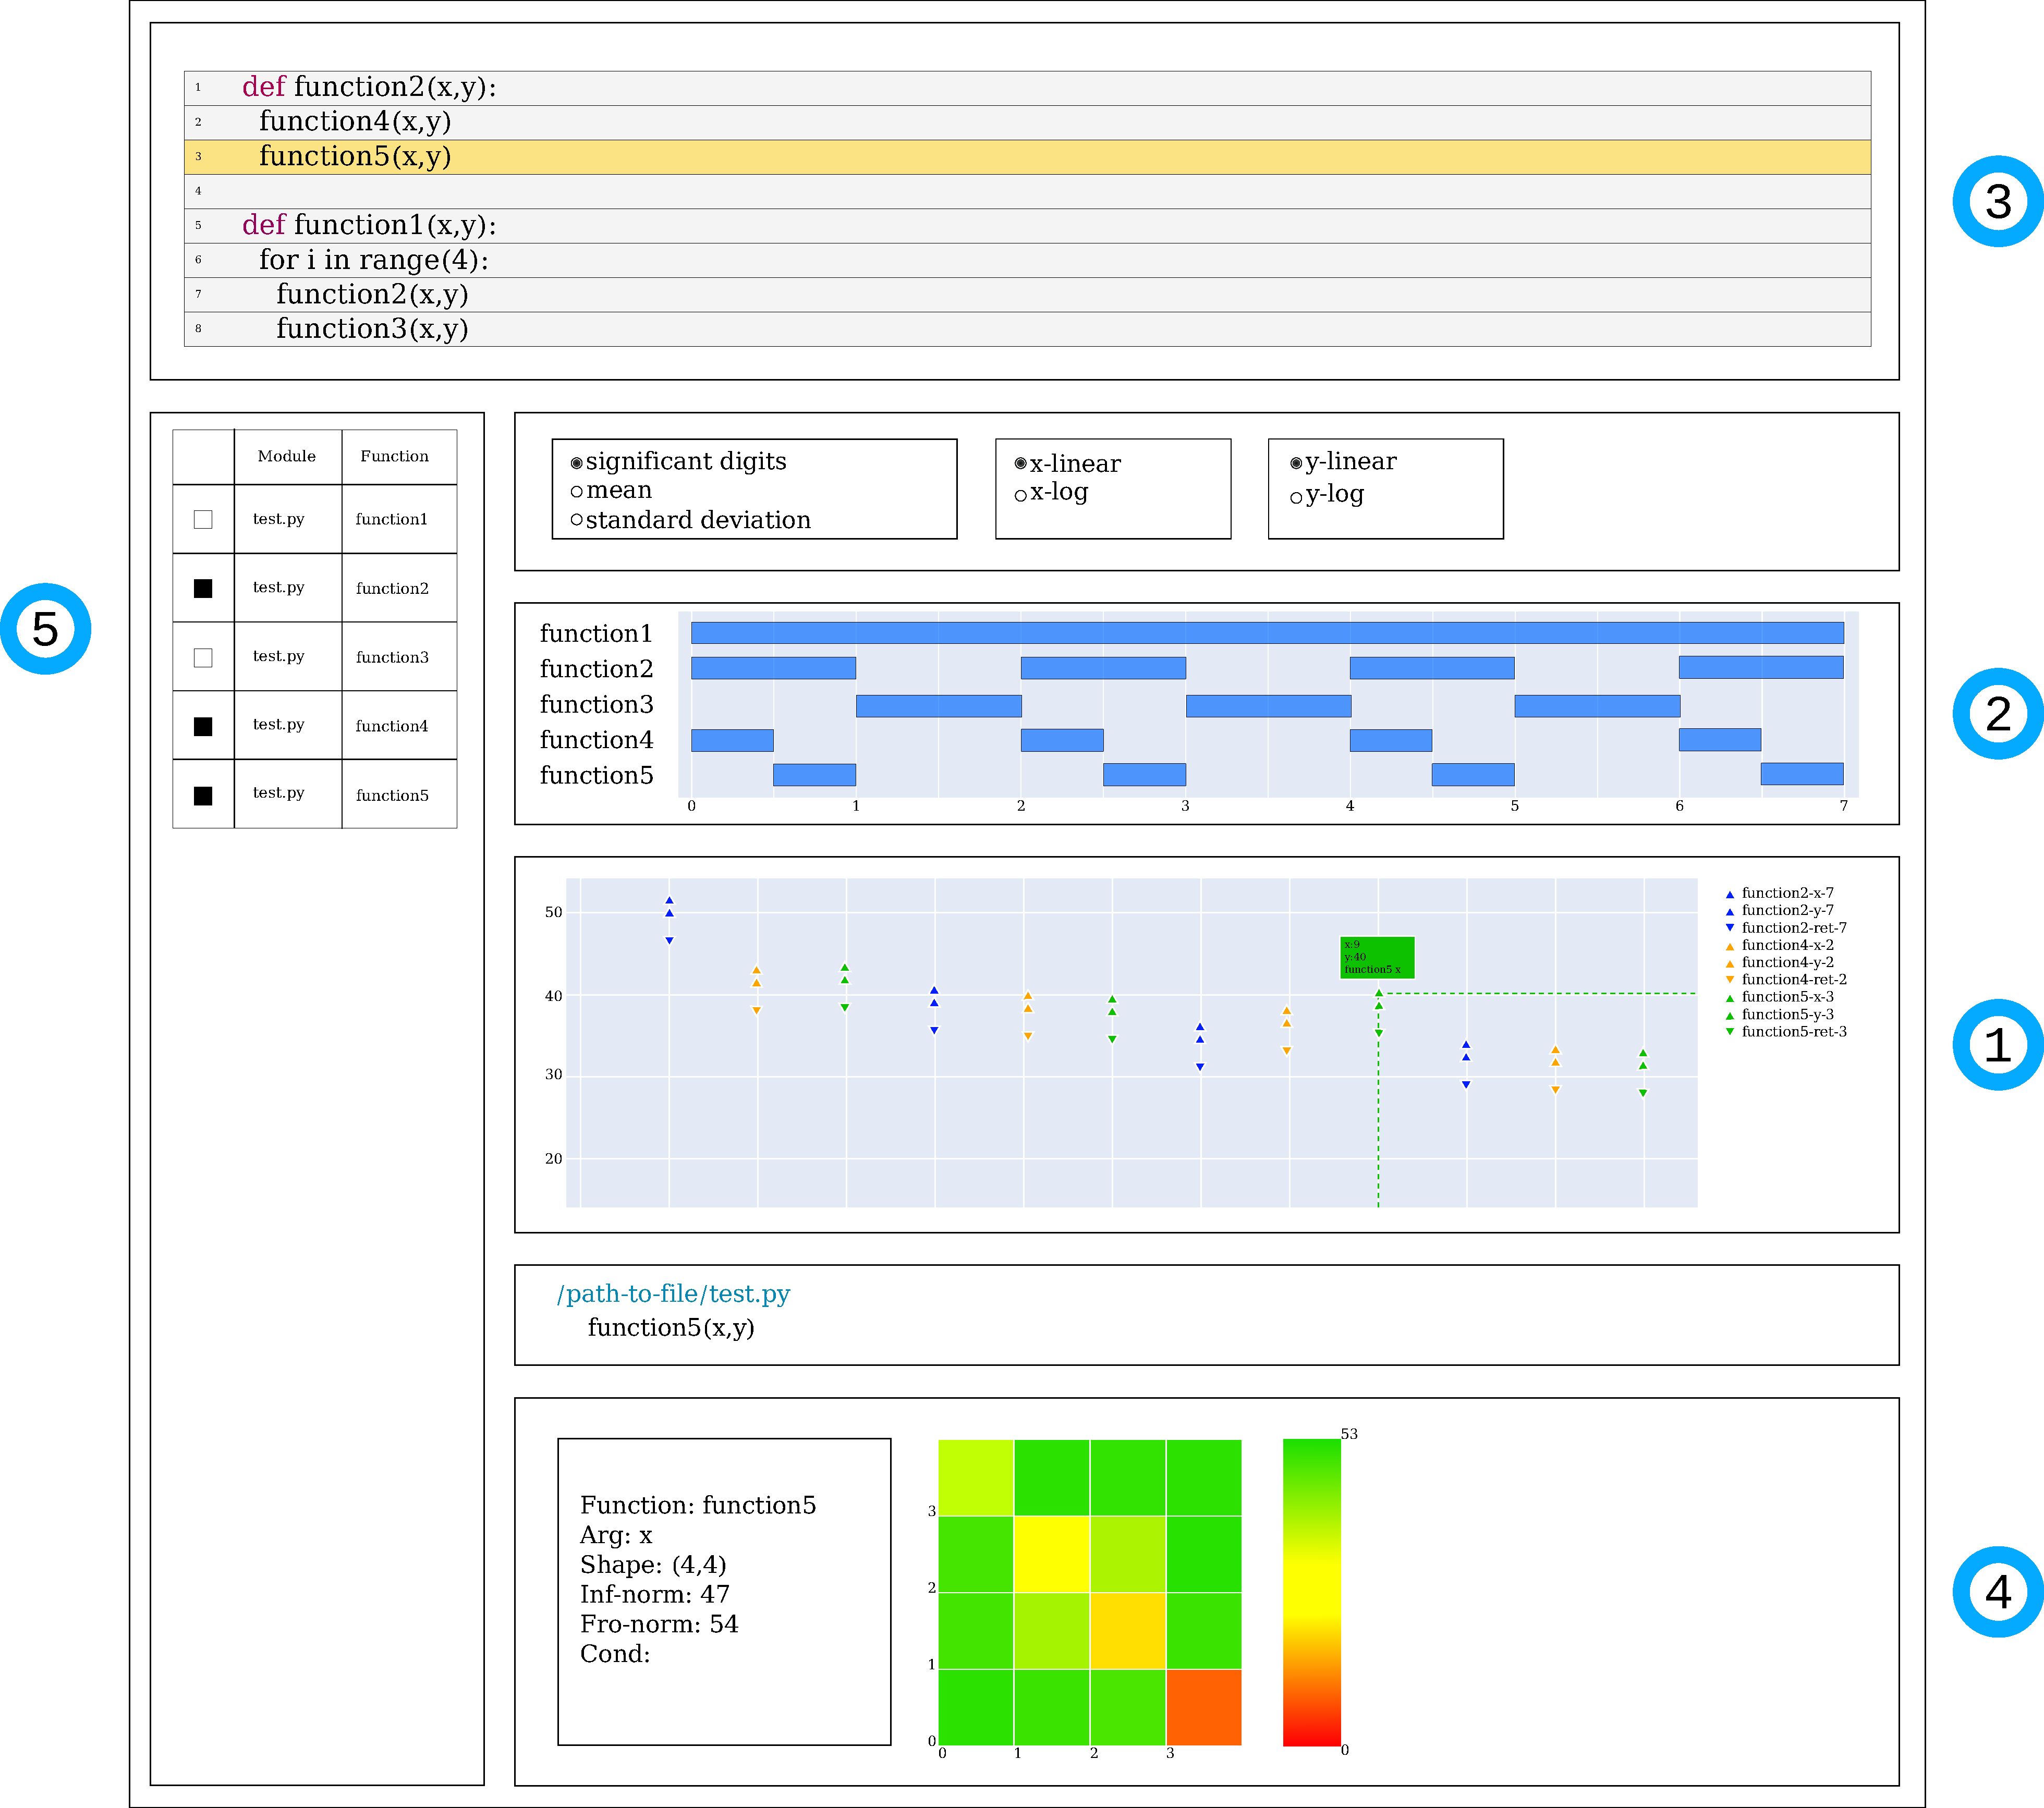
\includegraphics[width=\textwidth]{figure/pytracer_layout.pdf}
    \caption{Pytracer visualization layout.}
    \label{fig:visu-layout}
\end{figure}


To aggregate traces, \pytracer successively unpickles call objects in each trace, checks
that the call objects refer to the same function and stacktrace, and terminates the parsing otherwise.
For each matching call object, \pytracer stores function arguments or returned values in a NumPy array to compute statistics. 
For compound objects such as tuples, dictionaries, or objects, it recursively parses the fields until finding
numeric types or NumPy arrays of numeric types.

\subsection{Interactive visualization}
The third main component of \pytracer is its interactive trace visualizer built with Plotly Dash~\cite{plotly}, a Python framework for web visualization.
Plotly Dash abstracts the low-level details of web applications in a highly customizable development interface allowing to offload heavy computations to a server. 
Figure~\ref{fig:visu-layout} presents the general layout of the \pytracer visualizer, divided into five sub-components:
\begin{enumerate}
 \item Timeline view: This view displays the values of each input and output for a given function at a given invocation. By default, \pytracer shows the number of significant digits computed across the traces, but the user can switch to the mean or the standard deviation. The visualizer uses an upper triangle for inputs and a down triangle to differentiate inputs from outputs. \pytracer internally represents all values as NumPy arrays.    In the case of non-scalar values or types that cannot be trivially cast into NumPy arrays, \pytracer splits the value into several variables. Hence, \pytracer will transform a class containing $n$ floating-point parameters into $n$ variables. Each variable is prefixed with the original value and postfixed with the name of the parameter. 
    Finally, for non-scalar values (vectors or matrices), \pytracer shows the average elements for non-scalar values (like vectors or matrices). non-scalar values can be inspected with the Zoom view (see below).
 \item Gantt chart view: This view displays the call graph as a Gantt chart representing the instrumented functions. Each function call is represented with a bar starting and ending at the function call and return.
    The caller/callee relation is then determined by looking at the time overlaps.
    For example, in the figure, \texttt{function1} calls \texttt{function2} that itself calls \texttt{function4} and \texttt{function5}. 
    This view provides insights on the calling context for each function since different parents functions can call the same function, which may influence numerical stability. 
 \item  Source code view: This view displays the source code file of the variable hovered in the timeline view. 
 \item Zoom view: This view allows closely examine non-scalar values, which is helpful to see local differences that might be masked by the averaging done in the timeline view. For example, a matrix can have instabilities around its diagonal but not in other regions.
    The visualizer also provides metrics about the value, such as the array shape, infinite norm, or condition number.
\item  Functions list view: This view allows the user to select the functions to plot in the timeline view.
\end{enumerate}

\section{Numerical evaluations}

We evaluated \pytracer on widely-used Python libraries, namely: SciPy, the main library for scientific computing in Python; scikit-learn, a reference machine-learning framework; PyAFQ, a neuroimaging analysis toolbox.
For SciPy and scikit-learn, we traced each application five times, having activated MCA in the Python interpreter, BLAS, LAPACK, NumPy, SciPy, and scikit-learn. We repeated the experiment with two MCA modes, Random Rounding (RR) and Full MCA, resulting in 2 experiments for each application. We used the default virtual precision in Verificarlo, namely 24 bits for single-precision floating-point values and 53 bits for double-precision values, which simulates machine error. For each library, we executed the software tests provided in their GitHub repositories.

\subsection{Results overview}

Tables~\ref{tab:pytracer_scipy_results_summary} and~\ref{tab:pytracer_sklearn_results_summary} summarize 
\pytracer's outcome on SciPy and scikit-learn tests.
Each table reports on the tracing and trace aggregation steps with three possible outcomes: green for success, red for numerical error in the application, and orange for errors in the fuzzy noise injection. Overall, the tracing and parsing of SciPy and scikit-learn tests in Random Rounding mode was entirely successful (tracing and parsing steps) for 32/40 tests. The remaining tests failed due to numerical errors in the libraries, which we discuss hereafter. The instrumentation with Full MCA is more invasive and reduced the number of successful executions to 13/40.

\begin{table}[]
    \centering
    \begin{tabular}{|ll|c|c|c|c|}
    \hline
    \multicolumn{2}{|c}{ \multirow{2}{*}{Application} } & \multicolumn{2}{|c|}{RR} & \multicolumn{2}{c|}{Full MCA} \\
    \cline{3-6}
    & & trace & parse & trace & parse  \\
    \hline
    %        &               RR                 &                 MCA               \\
    %        &  numpy         &   no numpy      &      numpy      &     no numpy    \\
    %        & run   & parse  &  run   &  parse &  run   & parse  & run    & parse  \\
    
    \multicolumn{1}{|c|}{ \multirow{3}{2em}{ \rotatebox{90}{FFT} } }
    & discrete\_cosine\_transform &  \valid & \valid & \warn & \cross \\ 
    \multicolumn{1}{|c|}{} & fft\_1D & \valid & \valid& \warn & \cross \\
    \multicolumn{1}{|c|}{} & fft\_2D & \valid & \valid & \valid & \valid \\
    \hline 
    \multicolumn{1}{|c|}{  \multirow{5}{2em}{ \rotatebox{90}{Interpolation} } }
    & interpolation\_1D & \valid & \valid & \warn & \cross  \\
    \multicolumn{1}{|c|}{} & multivariate\_data & \valid & \valid & \warn & \cross \\
     \multicolumn{1}{|c|}{} & bspline  & \valid & \valid & \valid & \valid \\
     \multicolumn{1}{|c|}{} & spline\_1D & \valid & \cross & \warn & \cross \\
     \multicolumn{1}{|c|}{} & spline\_2D & \valid & \valid & \warn & \cross \\
    \hline
     \multicolumn{1}{|c|}{ \multirow{12}{2em}{ \rotatebox{90}{Optimization} } }
    & broyden\_fletcher\_goldfarb\_shanno & \valid & \valid & \valid & \valid \\
     \multicolumn{1}{|c|}{} & global\_optimization & \valid & \cross  & \warn & \cross \\
    \multicolumn{1}{|c|}{}  & slsqp & \valid & \valid  & \valid & \valid \\
     \multicolumn{1}{|c|}{} & least\_square\_minimization & \valid & \valid  & \warn & \cross \\
     \multicolumn{1}{|c|}{} & nelder\_mead\_simplex  & \valid & \valid  & \valid & \valid \\
     \multicolumn{1}{|c|}{} & newton\_conjugate\_gradient  & \valid & \valid  & \valid & \cross \\
     \multicolumn{1}{|c|}{} & root\_findings  & \valid & \cross & \warn & \cross \\
    \multicolumn{1}{|c|}{}  & root\_finding\_large & \valid & \cross  & \valid & \cross \\
     \multicolumn{1}{|c|}{} & root\_finding\_large\_preconditionned & \valid & \cross & \valid & \cross \\
    \multicolumn{1}{|c|}{}  & trust\_region\_exact& \valid & \valid  & \valid & \valid \\
     \multicolumn{1}{|c|}{} & trust\_region\_truncated\_generalized\_lanczos & \valid & \valid & \valid & \valid \\
    \multicolumn{1}{|c|}{}  & trust\_region\_newton\_conjugate\_gradient & \valid & \valid & \valid & \valid \\
    \hline
    \end{tabular}
    \caption{\pytracer execution summary on SciPy tests.\\RR: Random Rounding. trace: outcome of \pytracer tracing, parse: outcome of \pytracer trace parsing and aggregation.  \valid: successful run, \warn: error in fuzzy noise injection, \cross: numerical error or divergent traces.}
    \label{tab:pytracer_scipy_results_summary}
\end{table}

\begin{table}[]
    \centering
    \begin{tabular}{|c|c|c|c|c|}
    \hline
    \multirow{2}{5em}{Application} & \multicolumn{2}{c|}{RR} & \multicolumn{2}{c|}{MCA} \\\cline{2-5}
                                & trace & parse &  trace & parse \\
    \hline
    %        &               RR                 &                 MCA               \\
    %        &  numpy         &   no numpy      &      numpy      &     no numpy    \\
    %        & run   & parse  &  run   &  parse &  run   & parse  & run    & parse  \\
    Adaboost & \valid & \valid  & \warn & \cross \\
    Bayesian Ridge Regression  & \valid & \valid  & \cross & \cross \\
    Online classifier comparison & \valid & \valid  & \warn & \cross  \\
    K-Means Clustering  & \valid & \valid  & \valid & \cross \\
    Covariance estimation  & \valid & \cross  & \warn & \cross \\
    Decision Tree Regression & \valid & \valid  & \valid & \valid \\
    Digits Classification  & \valid & \valid  & \warn & \cross \\
    Face Recognition  & \cross & \valid  & \warn & \cross \\
    L1 Penalty  & \valid & \valid  & \valid & \valid \\
    Lasso and elastic net  & \valid & \valid  & \warn & \cross \\
    Separating hyperplan  & \valid & \valid  & \valid & \cross \\
    MNIST classification  & \valid & \valid  & \warn & \valid \\
    Multitask Lasso  & \valid & \valid  & \warn & \valid \\
    Orthogonal matching & \valid & \valid  & \valid & \valid \\
    PCA decomposition  & \valid & \valid  & \valid & \valid \\
    Robust Linear Regression  & \valid & \valid  & \warn & \cross \\
    Segmentation toy  & \valid & \valid  & \warn & \cross \\
    SVM  & \valid & \valid  & \valid & \cross \\
    Tomography  & \valid & \cross  & \warn & \cross \\
    Weighted samples  & \valid & \valid  & \valid & \cross \\
    \hline
    \end{tabular}
    \caption{\pytracer execution summary on Scikit-learn tests. \\RR: Random Rounding. trace: outcome of \pytracer tracing, parse: outcome of \pytracer trace parsing and aggregation. \valid: successful run, \warn: error in fuzzy noise injection, \cross: numerical error or divergent traces.}
    \label{tab:pytracer_sklearn_results_summary}
\end{table}



\subsubsection{Effect of MCA modes}
\label{sec:impact_mca_modes}
Random Rounding perturbs only the result of a floating-point operation, while Full MCA mode perturbs both the inputs and the operation's result. 
Therefore, full MCA mode may trigger catastrophic cancellations while Random Rounding only introduces round-off errors which generally have a lesser impact.
Moreover, Random Rounding preserves exact operations, i.e., operations where the result can be exactly represented on the virtual precision, while Full MCA does not.

\pytracer can only aggregate traces obtained from the same control flow path. In particular, program branches triggered by an unstable floating-point comparison lead to different control flows and result in parsing errors. 
For example, comparing a residual error to a strict threshold in an iterative scheme or comparing the distance between two points generally results in unstable branches. 
With Full MCA, even exact values such as integers represented with floating-point values are perturbed, leading to many execution failures. For instance,  the \texttt{fft1} test from SciPy raised an \texttt{ValueError: operands could not be broadcast together with shapes (601,) (600,)} error due to an array shape mismatch. A closer inspection showed that one of the arrays involved in the error is created with the NumPy function \texttt{linspace} that itself calls function \texttt{arange} (Listing~\ref{fig:pyarray_range_code}). As can be seen in lines  3174-3178, the array size is stored in a floating-point value which will therefore be perturbed in Full MCA mode, as shown in Table~\ref{tab:mca_result_linspace}, resulting in array sizes that fluctuate
between N and N+1. 
It is worth noting that 78\% of execution issues encountered in Full MCA mode without \texttt{ufunc} instrumentation
are due to this type of ``typing" errors. While they do not lead to any numerical issue, such typing errors should still be fixed to preserve code quality. We provide solutions to help MCA better work with those cases in the discussion section.

\tristan{Check this last sentence, we need to provide some sort of recommendations}. \tristan{how about opening a PR in numpy to fix this error?}
\Yohan{For this case, they use the math.ceil to correctly round the number, I think the fix is more on the MCA side to
correctly handle exact number than on the NumPy side.}


% \begin{figure}
%     \begin{lstlisting}[language=Python,style=customPython,numbers=left, firstnumber=11]
% # Number of sample points
% N = 600
% # sample spacing
% T = 1.0 / 800.0
% x = np.linspace(0.0, N*T, N, endpoint=False)
% y = np.sin(50.0 * 2.0*np.pi*x) + 0.5*np.sin(80.0 * 2.0*np.pi*x)
% yf = fft(y)
% w = blackman(N)
% ywf = fft(y*w)
%     \end{lstlisting}
%     \label{fig:fft1_code}
% \caption{Code snippet from \texttt{fft\_1D} illustrating issue arising when using Full MCA mode.
% Line 19 raises \texttt{ValueError: operands could not be broadcast together with shapes (601,) (600,)} since
% arrays \texttt{y} and \texttt{w} do not have the same shape. This is due to random errors introduces by 
% Full MCA mode in the \texttt{linspace} function.
% }
% \end{figure}

% \begin{figure}
%     \begin{lstlisting}[language=Python,style=customPython,numbers=left, firstnumber=1, mathescape=true]
% def linspace(start, stop, num=50, endpoint=True, retstep=False, dtype=None,
%              axis=0):
%     num = operator.index(num) // 3 $\lstsetnumber{\ldots}$
%     ...$\lstresetnumber\setcounter{lstnumber}{5}$
%     div = (num - 1) if endpoint else num // 6  $\lstsetnumber{\ldots}$
%     ...$\lstresetnumber\setcounter{lstnumber}{13}$
%     delta = stop - start // 14
%     y = _nx.arange(0, num, dtype=dt).reshape((-1,) + (1,) * ndim(delta)) // 15
%     \end{lstlisting}
%     \label{fig:linspace_code}
% \caption{Code snippet from \texttt{linspace} function from numpy package. 
%     It uses the \textit{arange} function implemented as a Cython function (fig.~\ref{fig:pyarray_range_code}) to create the array. 
% }
% \end{figure}
    

\begin{listing}
    \begin{lstlisting}[language=C,style=customC,numbers=left, firstnumber=3163, mathescape=true]
/*NUMPY_API
  Arange,
*/
NPY_NO_EXPORT PyObject *
PyArray_Arange(double start, double stop, double step /* default 1 */, int type_num) 
{
    npy_intp length; 
    PyArrayObject *range; $\lstsetnumber{\ldots}$
    ...$\lstresetnumber\setcounter{lstnumber}{3173}$
    double delta, tmp_len; $\lstsetnumber{\ldots}$
    ...$\lstresetnumber\setcounter{lstnumber}{3176}$
    delta = stop - start; 
    tmp_len = delta/step; $\lstsetnumber{\ldots}$
    ...$\lstresetnumber\setcounter{lstnumber}{3189}$
        length = _arange_safe_ceil_to_intp(tmp_len); $\lstsetnumber{\ldots}$
    ...$\lstresetnumber\setcounter{lstnumber}{3201}$
    range = (PyArrayObject *)PyArray_New(&PyArray_Type, 1, &length, type_num, $\lstsetnumber{}$
                        NULL, NULL, 0, 0, NULL);
    \end{lstlisting}
\caption{Source code of the \texttt{PyArray\_Range} Cython function called by NumPy function \texttt{linspace} to create an array of equally spaced elements. The temporary array size assigned in line 3178 is stored as a floating-point value and is therefore perturbed in Full MCA mode, leading to differences amplified by the use of ceil rounding at line 3190 and resulting in different array sizes across MCA-perturbed executions. See also Table~\ref{tab:mca_result_linspace}.}
    \label{fig:pyarray_range_code}

\end{listing}

    
\begin{table}[]
    \centering
    \footnotesize
    \begin{tabularx}{{\textwidth}}{cccc>{\centering\arraybackslash}X>{\centering\arraybackslash}X>{\centering\arraybackslash}X}
                \thickhline
    \textbf{Mode}  & \textbf{start} & \textbf{stop} & \textbf{step} & \textbf{delta} & \textbf{tmp\_len} & \textbf{ceil(tmp\_len)}  \\
    \hline
    Exact & 0 & 600  & 1 & 600                             & 600                            & 600             \\
    RR    & 0 & 600  & 1 & 600 $\pm$ 0.0                   & 600 $\pm$ 0.0                  & 600 $\pm$ 0.0   \\
    MCA    & 0 & 600  & 1 & 599.9999999999999 $\pm$ 8e-14  & 600.0 $\pm$ 8e-14 &  600.01 $\pm$ 0.0995\\
            \thickhline

    \end{tabularx}
    \caption{Results obtained through lines 3177-3190 in Listing~\ref{fig:pyarray_range_code}. Contrary to RR mode, Full MCA mode does not preserve exact operations which leads to an array length oscillating between 600 and 601.}
    \label{tab:mca_result_linspace}
\end{table}

\subsubsection{Overall numerical quality}

Table~\ref{tab:pytracer_test_precision_summary} summarizes the precision for main outputs of SciPy and scikit-learn tests. 
We measure the precision in significant bits on the principal output computed by the test by taking the element-wise mean for non-scalar values and, if the test produces many outputs, we take the average value among results. A dash value means that the test produces an error. The numerical quality of obtained results and MCA modes combined vary from 0 to 52, with an average of 44 bits significant. For both modes, we note that only one test failed due to a numerical error (\texttt{face\_recognition} for RR and \textit{Bayesian Ridge Regression} for Full MCA) even though this number is underestimated since Full MCA mode is more intrusive than RR mode and most of the tests produce error caused by the fuzzy noise injection. 

\begin{table}
\small
\begin{subfigure}[t]{.5\linewidth}
    \centering
    \begin{tabular}{|l|c|c|}
    \hline 
    Application & RR & MCA \\
    \hline
    discrete\_cosine\_transform & 52 & 47 \\ 
    fft\_1D & 41 & - \\
    fft\_2D & 52 & 52  \\
    \hline
    interpolation\_1D & 51 & -   \\
    multivariate\_data & 51 & - \\
    bspline  & 10 & 10  \\
    spline\_1D & 52 & 52 \\
    spline\_2D & 10 & - \\
    \hline
    broyden\_fletcher\_goldfarb\_shanno & 48 & 46 \\
    global\_optimization & 17 & - \\
    | SHGO\footnote{Simplicial Homology Global Optimization} & 25 & - \\
    | Dual Annealing & 4 & - \\
    | Differential Evolution & 0 & - \\
    | Basin Hopping & 40 & - \\
    | SHGO Sobol & 45 & - \\
    slsqp & 45 & 44 \\
    least\_square\_minimization & 48 & -  \\
    nelder\_mead\_simplex  & 44 & 42  \\
    newton\_conjugate\_gradient  & 48 & 47 \\
    root\_findings  & 52 & 50 \\
    root\_finding\_large & 29 & 26   \\
    root\_finding\_large\_preconditioned & 42 & 42 \\
    trust\_region\_exact& 48 & 46  \\
    trust\_region\_truncated\_generalized\_lanczos & 48 & 46  \\
    trust\_region\_newton\_conjugate\_gradient & 52 & 47 \\
    \hline
    \end{tabular}
\end{subfigure}
\hspace{1cm}
\begin{subfigure}[t]{.5\linewidth}
    \begin{tabular}{|l|c|c|}
    \hline 
    Application & RR & MCA \\
    \hline
    Adaboost & 48 & - \\
    Bayesian Ridge Regression  & 25 & -  \\
    | $1^{st}$ dataset & nan & - \\
    | $2^{nd}$ dataset & 20 & - \\
    Online classifier comparison & 48 & -  \\
    K-Means Clustering  & 52 & -   \\
    Covariance estimation  & 48 & -   \\
    Decision Tree Regression & 50 & 50  \\
    Digits Classification  & 52 & 52 \\
    Face Recognition  & - & - \\
    L1 Penalty  & - & -   \\
    Lasso and elastic net  & 48 & 47  \\
    Separating hyperplan  & 3 & -  \\
    MNIST classification  & 43 & - \\
    Multitask Lasso  & 50 & 48   \\
    Orthogonal matching & 52 & 52  \\
    PCA decomposition  & 48 & 48   \\
    Robust Linear Regression  & 50 & 48   \\
    | Linear & 48 & 46 \\
    | RANSAC & 50 & 48 \\
    Segmentation toy  & 35 & - \\
    SVM  & 43.5 &  -  \\
    | Non-weighted & 44 & - \\
    | Weighted & 43 & - \\
    Tomography  & - & -  \\
    Weighted samples  & 44 & -   \\
    \hline
    \end{tabular}
\end{subfigure}
    \caption{Summary of tests precision for main outputs of SciPy and scikit-learn tests. Precision is measured in significant bits on the principal output computed by the test.
    For non-scalar values, the element-wise mean is taken. If the test produces many outputs, like when comparing methods, the average value among results is taken.  
    A dash value means that the test produces an error. }
    \label{tab:pytracer_test_precision_summary}
\end{table}


\subsection{SciPy}
\label{sec:scipy_tests}

We tested Pytracer on SciPy~\cite{virtanen2020scipy} examples provided in the tutorial website section.
SciPy is organized in several libraries targeting specific computing domains.
Therefore, we focused on the following packages:
\begin{itemize}
    \item \texttt{fftpack}: Fast Fourier Transform routines.
    \item \texttt{interpolate}: Interpolation and smoothing splines.
    \item \texttt{optimize}: Optimization and root-finding routines.
\end{itemize}

\subsubsection{FFT}

This package has three tests: \texttt{discrete\_cosine\_transform}, \texttt{fft\_1D}, and \texttt{fft\_2D}.
The results for \texttt{discrete\_cosine\_transform},\texttt{fft\_1D} and  \texttt{fft\_2D} show
correct numerical results with 48 significant bits in average. All computations are done with double precision.
We observe that the FFT is stable with noisy inputs. The figures~\ref{fig:fft1D_mean} and~\ref{fig:fft1D_std}
show the mean and standard deviation over the MCA samples respectively. 
The top rows show the domain $z$ and the result fft$(z)$, in the logarithmic scale with the real part in blue and the imaginary part in orange.
The three columns correspond to the FFT computations of: 
\begin{enumerate}
\item $z_1 = \sin(50 . 2\pi . x_i) + \dfrac{1}{2} \sin(80 . 2\pi . x_i),\; x_i = \frac{i}{600},\; i \in [0,600]$
\item $ blackman(400)*z_1$
\item $ z_2= e^{50 . i 2\pi . x_i} + \dfrac{1}{2} e^{-80 . i2\pi .x_i },\; x_i = \frac{i}{800},\; i \in [0,400] $
\end{enumerate}

Top row of figures~\ref{fig:fft1D_mean} and~\ref{fig:fft1D_std} 
shows the mean value of the inputs while the bottom row shows the standard deviation.
The points with low magnitude correspond to inputs near 0, when the input of $\sin$ or 
$\exp$ is close to $k\pi$, $k \in \mathbf{Z}$.
Indeed, since MCA introduces a small noise, the result is not exactly 0.
We can see on the figure~\ref{fig:fft1D_std} that the maximal noise introduced by MCA on the
inputs is of the order of magnitude of $10^{-14}$, two order of magnitude higher than the 
$ulp \simeq 10^-16$ for double precision. 
This small noise introduced can be interpreted as a white noise on the input signal. 
We can see on bottom row of the figure~\ref{fig:fft1D_std} that the frequencies noise is in 
the same order of of magnitude than the magnitude of the inputs noise, which is expected. 
The two pics at 38 and 562 corresponds to the actual frequencies of the input.

\begin{figure}
    \centering
    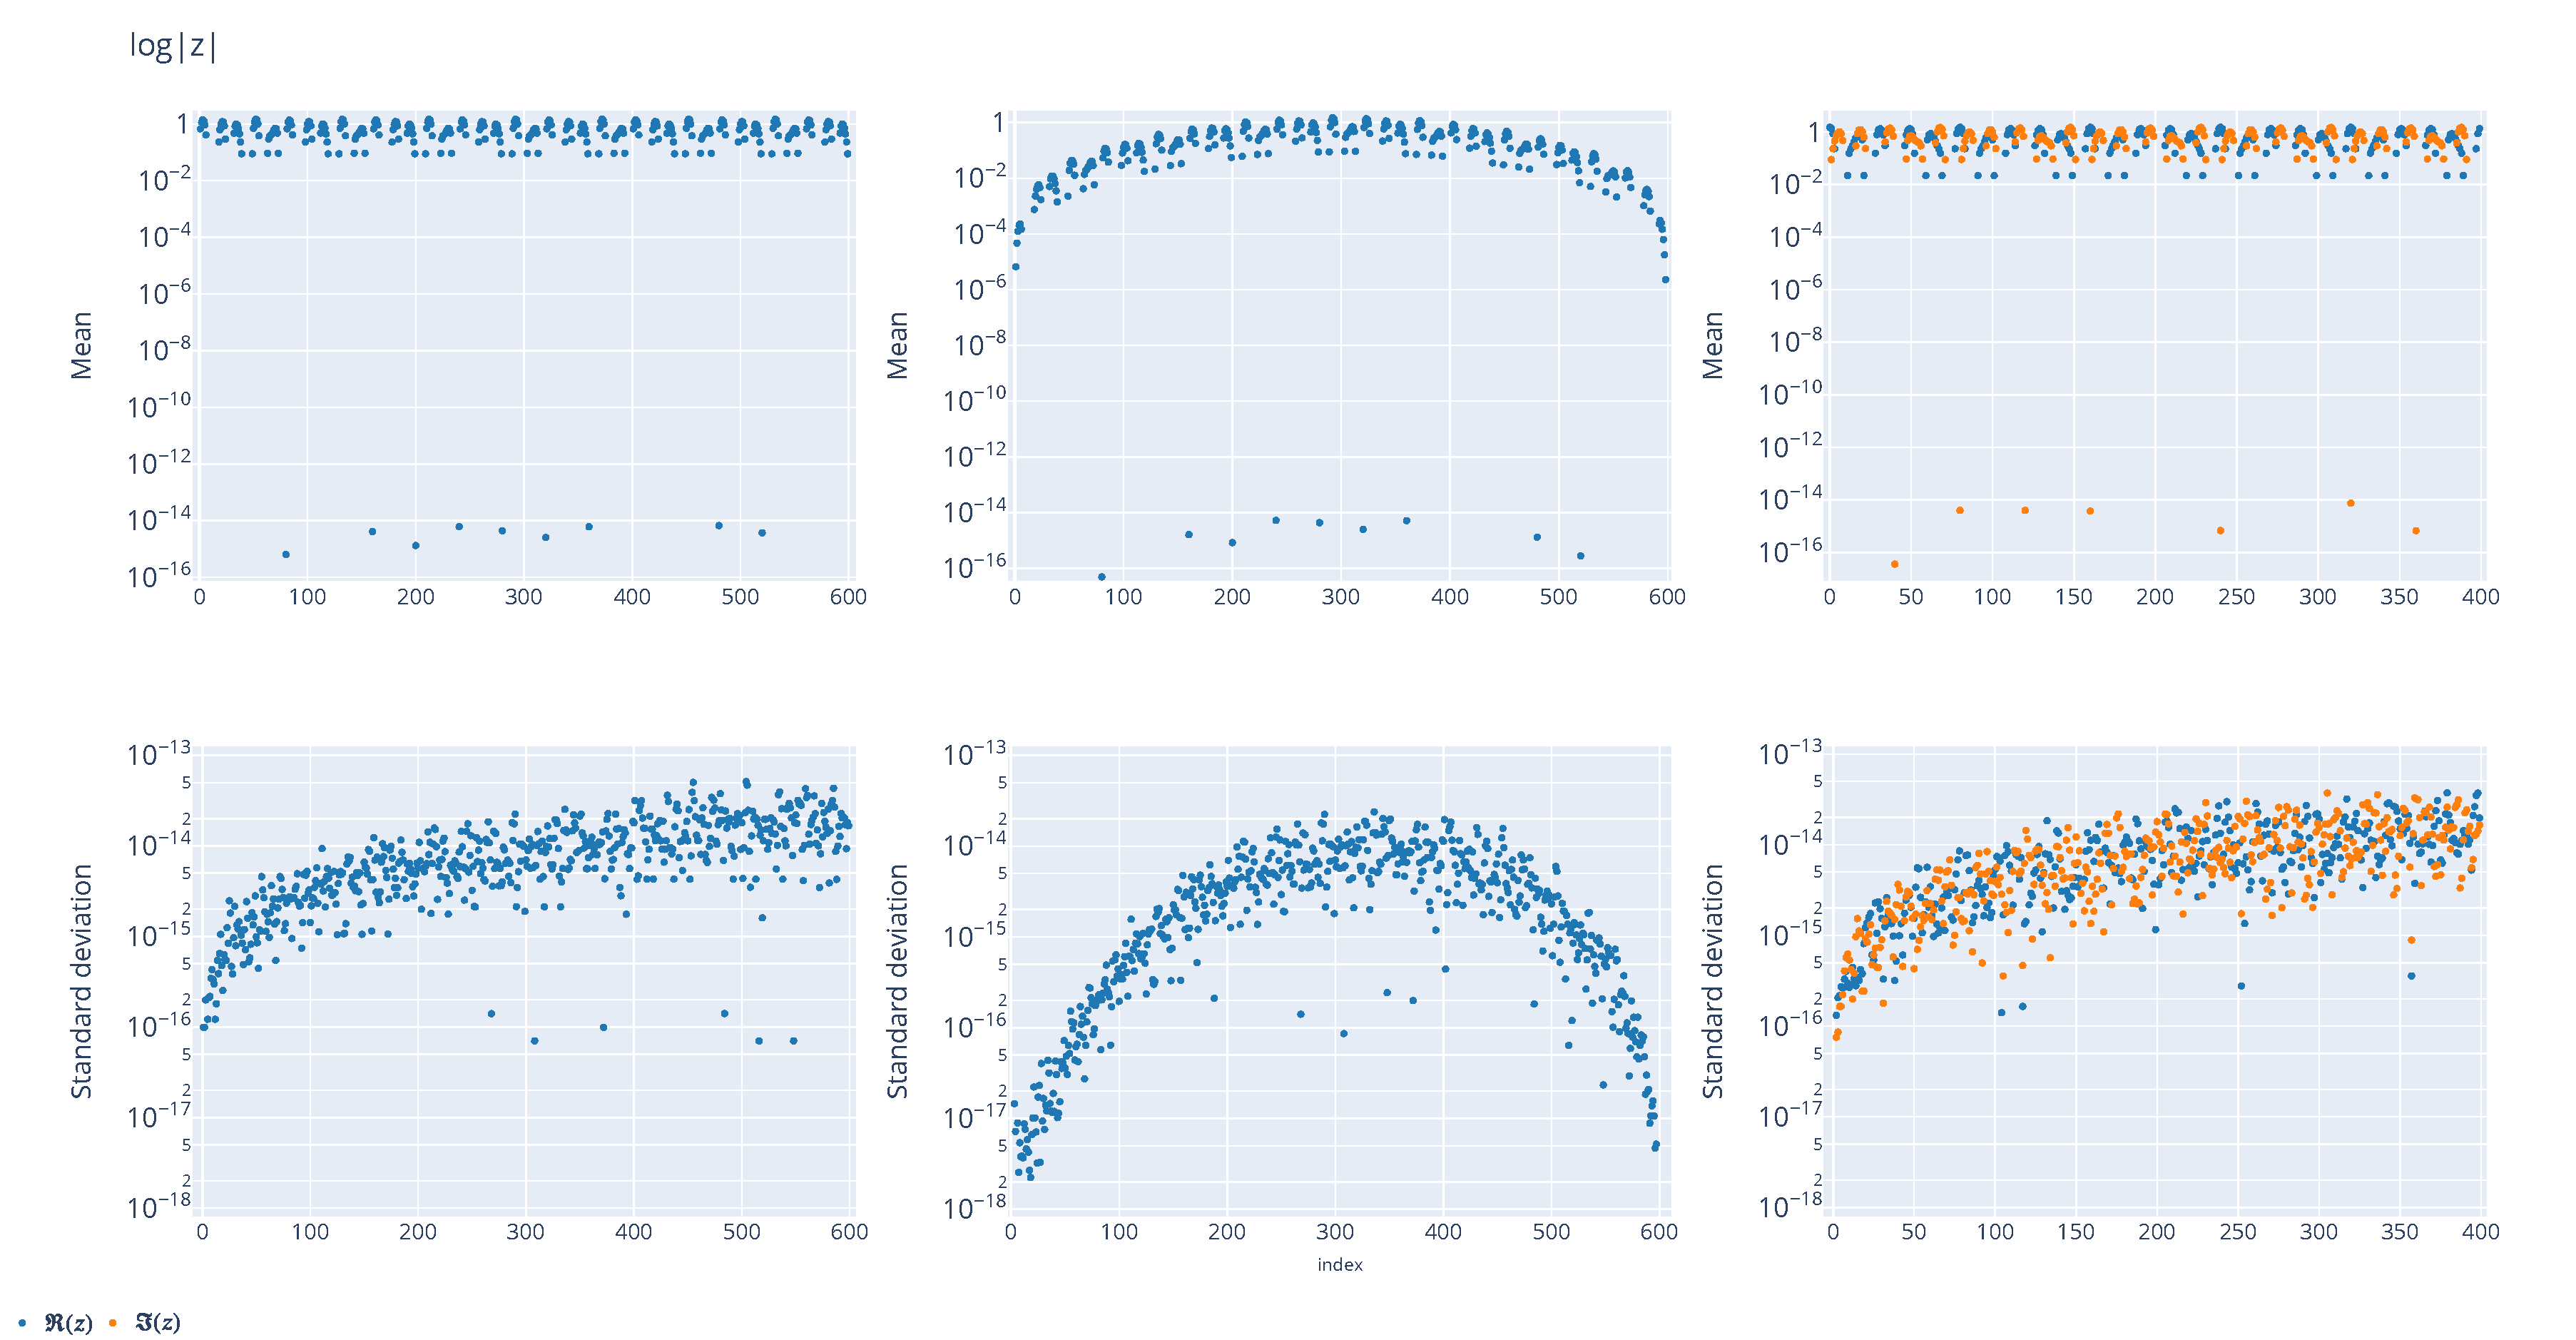
\includegraphics[width=\linewidth]{figure/FFT/fft_x.pdf}
    \caption{Absolute value of the mean and standard deviation values for 
    fft 1D inputs within RR mode (log scale).}
    \label{fig:fft1D_mean}
\end{figure}

\begin{figure}
    \centering
    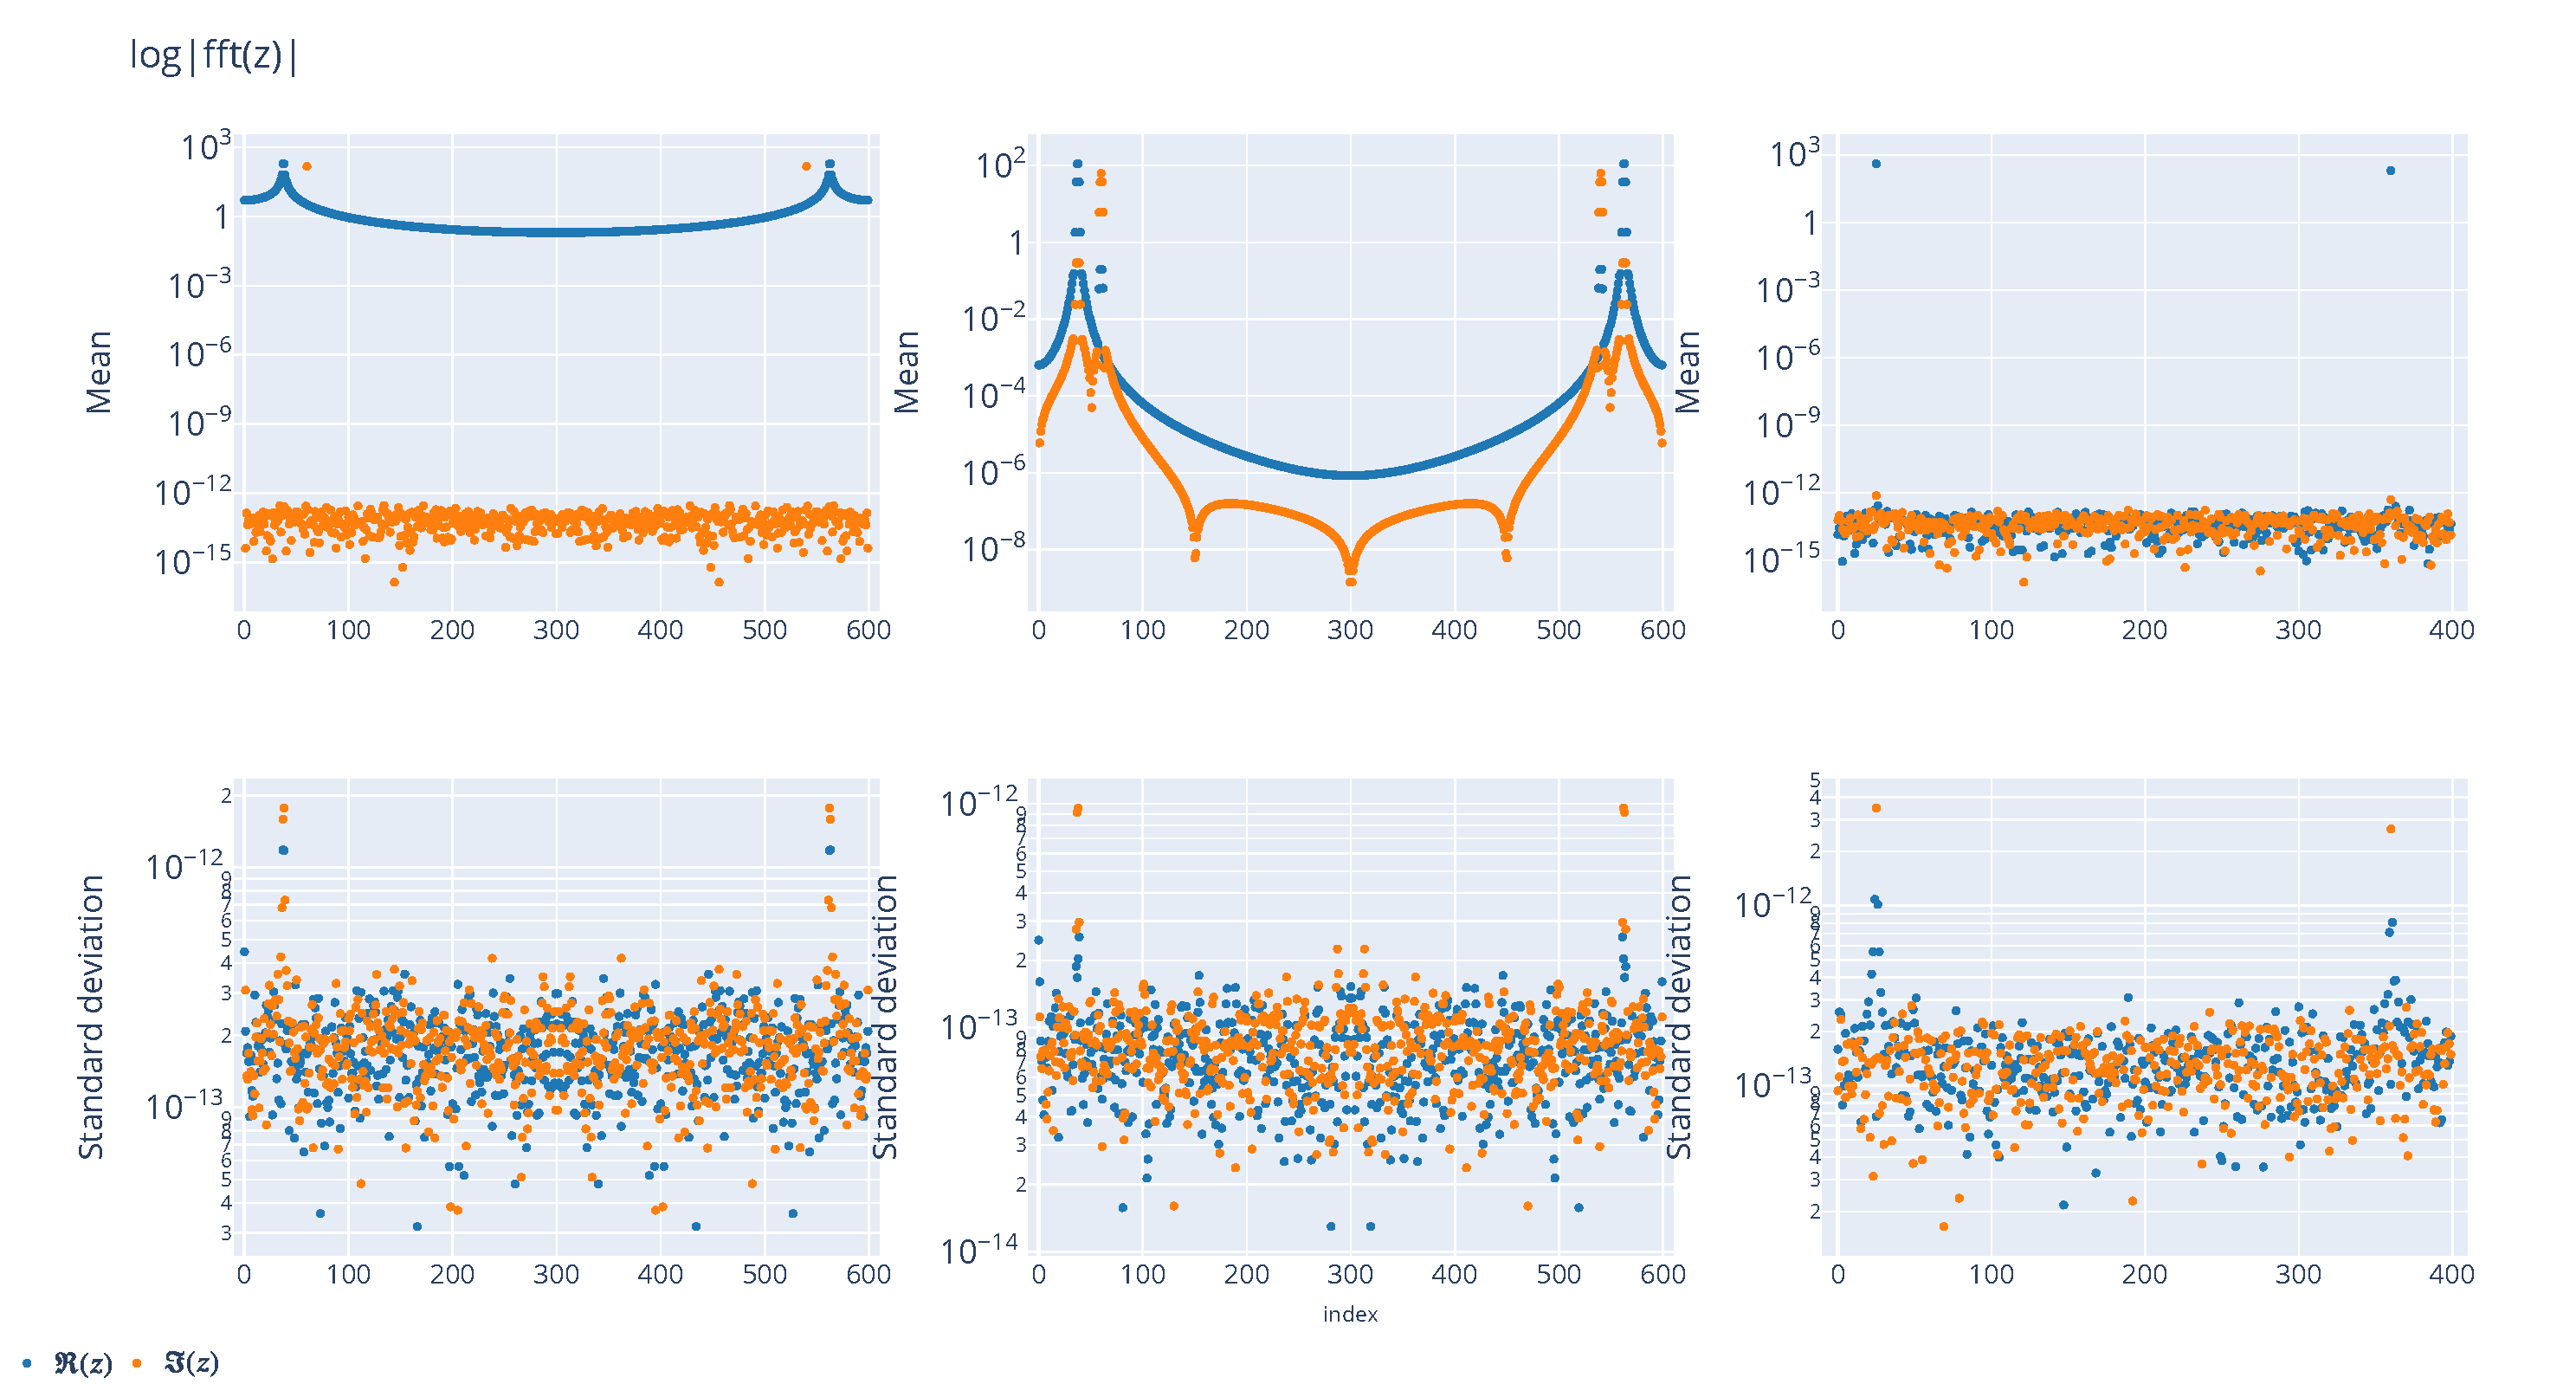
\includegraphics[width=\linewidth]{figure/FFT/fft_y.pdf}
    \caption{Absolute value of the mean and standard deviation values 
    for fft 1D outputs within RR mode (log scale).}
    \label{fig:fft1D_std}
\end{figure}

% \begin{figure}
% \begin{minipage}{.5\textwidth}
%     \centering
%     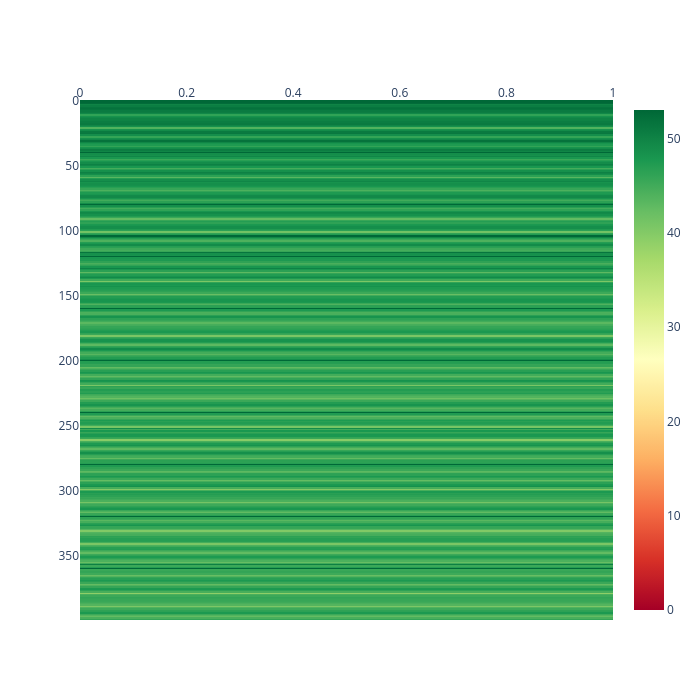
\includegraphics[width=\linewidth]{figure/FFT/fft_x_real_sig_36.png}
%     \caption{$\Re(x)$}
%     \label{fig:my_label}
% \end{minipage}
% \begin{minipage}{.5\textwidth}
%     \centering
%     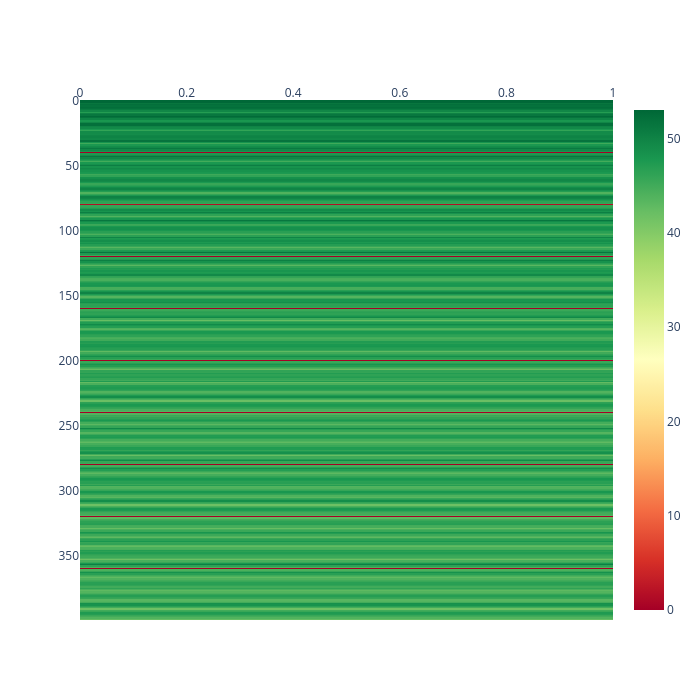
\includegraphics[width=\linewidth]{figure/FFT/fft_x_imag_sig_36.png}
%     \caption{$\Im(x)$}
%     \label{fig:my_label}
% \end{minipage}
% \begin{minipage}{.5\textwidth}
%     \centering
%     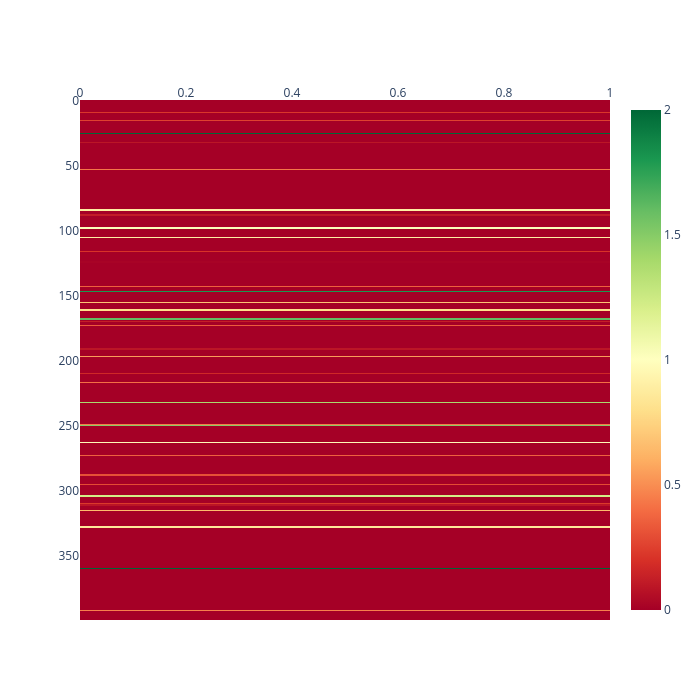
\includegraphics[width=\linewidth]{figure/FFT/fft_ret_real_sig_36.png}
%     \caption{$\Re$(fft$(x))$}
%     \label{fig:my_label}
% \end{minipage}
% \begin{minipage}{.5\textwidth}
%     \centering
%     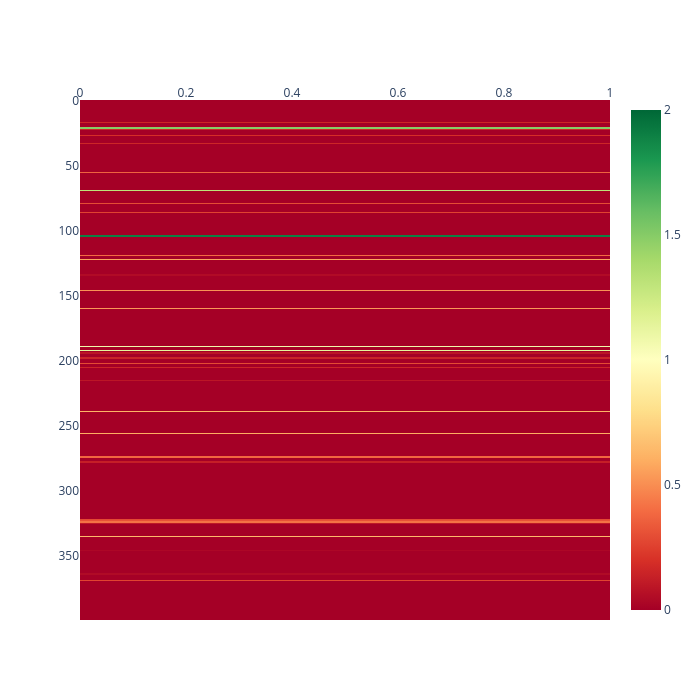
\includegraphics[width=\linewidth]{figure/FFT/fft_ret_imag_sig_36.png}
%     \caption{$\Im$(fft$(x))$}
%     \label{fig:my_label}
% \end{minipage}
% \end{figure}


\subsection{Interpolation}

This package has three tests: \texttt{interpolation\_1D}, \texttt{multivariate\_data}, \texttt{bspline}, \texttt{spline\_1D} and \texttt{spline\_2D}.

The \texttt{interpolation\_1D} test interpolates the function $\cos(\frac{-x^2}{9})$ with 11 points $x\in[0,10]$.
For the fives schemes tested (linear, cubic, nearest, previous, next), the solution found is precise, up to 51 bits out of the 53 available.

The \texttt{multivariate\_data} test interpolates the grid $f(x,y)=x(1-x)\cos(4\pi.x)  \sin(4\pi.y^2)^2$ with $(x,y) \in [0,1] \times [0,1]$ sampling with 1000 points for each coordinate using three schemes: nearest, linear and cubic. Our results show a precision of 51 bits in average for the three schemes. 

The \texttt{bspline} test compares two edge filters: \texttt{bisplev} that evaluates a bivariate B-spline and its derivative and \texttt{convolved2d} that convolves two 2-dimensional arrays. Figure~\ref{fig:bspline_rr}
shows the significant bits (figs.~\ref{fig:bspline_bisplev_sig},~\ref{fig:bspline_convol2d_sig}), 
mean (figs.~\ref{fig:bspline_bisplev_mean},~\ref{fig:bspline_convol2d_mean}), and standard deviation (figs.~\ref{fig:bspline_bisplev_std},~\ref{fig:bspline_convol2d_std}) maps for the two methods as well as the input image (fig.~\ref{fig:bspline_input}) with the middle for the \texttt{bisplev} results and bottom row for the \texttt{convol2d}. We can see no visual differences between both methods with 11 significant bits in average. Standard deviations maps on figures~\ref{fig:bspline_bisplev_std} and~\ref{fig:bspline_convol2d_std} show that regions with low spatial frequencies correspond to regions with low standard deviation, similar to the FFT results. As it is mentioned in the SciPy tutorial, the \texttt{bisplev} function is faster than the \texttt{convol2d} while our experiments show that they have the same numerical precision which reinforces the use of \texttt{bisplev} over \texttt{convol2d} in this example.

The \texttt{spline\_1D} test computes the 1D spline interpolation for the function $\sin(x)$ on points $x=\frac{2\pi k}{8}, k \in [0, 10]$. The spline interpolation uses two methods: \texttt{splrep} to build the spline representation and \texttt{splrev} to evaluate the spline at any point. It also computes the integral by using \texttt{splint} and the root finder \texttt{sproot}. Although the traces diverge, we can analyze the partial aggregation for the \texttt{splrep}, \texttt{splev} and \texttt{splint}. The three functions show results with an average precision of 51 bits with RR mode.
 
The \texttt{spline\_2D} test computes the 2D spline interpolation for the function $z=(x+y)e^{-6(x^2+y^2)}$, with $(x,y) \in [-1,1]\times[-1,1]$ sampling with 21 points for each coordinate. \texttt{bisplrep} builds the spline representation with the $21 \times 21$ points of $z$ over a 71 grid sampling points for $(x,y)$. The figure~\ref{fig:spline2d_rr} shows the results of the spline evaluation with \texttt{bisplev}. 


% \begin{figure}
% \begin{minipage}{.3\textwidth}
%     \centering
%     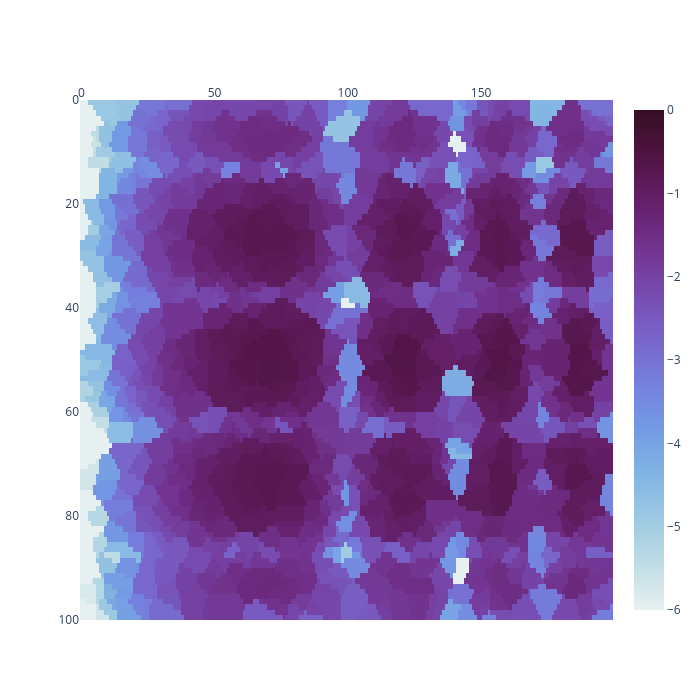
\includegraphics[width=\linewidth]{figure/multivariate_data/nearest_ret_mean_log.png}
% \end{minipage}
% \begin{minipage}{.3\textwidth}
%     \centering
%     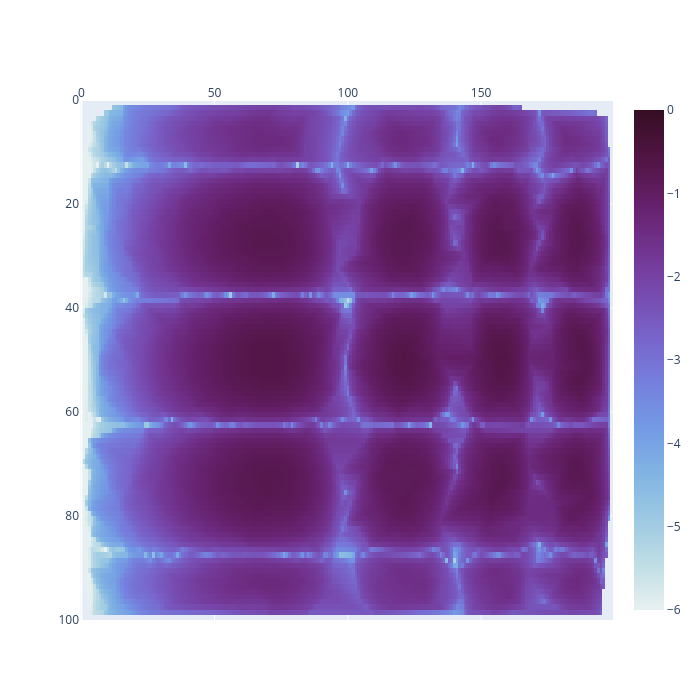
\includegraphics[width=\linewidth]{figure/multivariate_data/linear_ret_mean_log.png}
% \end{minipage}
% \begin{minipage}{.3\textwidth}
%     \centering
%     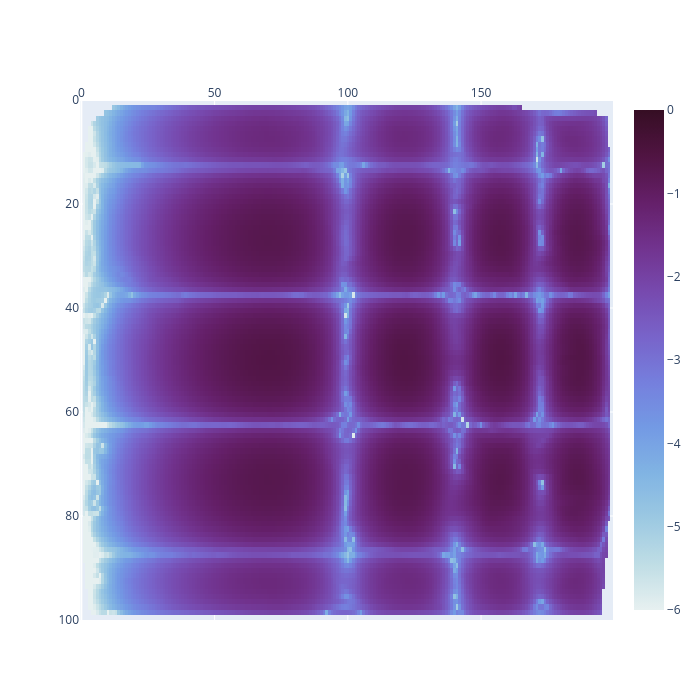
\includegraphics[width=\linewidth]{figure/multivariate_data/cubic_ret_mean_log.png}
% \end{minipage}

% \begin{minipage}{.3\textwidth}
%     \centering
%     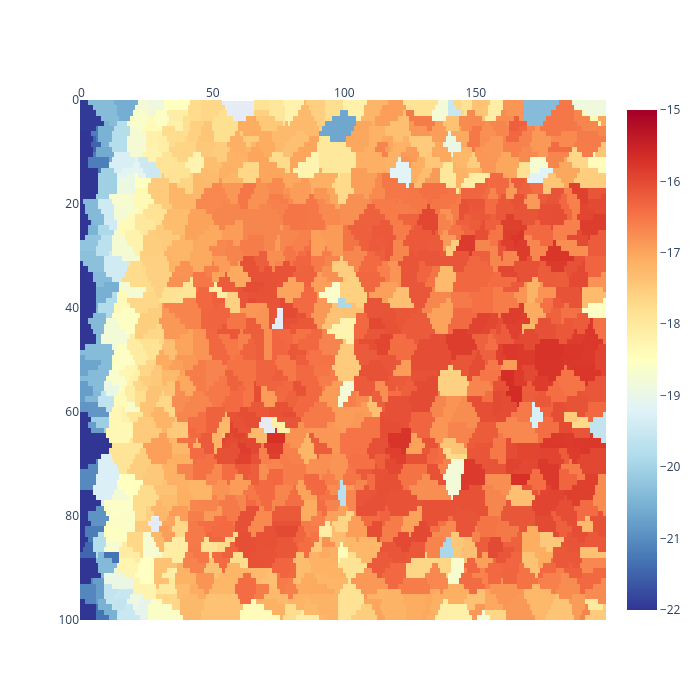
\includegraphics[width=\linewidth]{figure/multivariate_data/nearest_ret_std_log.png}
% \end{minipage}
% \begin{minipage}{.3\textwidth}
%     \centering
%     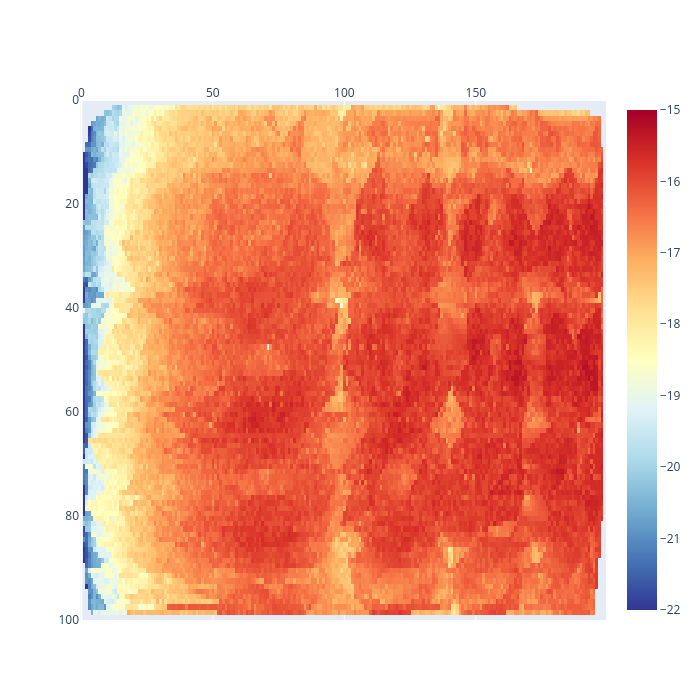
\includegraphics[width=\linewidth]{figure/multivariate_data/linear_ret_std_log.png}
% \end{minipage}
% \begin{minipage}{.3\textwidth}
%     \centering
%     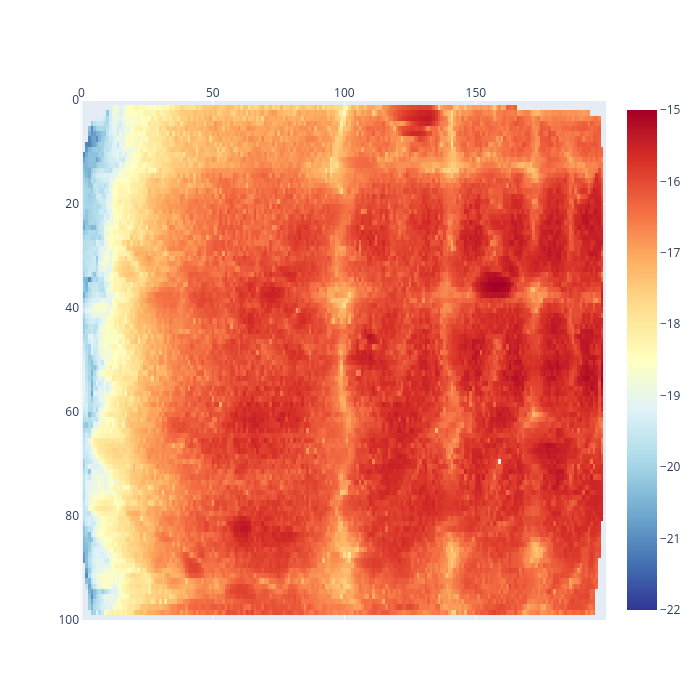
\includegraphics[width=\linewidth]{figure/multivariate_data/cubic_ret_std_log.png}
% \end{minipage}
%     \label{fig:multivariate_data_RR}
%     \caption{\texttt{multivariate\_data} results within RR mode. Each column represents an 
%     interpolation scheme, with from left to right, the nearest, linear and cubic method.
%     Top row shows the log of the absolute mean value value while bottom row shows the log of the
%     standard deviation. We can see that precision drops between local extremum when the 
%     mean value is close to 0.}
% \end{figure}

\begin{figure}
\centering
\begin{subfigure}{.3\linewidth}
    \includegraphics[width=\linewidth]{}
\end{subfigure}
\begin{subfigure}{.3\linewidth}
    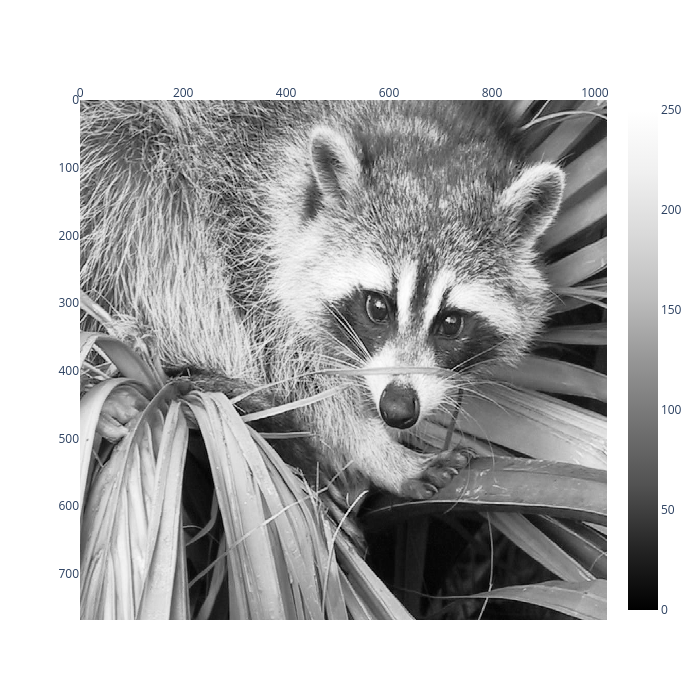
\includegraphics[width=\linewidth]{figure/bspline/original_image.png}
    \caption{}
    \label{fig:bspline_input}
\end{subfigure}
\begin{subfigure}{.3\linewidth}
    \includegraphics[width=\linewidth]{}
\end{subfigure}
\begin{subfigure}{0.3\linewidth}
    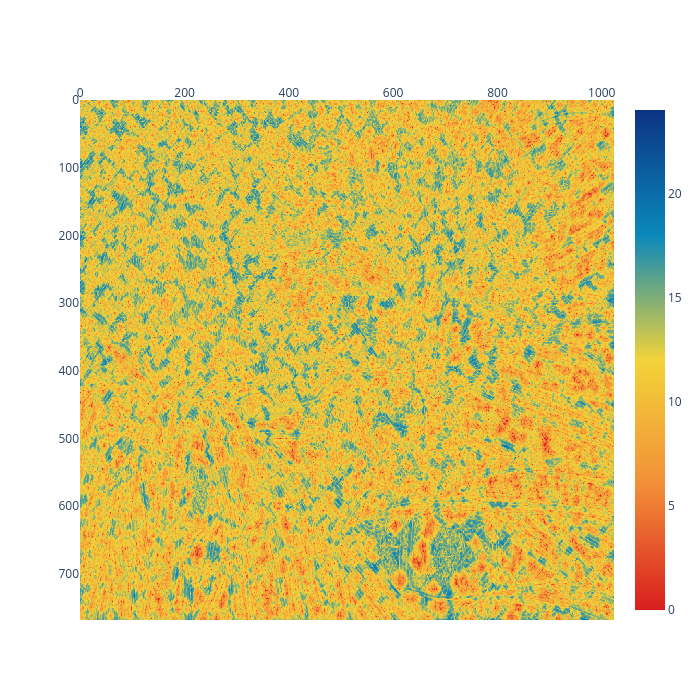
\includegraphics[width=\linewidth]{figure/bspline/bisplev_ret_sig_portland_r.png}
    \caption{}
    \label{fig:bspline_input}
    \label{fig:bspline_bisplev_sig}
\end{subfigure}
\begin{subfigure}{0.3\linewidth}
    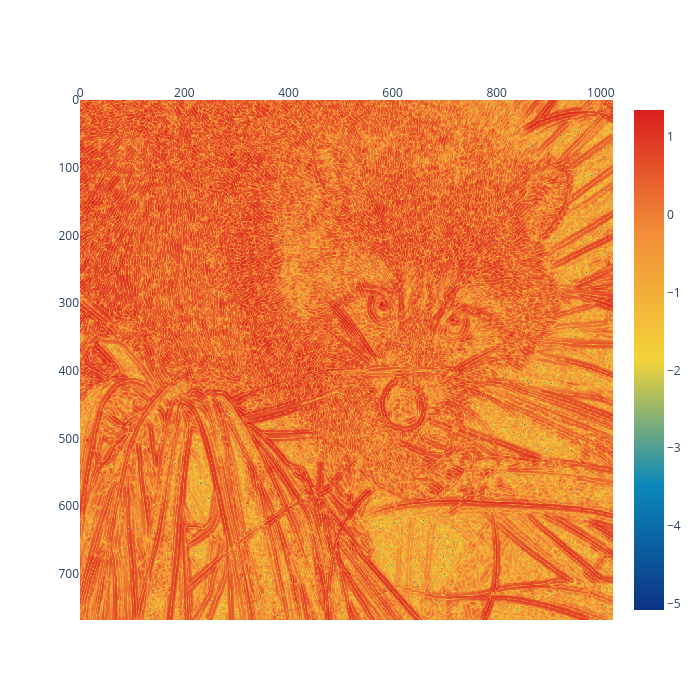
\includegraphics[width=\linewidth]{figure/bspline/bisplev_ret_mean_log_portland.png}
    \caption{}
    \label{fig:bspline_bisplev_mean}
\end{subfigure}
\begin{subfigure}{0.3\linewidth}
    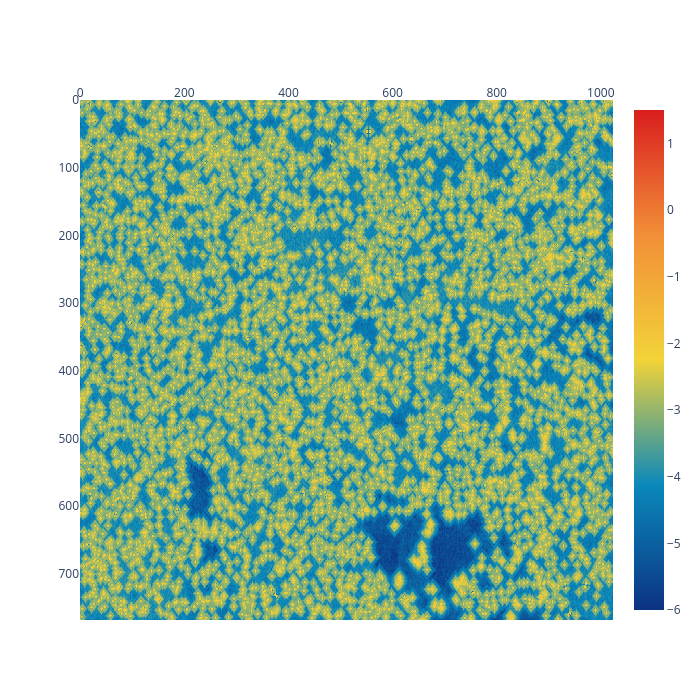
\includegraphics[width=\linewidth]{figure/bspline/bisplev_ret_std_log_portland.png}
    \caption{}
    \label{fig:bspline_bisplev_std}
\end{subfigure}
\begin{subfigure}{0.3\linewidth}
    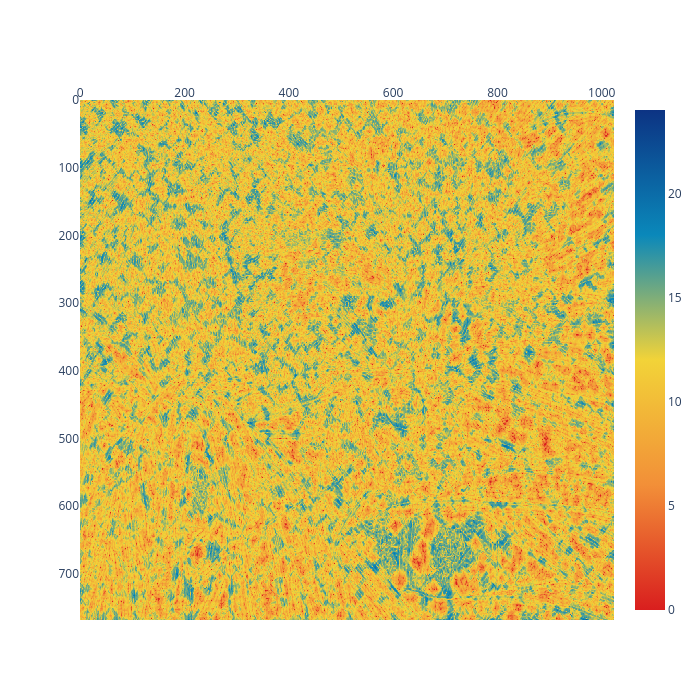
\includegraphics[width=\linewidth]{figure/bspline/convol2d_ret_sig_portland_r.png}
    \caption{}
    \label{fig:bspline_convol2d_sig}
\end{subfigure}
\begin{subfigure}{0.3\linewidth}
    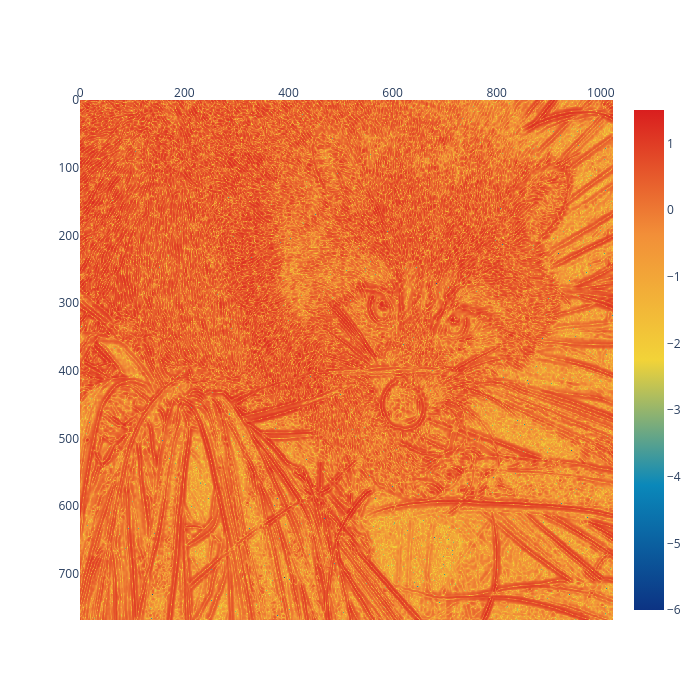
\includegraphics[width=\linewidth]{figure/bspline/convol2d_ret_mean_log_portland.png}
    \caption{}
    \label{fig:bspline_convol2d_mean}
\end{subfigure}
\begin{subfigure}{0.3\linewidth}
    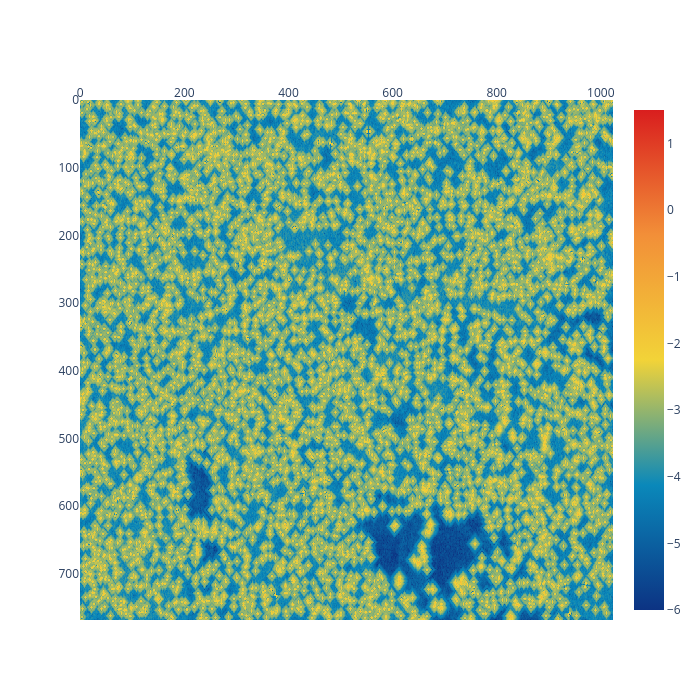
\includegraphics[width=\linewidth]{figure/bspline/convol2d_ret_std_log_portland.png}
    \caption{}
    \label{fig:bspline_convol2d_std}
\end{subfigure}
    \label{fig:bspline_rr}
    \caption{\texttt{bspline} results within RR mode. Left column shows the \texttt{bisplev} function
    while the right column shows the \texttt{convolve2d} function. }
\end{figure}

\begin{figure}
\begin{subfigure}{.3\textwidth}
    \centering
    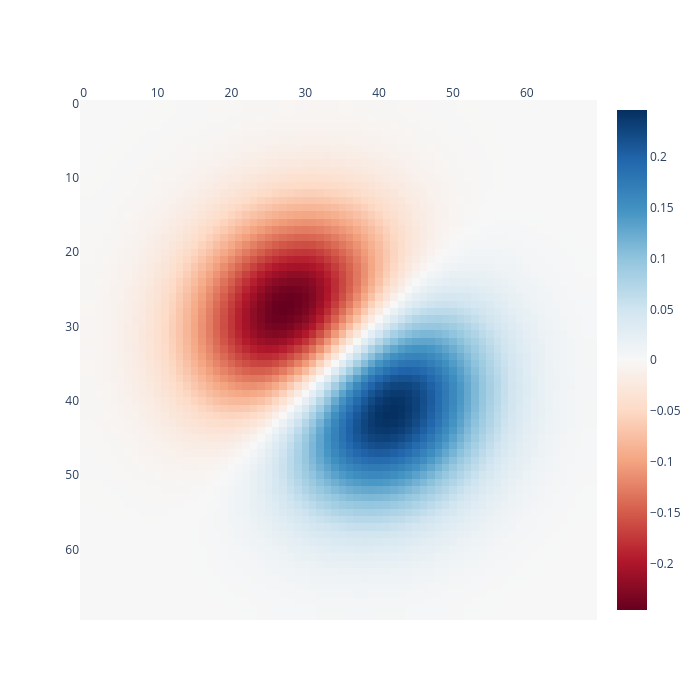
\includegraphics[width=\linewidth]{figure/spline_2d/bisplev_inputs_mean.png}
    \caption{\texttt{bisplev} IEEE result}
    \label{fig:bisplev_ieee}
\end{subfigure}
\begin{subfigure}{.3\textwidth}
    \centering
    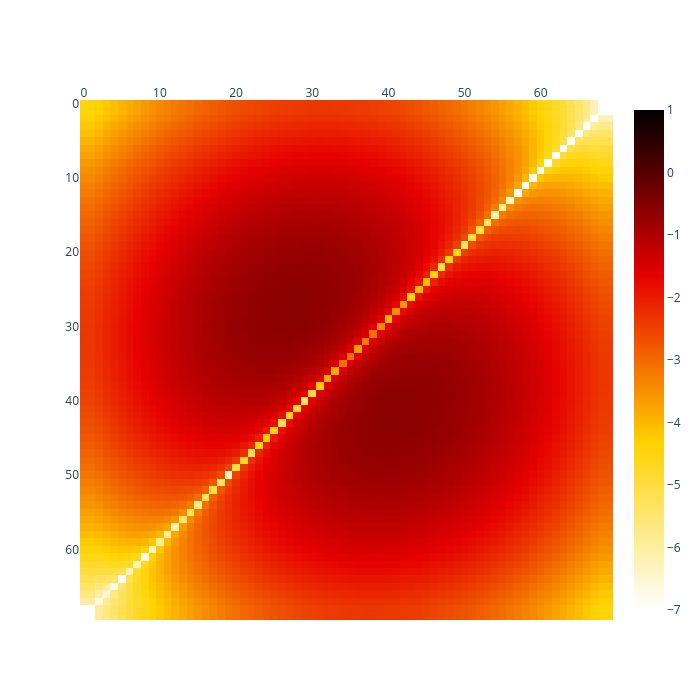
\includegraphics[width=\linewidth]{figure/spline_2d/bisplev_inputs_mean_log.png}
    \caption{Absolute mean value (log)}
    \label{fig:bisplev_mean_log}
\end{subfigure}
\begin{subfigure}{.3\textwidth}
    \centering
    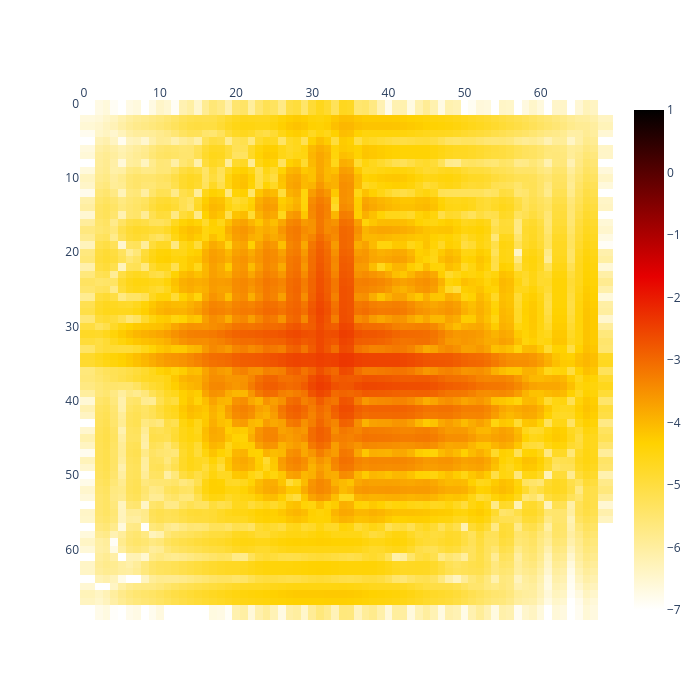
\includegraphics[width=\linewidth]{figure/spline_2d/bisplev_inputs_std_log.png}
    \caption{Standard deviation (log)}
    \label{fig:bisplev_std_log}
\end{subfigure}
    \caption{2D Spline interpolation results. Figure~\ref{fig:bisplev_ieee} shows the IEEE result
    of the 2D-spline interpolation. Figures~\ref{fig:bisplev_mean_log} and~\ref{fig:bisplev_std_log}
    show respectively in the logarithmic scale the absolute mean value and the standard deviation 
    of the 5 samples run within RR mode.}
    \label{fig:spline2d_rr}
\end{figure}


\subsubsection{Optimization}

This package has ten tests: five for unconstrained minimization of multivariate scalar functions using different algorithms: \texttt{Nelder-Mead}~\cite{singer2009nelder} that iteratively transforms a simplex until its vertices are getting closer to local minima of the function. Fours Quasi-Newton-Raphson methods whose main goal is to determine $x$ that minimizes the function $f$ by using Newton's method step: $x_{k+1} = x_{k} - B^{-1}(x_k)\nabla f(x_k)$, where $\nabla$ and $B$ are the gradient and the approximation of the Hessian matrix of $f$. The \texttt{Broyden-Fletcher-Goldfarb-Shanno}~\cite{BFGS} (BFGS) and \texttt{Newton-Conjugate-Gradient}~\cite{nocedal2006numerical} (NCG) are line search methods that respectively approximates $H$ by adding two symmetric rank-one matrices and by using the Conjugate-Gradient method. The \texttt{Trust-Region Truncated Generalized Lanczos / Conjugate Gradient}~\cite{gould1999solving}, \texttt{Trust-Region Newton-Conjugate-Gradient} and \texttt{Trust-Region Nearly Exact}~\cite{nocedal2006numerical} are trust-region methods that approximates $H$ by solving the trust-region subproblem restricted to a truncated Krylov subspace and by solving nonlinear equations for each quadratic subproblem. Two tests for constrained minimization of multivariate scalar functions: \texttt{Sequential Least SQuares Programming} (SLSQP) and \texttt{Least-squares minimization}.
And three for root finding with one for small problems \texttt{root\_finding} and two for large problems using a Krylov approximation for the inverse Jacobian with and without the help of a preconditioner: \texttt{root\_finding\_large\_preconditionned} and \texttt{root\_finding\_large}.

The unconstrained minimization of multivariate scalar minimizes the Rosenbrock function of $N$ variables:
\[f(x) = \sum_{i=1}^{N-1} 100(x_{i+1}-x^2_i)^2 + (1-x_i)^2\]
The minimum value of this function is 0, which is achieved when $x_i=1$.
Figure~\ref{fig:unconstrained_optimization} shows the number of significant bits of the solution for the different methods used. We can see that all methods have a good precision comprising between 43 and 53 bits significant. The Nelder-Mead method is the worst with $\simeq$ 43 bits on average, while the Trust-Region-Newton-CG has the best precision with $\simeq$ 53 bits significant, which is significant the maximum achievable within double precision. The remaining methods share a similar precision with less than 1 bit between them.

The constrained minimization of multivariate scalar tests minimize the Rosenbrock function for SLSQP subject to
\begin{eqnarray*}
    x_0 + 2x_1 \leq 1 \\
    x_0^2 + x_1 \leq 1 \\
    x_0^2 - x_1 \leq 1 \\
    2x_0 + x_1 = 1 \\
    0 \leq x_0 \leq 1 \\
    -0.5 \leq x_1 \leq 2 
\end{eqnarray*}
with the unique solution $[x_0, x_1] = [0.4149, 0.1701]$.
Results within RR show a precision of 47 and 44 bits for the first and the second solution.
The \texttt{least-square minimization} test solves a fitting problem from an enzymatic reaction~\cite{kowalik1968analysis} with 11 residuals defined as:
\begin{eqnarray*}
f_i(x) &=& \frac{x_0(u_i^2 + u_ix_1)}{u_i^2 + u_ix_2+x_3}-y_i,\; i=0,...,10 \\
&0& \leq x_j \leq 100,\; j=0,..,3
\end{eqnarray*}
where where $y_i$ are measurement values, $u_i$ are values of the independent variable, and
$x_i$ the unknown.
Results within RR show a precision of [51,46,47,48] bits for the solution.

Finally, the \texttt{root\_*} tests use three algorithms to 
find root of non-linear equations. \texttt{root\_finding}
uses the hybrid method of Powell to solve a single-variable transcendental equation and 
the Levenberg-Marquardt for a set of non-linear equations. 
\texttt{root\_finding\_large} and \texttt{root\_finding\_large\_preconditioned} tests use 
Krylov method to solve an integrodifferential equation on a square
 $(x,y) \in [0,1] \times [0,1]$, $P(x,1)=1$, and $P=0$ elsewhere on the boundary.
The function $P$ is discretized with a Cartesian grid $P_{n,n}=P(nh,nh)$, with $n=75$ and its derivatives are approximated by $\partial_x^2P(x,y) \simeq (P(x+h,y) - 2P(x,y) + P(x-h,y))/h^2$.

% the two following equations: $x + 2\cos(x) = 0$ and 
% the set $x_0\cos(x_1)=4$; $x_0x_1-x_1 = 5$ while the 
% \texttt{root\_finding\_large} and \texttt{root\_finding\_large\_preconditioned} tests 
% solve the equation:
% \[
%     (\partial_x^2 + \partial_y^2)P + 5 \left(\int_0^1 \int_0^1 cosh(P)\, dx dy \right)^2 = 0
% \]


All tests diverge even within RR mode, which is not surprising since root-finding methods can easily take a few extra steps to find the root depending on the starting point. Nevertheless, for the \texttt{root\_finding\_large} test, 3 traces among the 5 samples can be merged for both RR and MCA modes.
Figure~\ref{fig:root_finding_large} shows the mean and standard deviation of the result for these 3 samples. We can see that both RR and Full MCA found a similar solution, with a less precise one for Full MCA, although the spread between RR and MCA is small with a maximal standard deviation of $8.10^{-9}$ for MCA against $3.10^{-9}$ for RR mode. Finally, it is interesting to note the impact of the preconditioning on the result numerical quality, with a precision doubling between \texttt{root\_finding\_large} and \texttt{root\_finding\_large\_preconditioned} as table~\ref{tab:pytracer_test_precision_summary} shows.

\begin{figure}
    \centering
    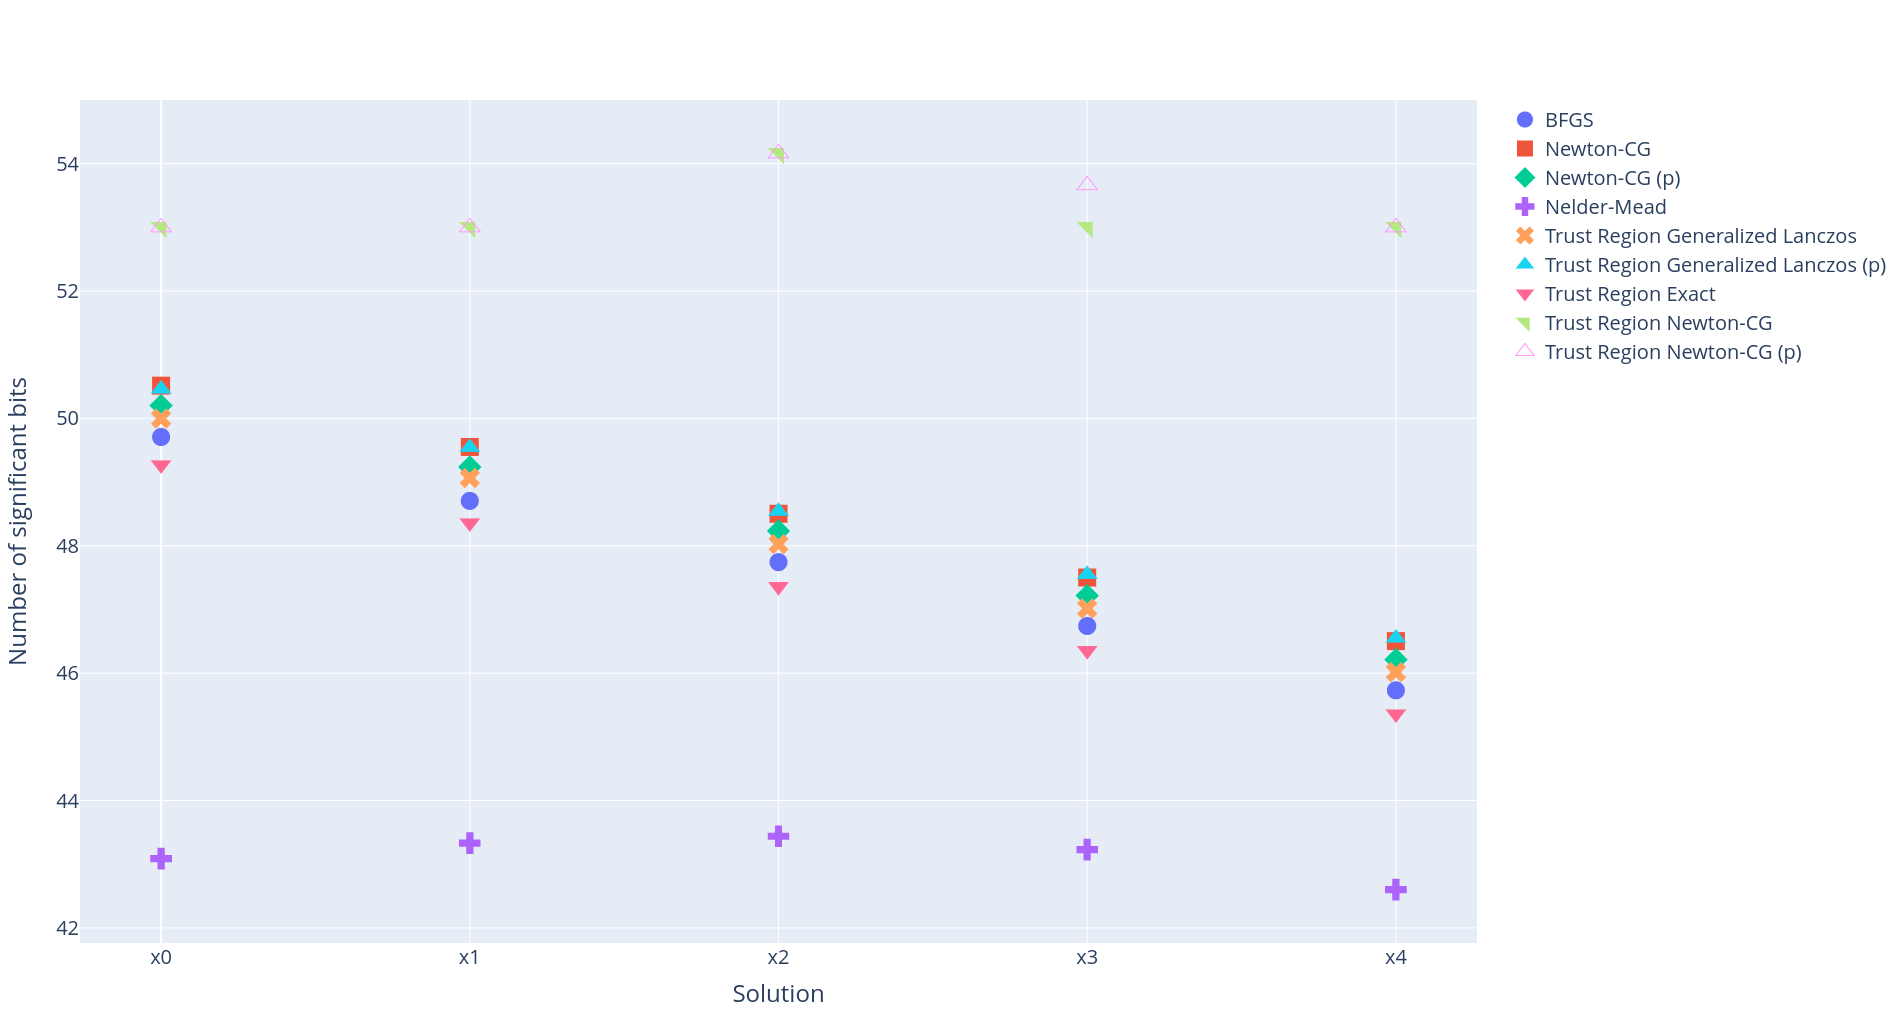
\includegraphics[width=\linewidth]{figure/unconstrained_optimization_comparison.png}
    \caption{Comparison of results precision for different optimization solvers within RR mode.}
    \label{fig:unconstrained_optimization}
\end{figure}

\begin{figure}
    \centering
    \begin{subfigure}{0.45\linewidth}
    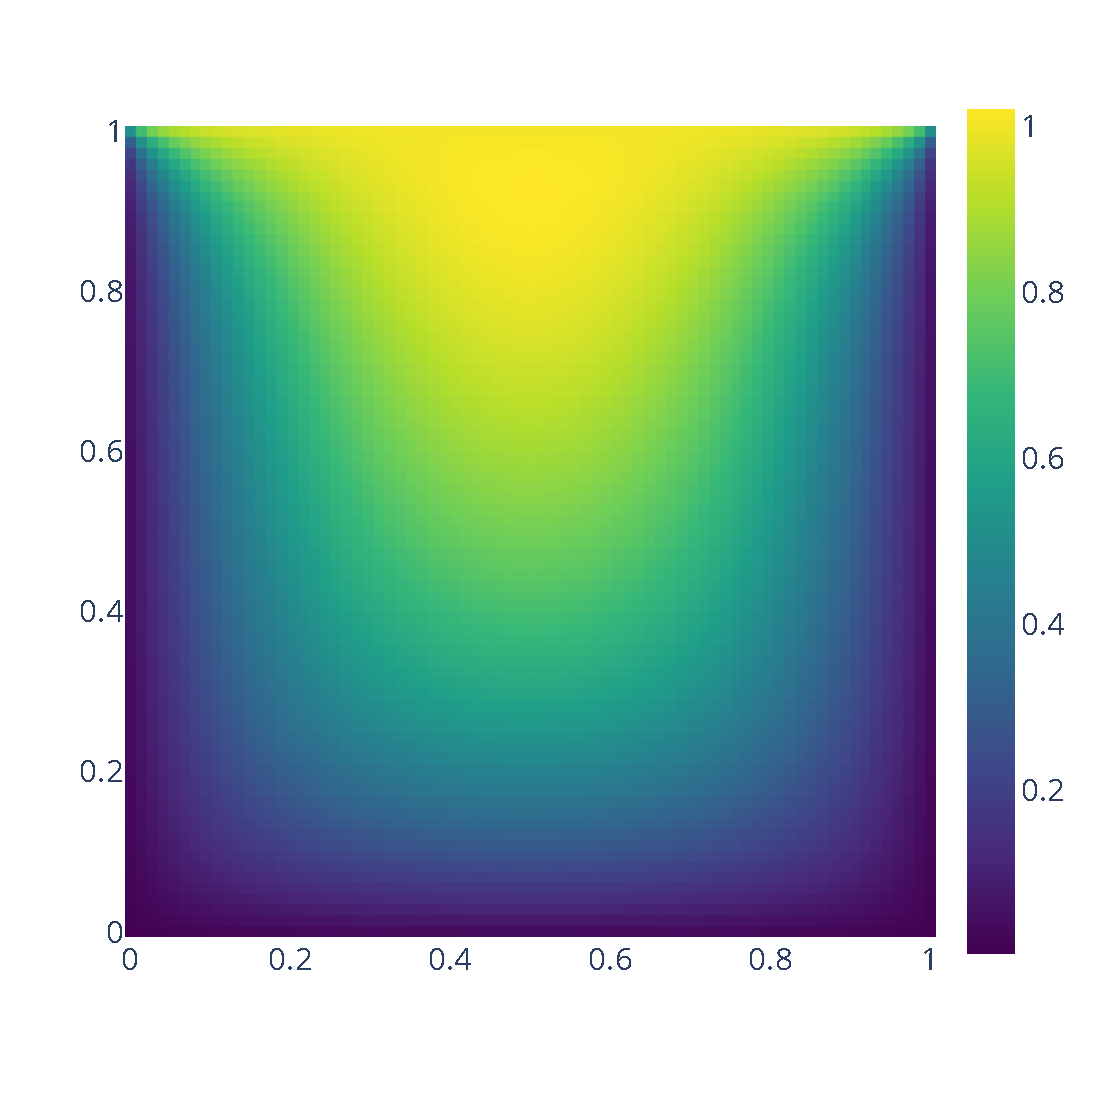
\includegraphics[width=\linewidth]{figure/root_finding/solution_mean_RR.pdf}
    \caption{}
    \label{fig:my_label}
    \end{subfigure}
    \begin{subfigure}{0.45\linewidth}
    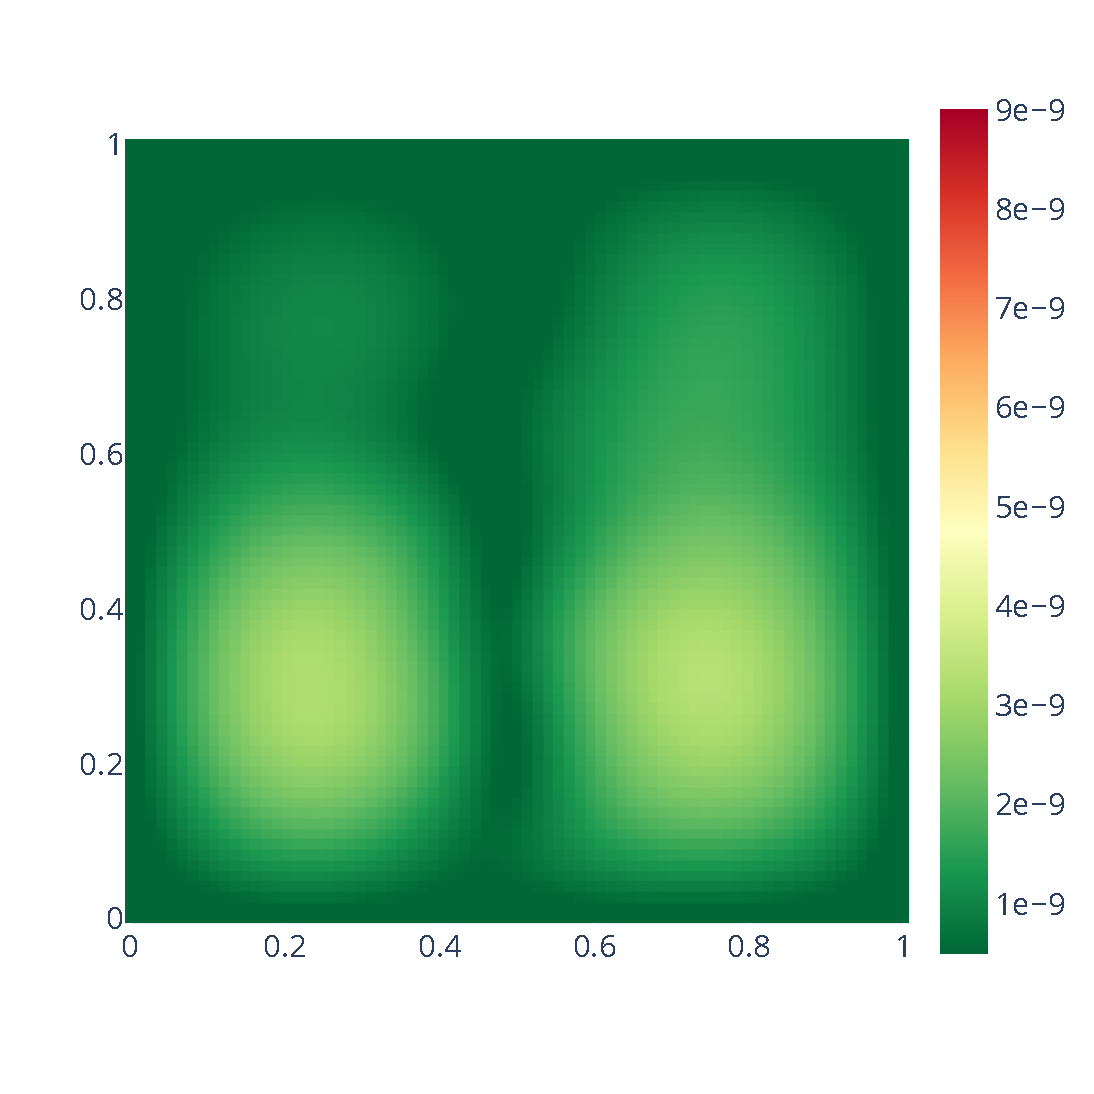
\includegraphics[width=\linewidth]{figure/root_finding/solution_std_RR.pdf}
    \caption{}
    \label{fig:my_label}
    \end{subfigure}
    
    \begin{subfigure}{0.45\linewidth}
    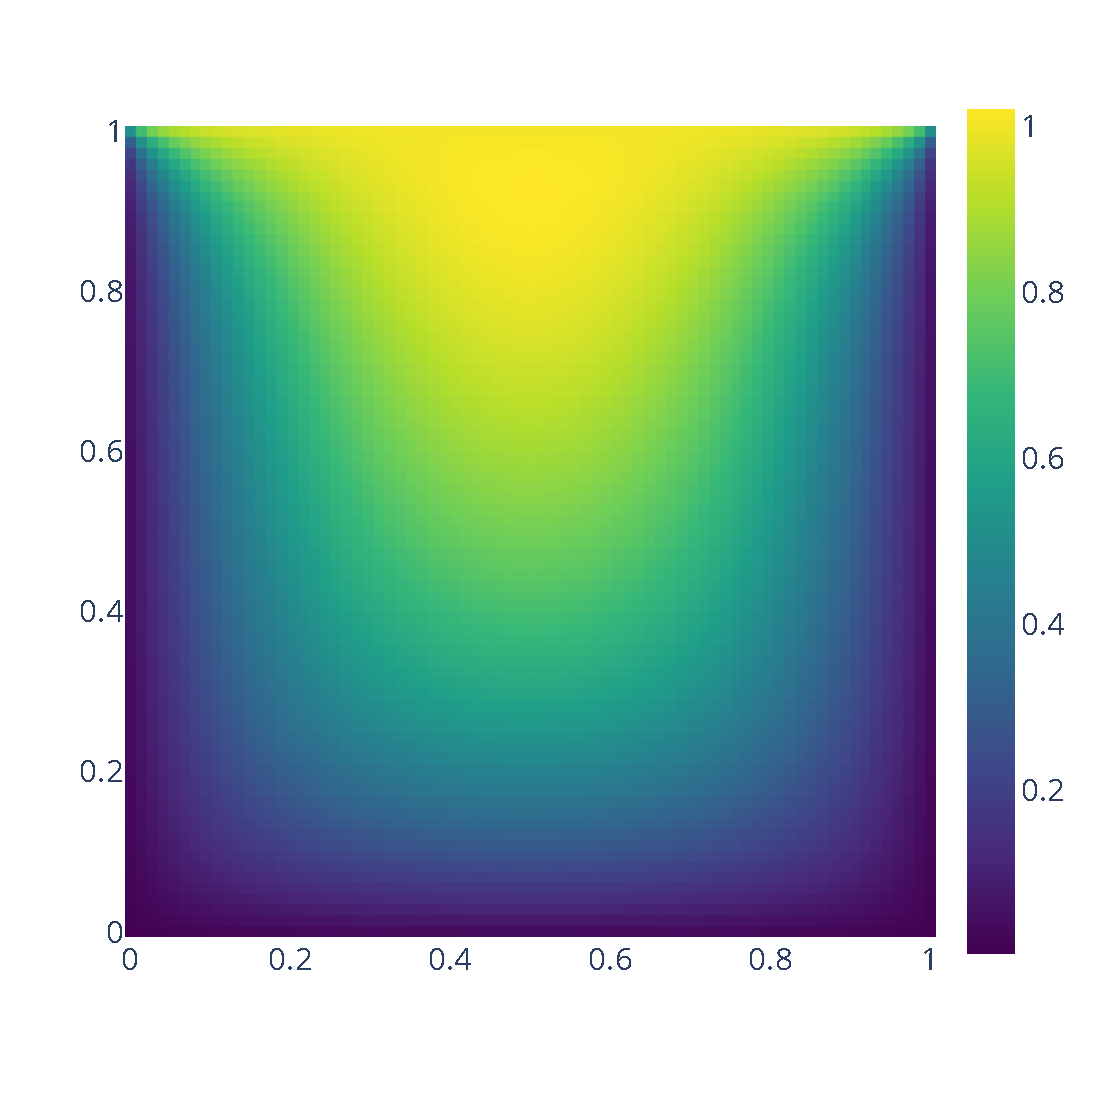
\includegraphics[width=\linewidth]{figure/root_finding/solution_mean_MCA.pdf}
    \caption{}
    \label{fig:my_label}
    \end{subfigure}
    \begin{subfigure}{0.45\linewidth}
    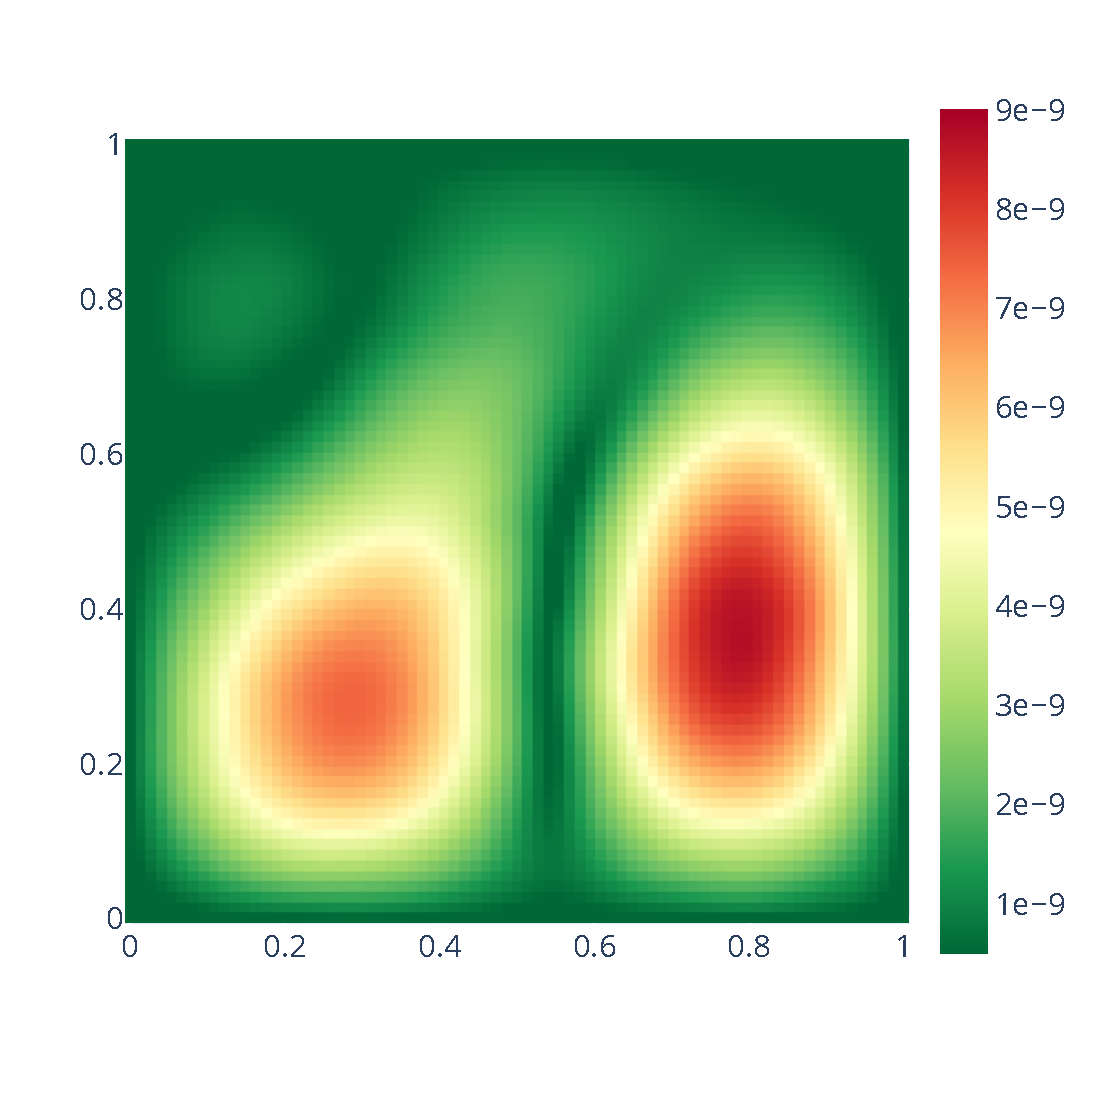
\includegraphics[width=\linewidth]{figure/root_finding/solution_std_MCA.pdf}    \caption{}
    \label{fig:my_label}
    \end{subfigure}
    \caption{Solution of \texttt{root\_finding\_large} test within RR (top row) and MCA (bottom row) with the mean value on the left and the standard deviation on the right. We can see that MCA has a less precision solution with a maximal standard deviation at $8.10^{-9}$ against $3.10^{-9}$ for RR mode. Moreover, we can see that a high standard deviation is localized around two extrema for both RR and Full MCA modes. Finally, the standard deviation stills lower than
    the stopping criterion threshold fixed at $6.10^{-6}$.}
    \label{fig:root_finding_large}
\end{figure}

% \begin{itemize}
% \item broyden: RR 47 bits solution / MCA divergence 
% \item global\_optimization: RR divergence / MCA issues
% \item sqlsp: RR 46 bits solution / MCA 46 bits solution
% \item least\_square\_minimization : RR 48 bits solution / MCA index issue
% \item nelder\_mean\_simplex : RR 43 bits solution / MCA stable
% \item newton\_conjugate\_gradient: RR 48 bits solution / MCA divergence
% \item root\_finding\_large\_preconditionned : RR divergence / MCA divergence 3/5 converged
% \item root\_finding\_large : RR divergence / MCA divergence (fgmres very low!) 3/5 converged
% \item trust\_region\_exact : RR 47 bit solution / RR 45 bit solution
% \item trust\_region\_truncated\_generalized\_lanczos : RR 48 bits solution / MCA 46 bits solution
% \end{itemize}

% \begin{figure}
%     \centering
%     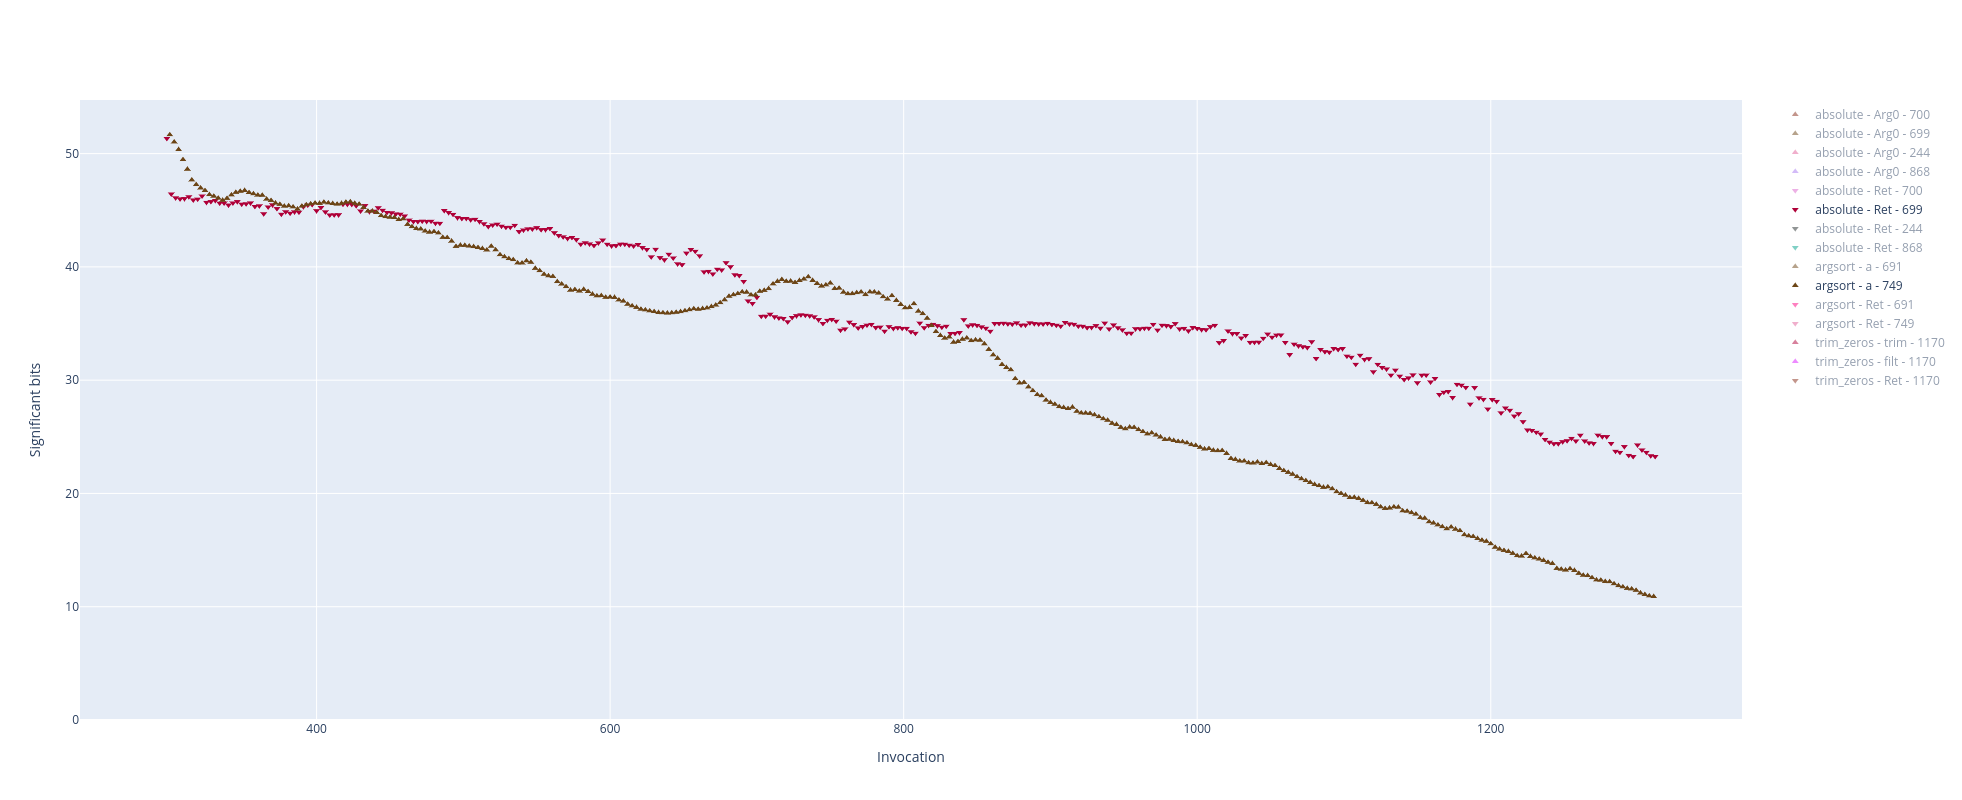
\includegraphics[width=\linewidth]{figure/nelder_mead/timeline_sig.png}
%     \caption{Nelder-Mead: average of number of significant bits over time. 
%     Solver ends when accuracy is reaching the tolerance.
%     }
%     \label{fig:my_label}
% \end{figure}

\subsection{Scikit learn}
\label{sec:sklearn_tests}

We tested Pytracer on the Scikit-learn~\cite{pedregosa2011scikit} library, a 
Python library implementing a wide range of state-of-the-art machine learning algorithms.
Scikit-learn offers a well supplied and documented list of examples that facilitates its using with Pytracer.
Among the several available examples, we choose the following representative set:
\href{https://scikit-learn.org/stable/auto_examples/ensemble/plot_adaboost_regression.html#sphx-glr-auto-examples-ensemble-plot-adaboost-regression-py}{Decision Tree Regression with AdaBoost},
\href{https://scikit-learn.org/stable/auto_examples/linear_model/plot_bayesian_ridge.html#sphx-glr-auto-examples-linear-model-plot-bayesian-ridge-py}{Bayesian Ridge Regression}, 
\href{https://scikit-learn.org/stable/auto_examples/linear_model/plot_sgd_comparison.html#sphx-glr-auto-examples-linear-model-plot-sgd-comparison-py}{Comparing various online solvers}, 
\href{https://scikit-learn.org/stable/auto_examples/cluster/plot_cluster_iris.html#sphx-glr-auto-examples-cluster-plot-cluster-iris-py}{K-means Clustering},
\href{https://scikit-learn.org/stable/auto_examples/covariance/plot_mahalanobis_distances.html#sphx-glr-auto-examples-covariance-plot-mahalanobis-distances-py}{Covariance Estimation},
\href{https://scikit-learn.org/stable/auto_examples/tree/plot_tree_regression.html#sphx-glr-auto-examples-tree-plot-tree-regression-py}{Decision Tree Regression},
\href{https://scikit-learn.org/stable/auto_examples/linear_model/plot_sgd_comparison.html#sphx-glr-auto-examples-linear-model-plot-sgd-comparison-py}{Recognizing hand-written digits},
\href{https://scikit-learn.org/stable/auto_examples/decomposition/plot_faces_decomposition.html#sphx-glr-auto-examples-decomposition-plot-faces-decomposition-py}{Faces dataset decomposition},
\href{https://scikit-learn.org/stable/auto_examples/linear_model/plot_logistic_l1_l2_sparsity.html#sphx-glr-auto-examples-linear-model-plot-logistic-l1-l2-sparsity-py}{L1 Penalty and Sparsity in Logistic Regression},
\href{https://scikit-learn.org/stable/auto_examples/linear_model/plot_lasso_and_elasticnet.html#sphx-glr-auto-examples-linear-model-plot-lasso-and-elasticnet-py}{Lasso and Elastic Net for Sparse Signals},
\href{https://scikit-learn.org/stable/auto_examples/linear_model/plot_sgd_separating_hyperplane.html#sphx-glr-auto-examples-linear-model-plot-sgd-separating-hyperplane-py}{SGD: Maximum margin separating hyperplane},
\href{https://scikit-learn.org/stable/auto_examples/linear_model/plot_sparse_logistic_regression_mnist.html#sphx-glr-auto-examples-linear-model-plot-sparse-logistic-regression-mnist-py}{MNIST classification using multinomial logistic + L1},
\href{https://scikit-learn.org/stable/auto_examples/linear_model/plot_sgd_iris.html#sphx-glr-auto-examples-linear-model-plot-sgd-iris-py}{Plot multi-class SGD on the iris dataset},
\href{https://scikit-learn.org/stable/auto_examples/linear_model/plot_multi_task_lasso_support.html#sphx-glr-auto-examples-linear-model-plot-multi-task-lasso-support-py}{Joint feature selection with multi-task Lasso},
\href{https://scikit-learn.org/stable/auto_examples/linear_model/plot_omp.html#sphx-glr-auto-examples-linear-model-plot-omp-py}{Orthogonal Matching Pursuit},
\href{https://scikit-learn.org/stable/auto_examples/decomposition/plot_pca_iris.html#sphx-glr-auto-examples-decomposition-plot-pca-iris-py}{PCA example with Iris Data-set},
% \href{https://scikit-learn.org/stable/auto_examples/linear_model/plot_poisson_regression_non_normal_loss.html#sphx-glr-auto-examples-linear-model-plot-poisson-regression-non-normal-loss-py}{Poisson regression and non-normal loss},
\href{https://scikit-learn.org/stable/auto_examples/cluster/plot_segmentation_toy.html#sphx-glr-auto-examples-cluster-plot-segmentation-toy-py}{Spectral clustering for image segmentation},
\href{https://scikit-learn.org/stable/auto_examples/svm/plot_separating_hyperplane_unbalanced.html#sphx-glr-auto-examples-svm-plot-separating-hyperplane-unbalanced-py}{SVM: Separating hyperplane for unbalanced classes},
\href{https://scikit-learn.org/stable/auto_examples/applications/plot_tomography_l1_reconstruction.html#sphx-glr-auto-examples-applications-plot-tomography-l1-reconstruction-py}{Compressive sensing: tomography reconstruction with L1 prior (Lasso)},
% \href{https://scikit-learn.org/stable/auto_examples/linear_model/plot_tweedie_regression_insurance_claims.html#sphx-glr-auto-examples-linear-model-plot-tweedie-regression-insurance-claims-py}{Tweedie regression on insurance claims},
\href{https://scikit-learn.org/stable/auto_examples/linear_model/plot_sgd_weighted_samples.html#sphx-glr-auto-examples-linear-model-plot-sgd-weighted-samples-py}{SGD: Weighted samples}.


% \subsubsection{Classifier comparisions}

% This test compares the performance of 6 online solvers on the hand-written digits dataset.
% These 6 solvers are:
% \begin{itemize}
%     \item Stochastic Gradient Descent 
%     \item Averaged Stochastic Gradient Decent
%     \item Perceptron
%     \item Passive-Aggressive I \& II
%     \item SAG: Minimizing Finite Sums with the Stochastic Average Gradient
% \end{itemize}

% Each solver is trained and predicts 20 times on 6 different training size ratio.
% Figure~\ref{fig:classifier_comparisons_general} shows the all functions
% traced by Pytracer over time. We can see the estimated number of significant digits varies a lot between 
% values from 1 to 80 bits. Figure~\ref{fig:classifier_comparisons_mean_predictions} shows 
% the average prediction score for each classifiers. The yellow points 
% represent the average correct prediction score for one round and one classifier (line. 48) while blue points
% tshows average predictions over the 20 rounds (line. 49).
% We can see that precision is pretty low with an average solution below 10 significant bits, with 
% an exception for values between the 24k and 32k invocation that correspond to the Perceptron
% classifier. Indeed, this classifier is pretty stable with an average number of significant digits around 52 bits.

% \begin{figure}
%     \begin{lstlisting}[language=Python,style=customPython,numbers=left, firstnumber=19]
% heldout = [0.95, 0.90, 0.75, 0.50, 0.01]
% rounds = 20
% X, y = datasets.load_digits(return_X_y=True)

% classifiers = [
%     ("SGD", SGDClassifier(max_iter=100)),
%     ("ASGD", SGDClassifier(average=True)),
%     ("Perceptron", Perceptron()),
%     ("Passive-Aggressive I", PassiveAggressiveClassifier(loss='hinge',C=1.0, tol=1e-4)),
%     ("Passive-Aggressive II", PassiveAggressiveClassifier(loss='squared_hinge',C=1.0, tol=1e-4)),
%     ("SAG", LogisticRegression(solver='sag', tol=1e-1, C=1.e4 / X.shape[0]))
% ]

% xx = 1. - np.array(heldout)

% for name, clf in classifiers:
%     print("training %s" % name)
%     rng = np.random.RandomState(42)
%     yy = []
%     for i in heldout:
%         yy_ = []
%         for r in range(rounds):
%             X_train, X_test, y_train, y_test = train_test_split(X, y, test_size=i, random_state=rng)
%             clf.fit(X_train, y_train)
%             y_pred = clf.predict(X_test)
%             yy_.append(1 - np.mean(y_pred == y_test))
%         yy.append(np.mean(yy_))
%     plt.plot(xx, yy, label=name)
%     \end{lstlisting}
%     \label{fig:wrapper_code}
% \caption{}
% \end{figure}

% \begin{figure}
%     \centering
%     \caption{Caption}
%     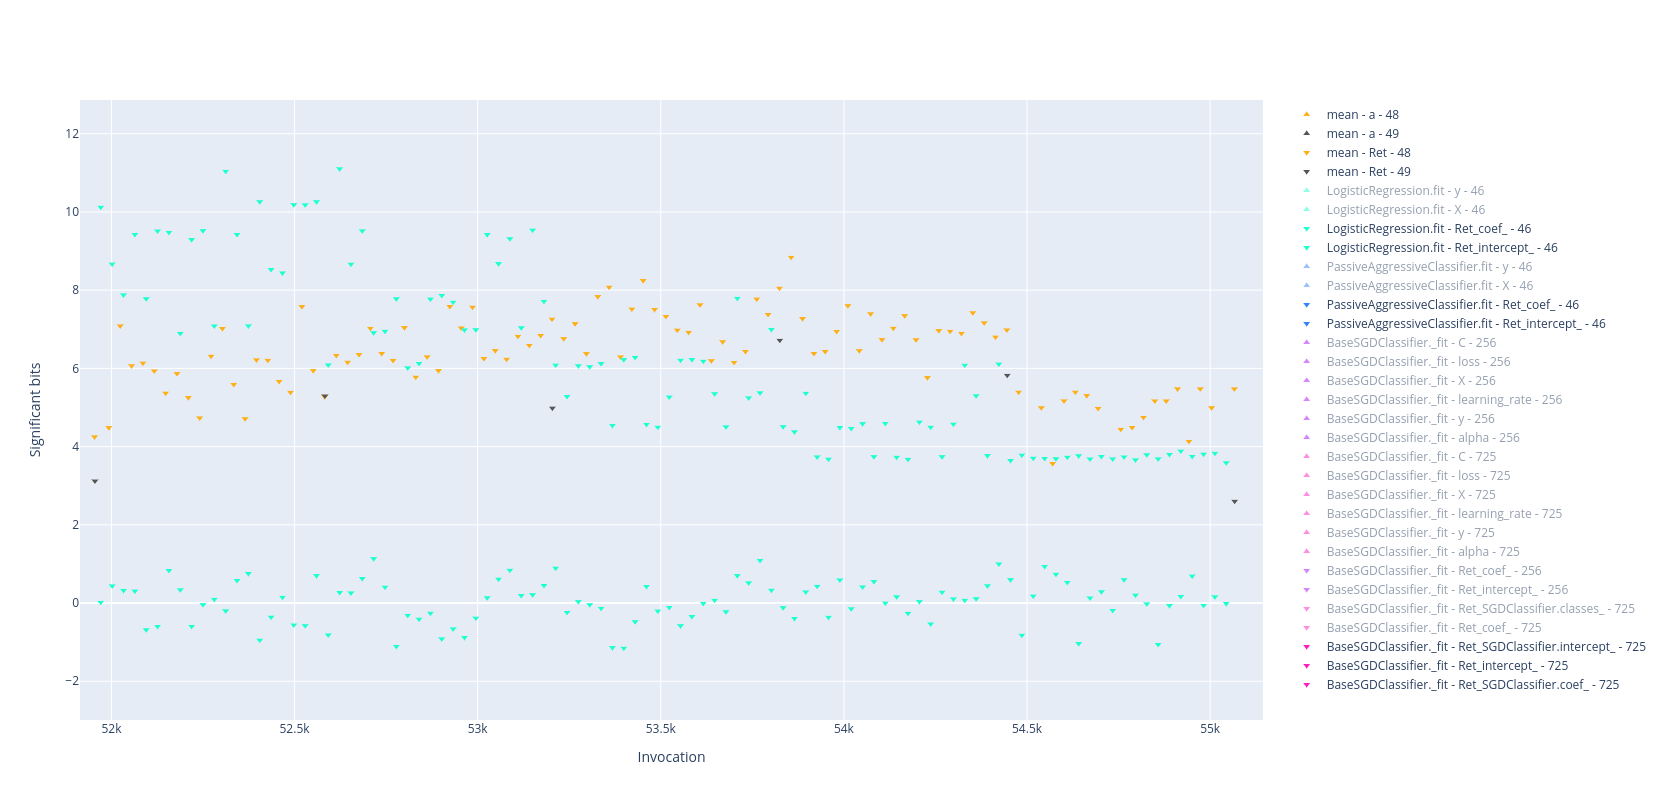
\includegraphics[width=\linewidth]{figure/classifier_comparisons/SAG_predicition_s.png}
%     \caption{Number of significant digits (General view).}
%     \label{fig:classifier_comparisons_general}
% \end{figure}

% \begin{figure}
%     \centering
%     \caption{Caption}
%     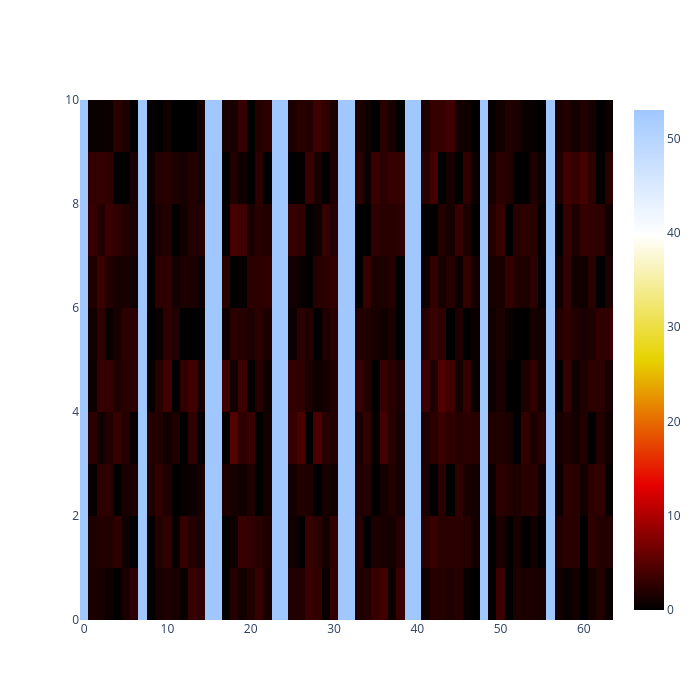
\includegraphics[width=\linewidth]{figure/classifier_comparisons/zoom_SAG_fit_coef_s.png}
%     \caption{Number of significant digits (General view).}
%     \label{fig:classifier_comparisons_general}
% \end{figure}


% \subsubsection{Adaboost}
\paragraph{Adaboost}
This test compare a decision trees boosted with 300 estimators using the AdaBoost.R2~\cite{drucker1997improving} algorithm with
a single decision tree regressor on a 1D sinusoidal dataset with a small amount of Gaussian noise. 
The depth is fixed at 4. 
% The example shows that as the number of boosts is increased the regressor can fit more detail.

% RR Good 48 \\
% MCA: arange issue /  bootstrap\_idx = random\_state.choice(a=np.arange(\_num\_samples(X)), size=\_num\_samples(X), replace=True, p=sample\_weight) / len(a) != len(p)

\paragraph{Online classifier comparison}

This example compares how the following online solvers perform on the hand-written digits dataset:
Stochastic Gradient Descent (SGD) with maximum iterations fixed to 100, 
Averaged Stochastic Gradient Descent (ASGD),
Perceptron, Passive-Aggressive I with the hinge loss function, tolerance 
and regularization fixed at $10^{-4}$ and $1$,
Passive-Aggressive II with the squared hinge loss function, tolerance 
and regularization fixed at $10^{-4}$ and $1$, and Stochastic Average Gradient (SAG)
with the tolerance and regularization fixed at $10^{-4}$ and $5.10^{-8}$.

% RR: stable 48 bits. \\
% MCA: Index issue

\paragraph{Bayesian Ridge Regression}

This test compares a Bayesian Ridge Regression (BRR) to the Ordinary Least Squares (OLS) estimator on a synthetic dataset and for one-dimensional regression using polynomial feature expansion. Although the test does not raise a runtime error, the coefficients computed from the fitting for the synthetic dataset are \texttt{Not-A-Number} (NaN) values for both BRR and OLS. \pytracer traces reveal that the SVD solver used is the root cause. Figure~\ref{fig:brr_svd_sig} shows
the number of significant bits for the singular values SVD decomposition 
For BRR, the SVD is directly called to compute the coefficient, while for the OLS, it is called during the Least-Squares minimization. Scikit-learn uses SciPy that itself uses the LAPACK library to compute the SVD.
The LAPACK library has two main methods for computing the SVD: 
\texttt{gesdd} and \texttt{gesvd}. The first one uses a Divide \& Conquer approach, while the second uses a QR decomposition. While both methods expect to have the same accuracy~\cite{nakatsukasa2013stable}, it appears that results diverge in practice with inaccurate results for the Divide \& Conquer method, as the sill opened an issue on the official LAPACK GitHub repository \href{https://github.com/Reference-LAPACK/lapack/issues/316}{github.com/Reference-LAPACK/lapack/issues/316} shows. For the Least-Square problem, the LAPACK library has three solvers, including \texttt{dgelss} that internally uses \texttt{gesdd} and \texttt{dgelsd} that uses \texttt{gesvd}. By using the \texttt{gesvd} (dgelsd) method instead of the \texttt{gesdd} (dgelss) one, the SVD is converging within the RR and Full MCA modes, with a number of significant bits of 44 on average.

\begin{figure}
    \centering
    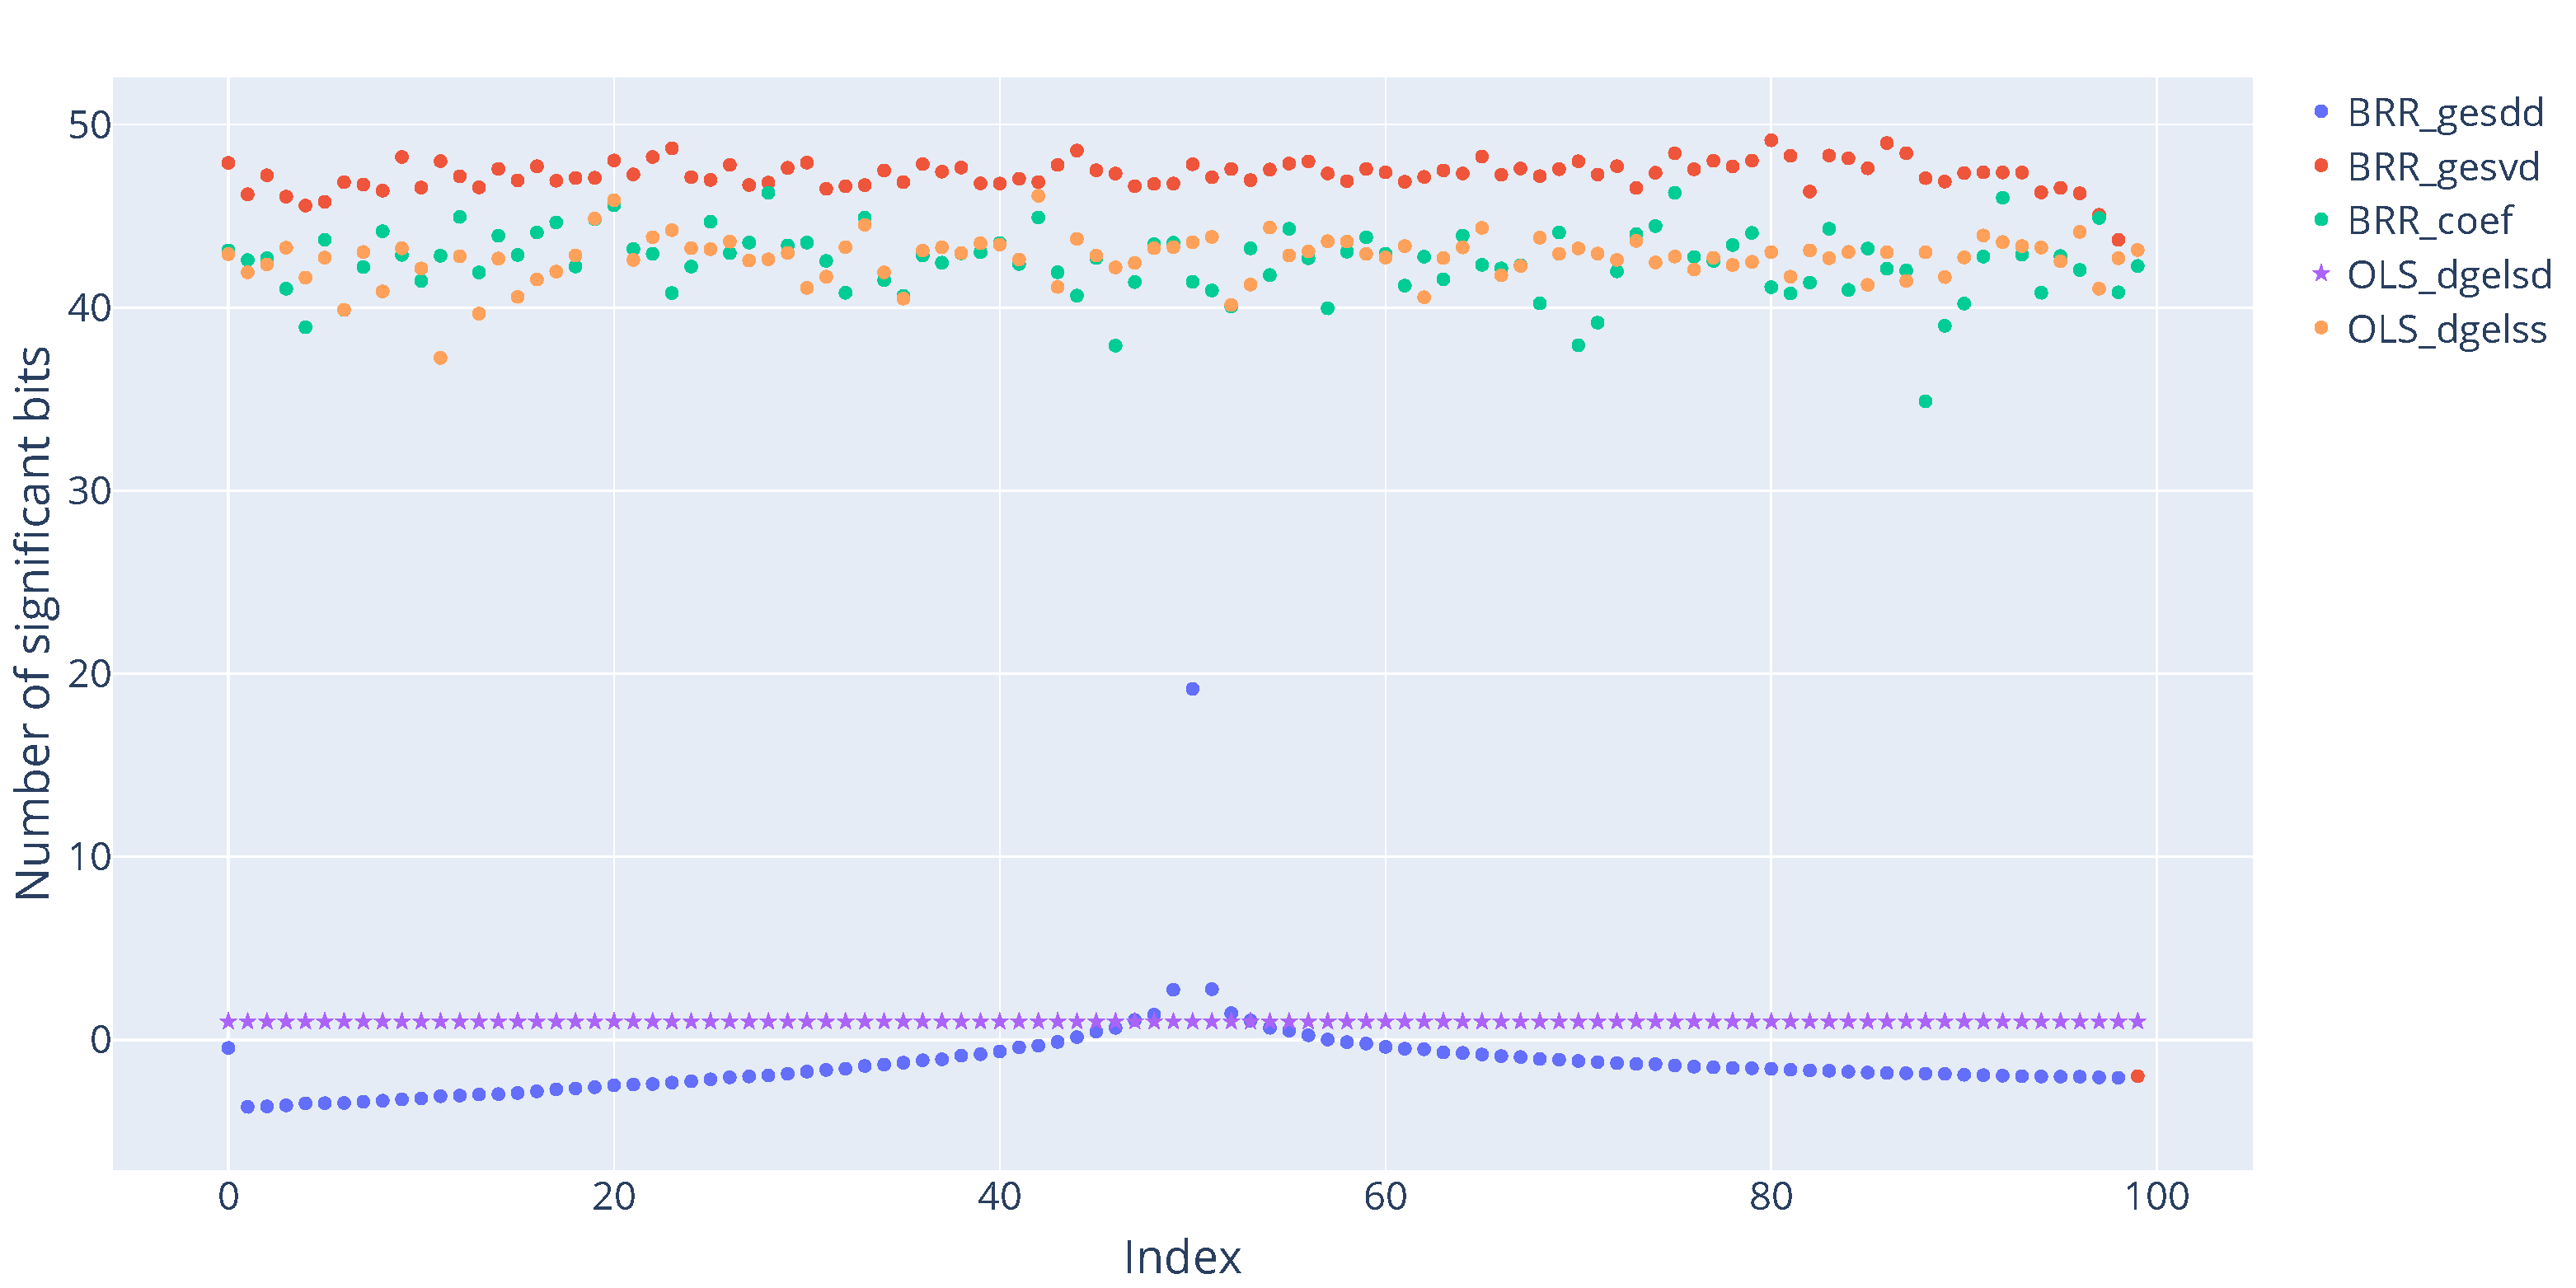
\includegraphics[width=\linewidth]{figure/BRR/BRR_coefs_sig.pdf}
    \caption{Bayesian Ridge Regression coefficients within RR mode.
    The \texttt{BRR\_*} points show the \texttt{BayesianRidge} results
    using the \texttt{gesdd} and \texttt{gesvd} methods. 
    The \texttt{OLS\_*} points show the \texttt{LinearRegression} results
    with the \texttt{dgelsd} and \texttt{dgelss} methods.
    We can see that using the Divide \& Conquer method for the SVD
    (\texttt{gesdd} and  \texttt{dgelsd})
    gives very low precision
    results for \textit{BRR} and even \texttt{NaN} values (star points) for \textit{OLS}. By switching to the \texttt{gesvd} method, 
    results have a precision of 42 bits in average.
    }
    \label{fig:brr_svd_sig}
\end{figure}

% the coefficient weights are slightly shifted toward zeros, which stabilises them.
% As the prior on the weights is a Gaussian prior, the histogram of the estimated weights is Gaussian.
% The estimation of the model is done by iteratively maximizing the marginal log-likelihood of the observations.
% We also plot predictions and uncertainties for Bayesian Ridge Regression for one dimensional regression using polynomial feature expansion. Note the uncertainty starts going up on the right side of the plot. This is because these test samples are outside of the range of the training samples.

% RR: solution mean 15-24 / std 20-30 \\
% MCA: SVD did not converge

\paragraph{K-Means Clustering}

This test uses the K-means to cluster the IRIS dataset.
% The plots display firstly what a K-means algorithm would yield using three clusters. It is then shown what the effect of a bad initialization is on the classification process: By setting n\_{init} to only 1 (default is 10), the amount of times that the algorithm will be run with different centroid seeds is reduced. The next plot displays what using eight clusters would deliver and finally the ground truth.

% RR Very stable (labels with highest precision) \\
% MCA: Divergence

\paragraph{Covariance estimation}

This example shows covariance estimation with Mahalanobis distances on Gaussian distributed data.

% For Gaussian distributed data, the distance of an observation xi to the mode of the distribution can be computed using its Mahalanobis distance:

% d(μ,Σ)(xi)2=(xi−μ)TΣ−1(xi−μ)
% where μ and Σ are the location and the covariance of the underlying Gaussian distributions.

% In practice, μ and Σ are replaced by some estimates. The standard covariance maximum likelihood estimate (MLE) is very sensitive to the presence of outliers in the data set and therefore, the downstream Mahalanobis distances also are. It would be better to use a robust estimator of covariance to guarantee that the estimation is resistant to “erroneous” observations in the dataset and that the calculated Mahalanobis distances accurately reflect the true organization of the observations.

% The Minimum Covariance Determinant estimator (MCD) is a robust, high-breakdown point (i.e. it can be used to estimate the covariance matrix of highly contaminated datasets, up to 
 
% nsamples−nfeatures−12 outliers) estimator of covariance. The idea behind the MCD is to find 
 
% nsamples+nfeatures+12 observations whose empirical covariance has the smallest determinant, yielding a “pure” subset of observations from which to compute standards estimates of location and covariance. The MCD was introduced by P.J.Rousseuw in 1.

% This example illustrates how the Mahalanobis distances are affected by outlying data. Observations drawn from a contaminating distribution are not distinguishable from the observations coming from the real, Gaussian distribution when using standard covariance MLE based Mahalanobis distances. Using MCD-based Mahalanobis distances, the two populations become distinguishable. Associated applications include outlier detection, observation ranking and clustering.



% RR: Traces diverge but precision seems stable (~48bits) \\
% Main computation is in a loop that might be take extra steps to ends. \\
% MCA: arange issue

\paragraph{Decision Tree Regression}

This test uses a decision tree to fit a sine curve with added noise.

% A 1D regression with decision tree.
% The decision trees is used to fit a sine curve with addition noisy observation. As a result, it learns local linear regressions approximating the sine curve.
% We can see that if the maximum depth of the tree (controlled by the max\_depth parameter) is set too high, the decision trees learn too fine details of the training data and learn from the noise, i.e. they overfit.


% RR Fit ok (50bits) , missing predict \\
% MCA Fit ok (50bits) , missing predict

\paragraph{Digits Classification}

This test uses a Support Vector Classifier to recognize images of hand-written
digits. The digits dataset consists of 8x8 pixel images of digits

% RR Very stable (highest precision) \\
% MCA: Very stable (highest precision)

\paragraph{Face Recognition}

The face recognition test uses eigenfaces (eigenvector) and Support Vector Machines (SVMs) to classify faces from the Labeled Faces in the Wild dataset~\cite{LFWTech}. This test uses a Principal Component Analysis (PCA) to extract the eigenfaces and then trains an SVM classifier to predict the name associated with a visage. This test is the only one to raise an error within RR mode due to a non-convergence of the Singular Value Decomposition (SVD) performed during the PCA.
In this test, the PCA uses the Randomized SVD~\cite{halko2011finding} variant that first computes a low-rank approximation of the input matrix by using a stochastic algorithm and then uses this approximation as the input for the SVD. It is during the computation of this SVD that the test raised an error.

Scikit-learn uses SciPy that itself uses the LAPACK library to compute the SVD. The LAPACK library has two main methods for computing the SVD: 
\texttt{gesdd} and \texttt{gesvd}. The first one uses a Divide \& Conquer approach, while the second uses a QR decomposition. While both methods expect to have the same accuracy~\cite{nakatsukasa2013stable}, it appears that results diverge in practice with inaccurate results for the Divide \& Conquer method, as the sill opened an issue on the official LAPACK GitHub repository \href{https://github.com/Reference-LAPACK/lapack/issues/316}{github.com/Reference-LAPACK/lapack/issues/316} shows. The \texttt{randomized\_svd} scikit-learn function uses the Divide \& Conquer method for the SVD. 

By using the \texttt{gesvd} method instead of the \texttt{gesdd} one, the SVD is converging within the RR mode. Moreover, figure~\ref{fig:randomized_svd_S} shows the precision of the eigenvalues computed, varying between 15 and 20 bits out of the 24 available in single precision. Finally, the classifier metrics (precision, recall, F1-score, and support) are identical to the IEEE execution, meaning that the test is as precise as the original execution.

In conclusion, the MCA model was helpful to detect the instability of the \texttt{gesdd} method that has been notified in several GitHub issues, including the LAPACK repository. It is worth mentioning that recently, a Pull Request has been submitted to let the user select the SVD method and avoid this kind of issue.

\begin{figure}
    \centering
    \begin{subfigure}{0.3\linewidth}
    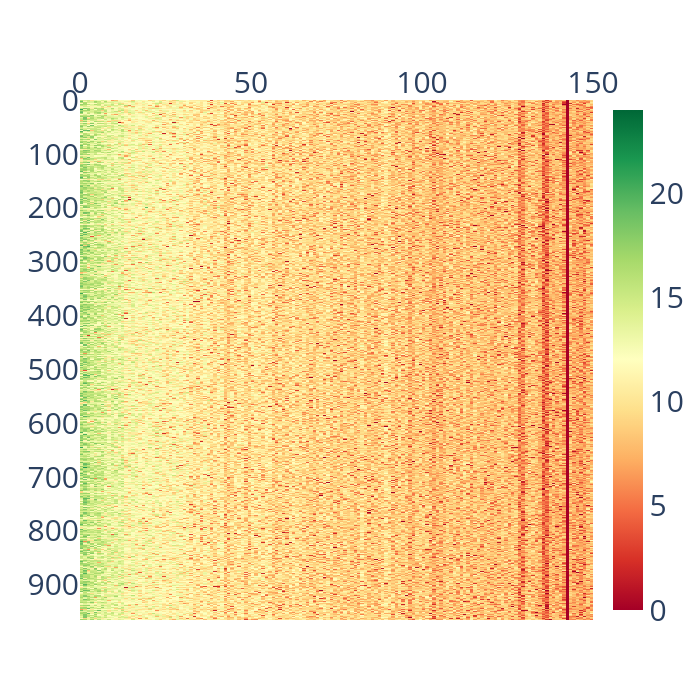
\includegraphics[width=\linewidth]{figure/face_recognition/randomized_svd_ret_U_sig_zoom.png}
    \caption{Left matrix $U$ of the SVD decomposition}
    \label{fig:randomized_svd_U}
    \end{subfigure}
    \begin{subfigure}{0.3\linewidth}
    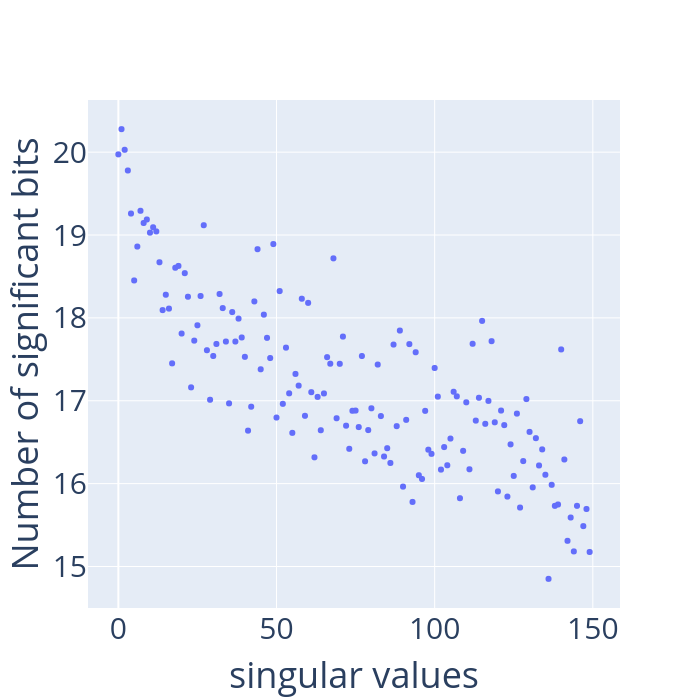
\includegraphics[width=\linewidth]{figure/face_recognition/randomized_svd_ret_S_sig.png}
    \caption{Singular values $\Sigma$ of the SVD decomposition}
    \label{fig:randomized_svd_S}
    \end{subfigure}
    \begin{subfigure}{0.3\linewidth}
    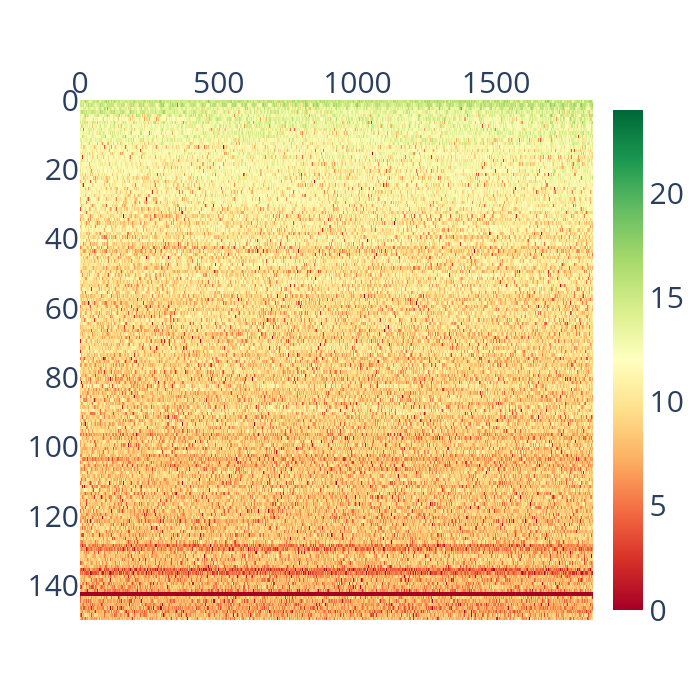
\includegraphics[width=\linewidth]{figure/face_recognition/randomized_svd_ret_V_sig_zoom.png}
    \caption{Right matrix $V$ of the SVD decomposition}
    \label{fig:randomized_svd_V}
    \end{subfigure}
    \caption{Number of significant bits of the \texttt{randomized\_svd} function in the 
    \texttt{face\_recognition} test using the \texttt{gesvd} SVD method within RR mode.
    Figures~\ref{fig:randomized_svd_U},~\ref{fig:randomized_svd_S}, and~\ref{fig:randomized_svd_V}
    show respectively the values $U$, $\Sigma$ and $V.$
    Using this method makes the \texttt{randomized\_svd} converging contrary to the \texttt{gesdd} method that raised a runtime error. 
    }
    \label{fig:face_recognition_svd}
\end{figure}

% RR: Crash due to FP32 use. Does FP64 converge? No. Does sgsvd converge? Yes

% MCA: arange issue

% File "/usr/local/lib/python3.8/site-packages/sklearn/datasets/\_lfw.py", line 169, in \_load\_imgs
%     faces[i, ...] = face
% ValueError: could not broadcast input array from shape (49,37) into shape (50,37)

\paragraph{L1 Penalty}

This test compares the percentage of zero coefficients for logistic regression
by varying the penalty (L1, L2 and Elastic-Net) and regularization (1, 0.1, 0.01) parameters. Large regularization value gives more freedom to the model
while small value puts more constraints on the model.

% of L1, L2 and Elastic-Net penalty.

% Comparison of the sparsity (percentage of zero coefficients) of solutions when L1, L2 and Elastic-Net penalty are used for different values of C. We can see that large values of C give more freedom to the model. Conversely, smaller values of C constrain the model more. In the L1 penalty case, this leads to sparser solutions. As expected, the Elastic-Net penalty sparsity is between that of L1 and L2.
% We classify 8x8 images of digits into two classes: 0-4 against 5-9. The visualization shows coefficients of the models for varying C.

% RR: ok \\
% MCA: stable for L1 and L2, not for Len but coef have less zeroes. 


\paragraph{Lasso and Elastic-Net}


This test compares the Lasso and Elastic-Net regression models
on a corrupted signal.

% Estimates Lasso and Elastic-Net regression models on a manually generated sparse signal corrupted with an additive noise. Estimated coefficients are compared with the ground-truth.

% RR: Good (48 bits on coefs) \\
% MCA: Good like RR if we exclude one trace that fails due to arange issue

\paragraph{Separating hyperplane}

This test uses a linear Support Vector Machine (SVM) classifier trained using the Stochastic Gradient Descent (SGD) method to find the maximum separating hyperplane in 2D.
The test trains the SVM with 50 random points separated in 2 clusters with hyperparameters $\alpha=0.01$ and using the hinge loss function. Once trained, the test generates a $[-1,5]\times[-1,5]$ Cartesian grid and predicts the class label for each point with integer coordinates. Figure~\ref{fig:separating_hyperplan} shows the ratio $\frac{mean}{std}$ with RR mode for each point of the grid (square) and the training dataset (circle), the two colors representing the two classes.
We can see that white points close to the separating hyperplane are highly unstable with a number of significant bits below 0, meaning that
the classifier hesitates about the class to predict.


% \begin{figure}
%     \centering
%     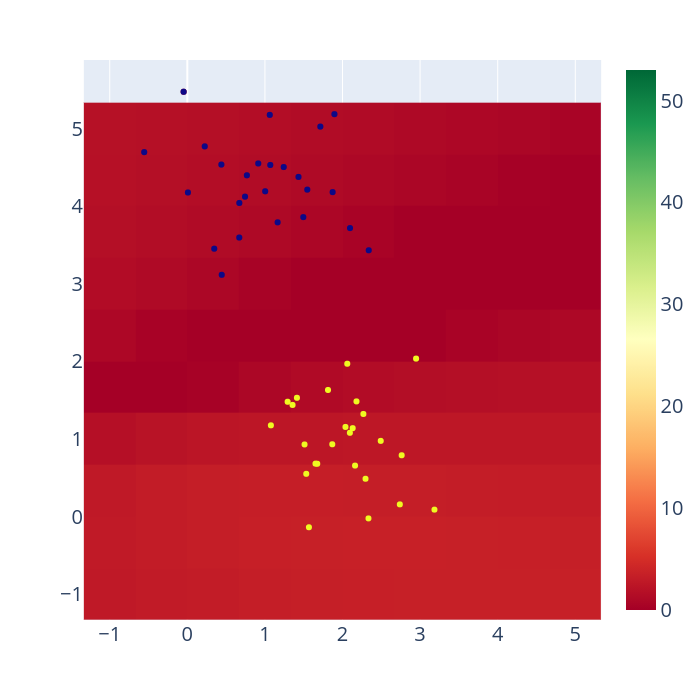
\includegraphics[width=\linewidth]{figure/separating_hyperplan/hyperplan.png}
%     \caption{Ratio $mean/std$ of Separating hyperplane test result within RR mode.
%     Circle and square points represent respectively the train and test dataset.
%     The color represents the predicted class. We can see that 
%     instability is high around the hyperplane which is coherent with 
%     the fact the classifier has difficulty to decide in which side of the hyperplane the 
%     point is.}
%     \label{fig:separating_hyperplan}
% \end{figure}

\begin{figure}
    \centering
    \begin{subfigure}{.3\linewidth}
    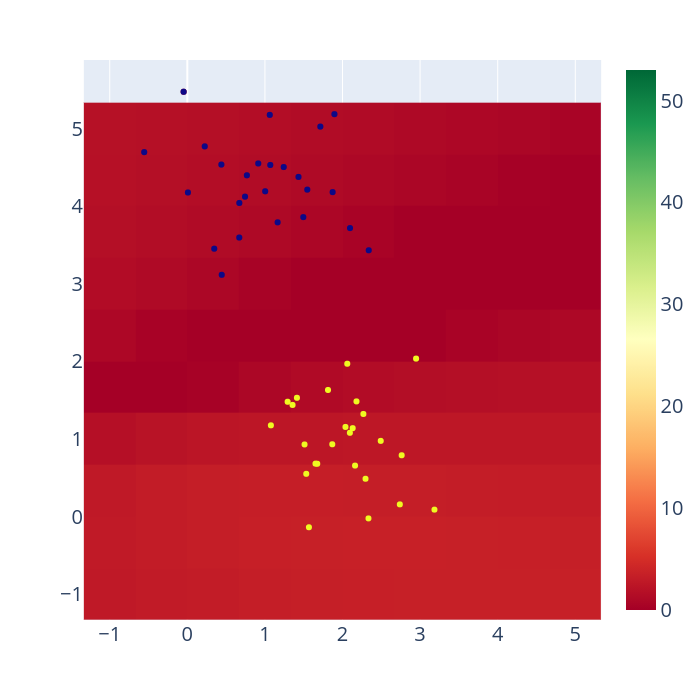
\includegraphics[width=\linewidth]{figure/separating_hyperplan/hyperplan.png}
    \caption{}
    \label{fig:hyperplan_sig}
    \end{subfigure}
    \begin{subfigure}{.3\linewidth}
    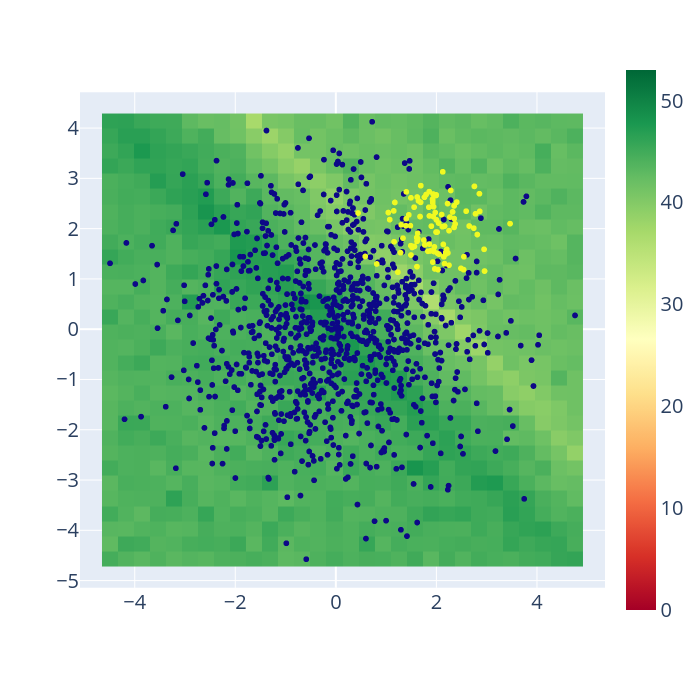
\includegraphics[width=\linewidth]{figure/SVM/non_weighted.png}
    \caption{}
    \label{fig:SVM_nw_sig}
    \end{subfigure}
    \begin{subfigure}{.3\linewidth}
    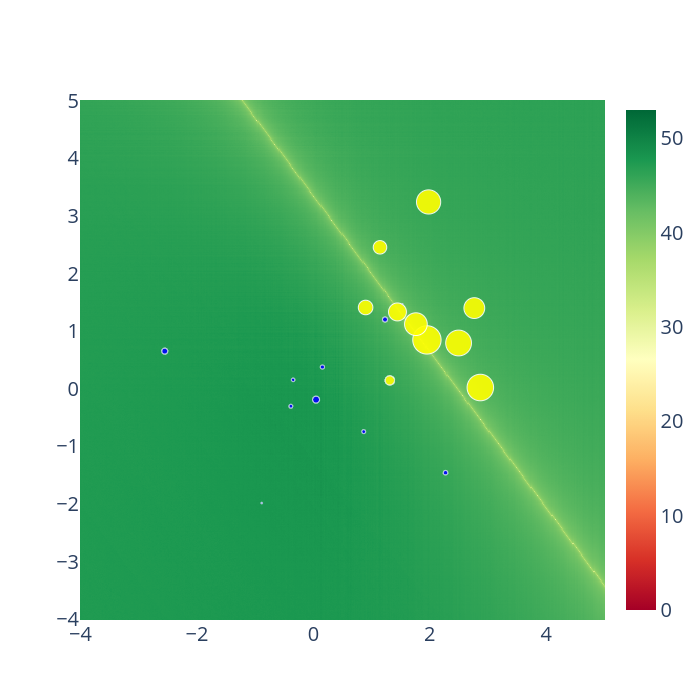
\includegraphics[width=\linewidth]{figure/Weighted/non_weighted.png}
    \caption{}
    \label{fig:weighted_nw_sig}
    \end{subfigure}
    \begin{subfigure}{.3\linewidth}
    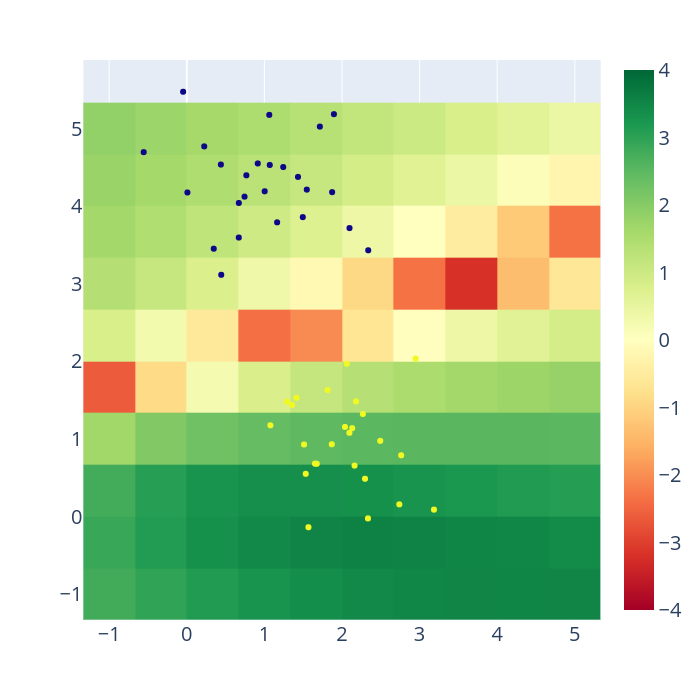
\includegraphics[width=\linewidth]{figure/separating_hyperplan/hyperplan_zoom.png}
    \caption{}
    \label{fig:hyperplan_sig_zoom}
    \end{subfigure}
    \begin{subfigure}{.3\linewidth}
    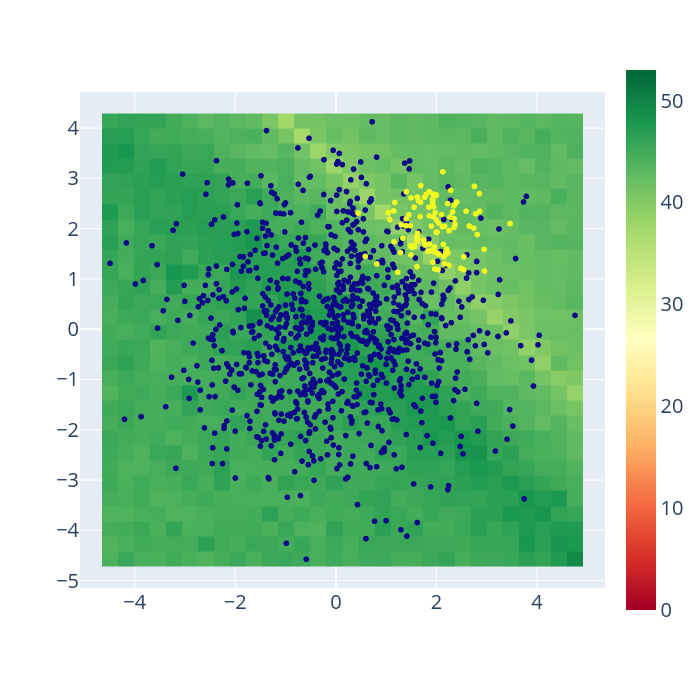
\includegraphics[width=\linewidth]{figure/SVM/weighted.png}
    \caption{}
    \label{fig:SVM_w_sig}
    \end{subfigure}
    \begin{subfigure}{.3\linewidth}
    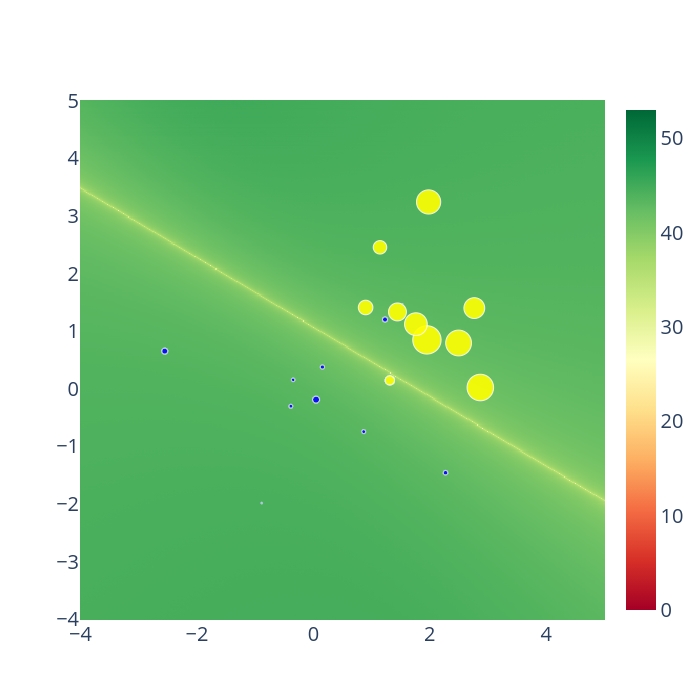
\includegraphics[width=\linewidth]{figure/Weighted/weighted.png}
    \caption{}
    \label{fig:weighted_w_sig}
    \end{subfigure}
    \caption{Three examples of separating hyperplane tests.  All figures show the number of significant bits of the results for the following tests: \textit{Separating Hyperplane} on figures.~\ref{fig:hyperplan_sig} for the original colormap and~\ref{fig:hyperplan_sig_zoom} with a rescaled colormap. We can see that this test exhibits a poor precision with less than 3 bits significant, although only the sign of the number matter to predict on which side of the hyperplane the point is classified.
We can see in figure~\ref{fig:hyperplan_sig_zoom} by rescaling the colormap that the instabilities are concentrated around the hyperplane.
    Figures~\ref{fig:SVM_nw_sig},~\ref{fig:SVM_w_sig},~\ref{fig:weighted_nw_sig}, and~\ref{fig:weighted_w_sig} show respectively the results of tests    \textit{SVM} and~\textit{Weighted samples}. Figures~\ref{fig:SVM_nw_sig} and~\ref{fig:weighted_nw_sig} show the unweighted classification while figures~\ref{fig:SVM_w_sig} and~\ref{fig:weighted_nw_sig} the classification taking into account the weights. We can see that taking into account the weight classes allows a better separating.}
\label{fig:my_label}
\end{figure}

\paragraph{MNIST classification}

This test fits a logistic regression with the SAGA solver with the L1 penalty  
on a subset of the MNIST digits classification task.

% Here we fit a multinomial logistic regression with L1 penalty on a subset of the MNIST digits classification task. We use the SAGA algorithm for this purpose: this a solver that is fast when the number of samples is significantly larger than the number of features and is able to finely optimize non-smooth objective functions which is the case with the l1-penalty. Test accuracy reaches > 0.8, while weight vectors remains sparse and therefore more easily interpretable.
% Note that this accuracy of this l1-penalized linear model is significantly below what can be reached by an l2-penalized linear model or a non-linear multi-layer perceptron model on this dataset.

% RR: Very stable \\
% MCA: Parse by excluding a trace that failed due to an arange issue

\paragraph{Multitask Lasso}

This test compares the Lasso and MultiTaskLasso regression models
on a corrupted signal.

% The multi-task lasso allows to fit multiple regression problems jointly enforcing the selected features to be the same across tasks. This example simulates sequential measurements, each task is a time instant, and the relevant features vary in amplitude over time while being the same. The multi-task lasso imposes that features that are selected at one time point are select for all time point. This makes feature selection by the Lasso more stable.

% RR: Stable (44~53 bits for coef) \\
% MCA: Stable like RR if we exclude a trace that failed due index issue

\paragraph{Orthogonal matching}

This test uses the Orthogonal Matching Pursuit algorithm
for recovering a sparse signal from a noisy measurement encoded with a dictionary.

% RR: Very stable \\
% MCA: Very stable

\paragraph{PCA decomposition}

This test makes a PCA decomposition on a synthetic dataset.
% These figures aid in illustrating how a point cloud can be very flat in one direction–which is where PCA comes in to choose a direction that is not flat.

% rr: stable (48 bits on components) \\
% mca: stable (48 bits on components)

\paragraph{Robust Linear Regression}

This test compare the linear and  RANSAC regression methods on a noisy data.
% In this example we see how to robustly fit a linear model to faulty data using the RANSAC algorithm.   


% RR: Very stable \\
% MCA: Very stable if we exclude two traces that failed due to arange/index issues

\paragraph{Segmentation Toy}

This test uses a spectral clustering to separate connected circles in an image.

% In this example, an image with connected circles is generated and spectral clustering is used to separate the circles.

% In these settings, the Spectral clustering approach solves the problem know as ‘normalized graph cuts’: the image is seen as a graph of connected voxels, and the spectral clustering algorithm amounts to choosing graph cuts defining regions while minimizing the ratio of the gradient along the cut, and the volume of the region.

% As the algorithm tries to balance the volume (ie balance the region sizes), if we take circles with different sizes, the segmentation fails.

% In addition, as there is no useful information in the intensity of the image, or its gradient, we choose to perform the spectral clustering on a graph that is only weakly informed by the gradient. This is close to performing a Voronoi partition of the graph.

% In addition, we use the mask of the objects to restrict the graph to the outline of the objects. In this example, we are interested in separating the objects one from the other, and not from the background.

% RR Stable \\
% MCA: Stable if we exclude three traces that failed due to index issue

\paragraph{SVM}

This test uses an plain and weighted classes SVC to find the best hyperplan separating an unbalanced dataset.

% Find the optimal separating hyperplane using an SVC for classes that are unbalanced.

% We first find the separating plane with a plain SVC and then plot (dashed) the separating hyperplane with automatically correction for unbalanced classes.

% RR: stable (48 bits) \\
% MCA: stable (48 bits)

\paragraph{Tomography}

This test compares the LASSO and Ridge regression models to 
reconstruct an image from a set of projections for a dataset
acquired from computed tomography.

% This test shows the reconstruction of an image from a set of parallel projections, acquired along different angles. Such a dataset is acquired in computed tomography (CT). 

% Without any prior information on the sample, the number of projections required to reconstruct the image is of the order of the linear size l of the image (in pixels). For simplicity we consider here a sparse image, where only pixels on the boundary of objects have a non-zero value. Such data could correspond for example to a cellular material. Note however that most images are sparse in a different basis, such as the Haar wavelets. Only l/7 projections are acquired, therefore it is necessary to use prior information available on the sample (its sparsity): this is an example of compressive sensing.

% The tomography projection operation is a linear transformation. In addition to the data-fidelity term corresponding to a linear regression, we penalize the L1 norm of the image to account for its sparsity. The resulting optimization problem is called the Lasso. We use the class Lasso, that uses the coordinate descent algorithm. Importantly, this implementation is more computationally efficient on a sparse matrix, than the projection operator used here.

% The reconstruction with L1 penalization gives a result with zero error (all pixels are successfully labeled with 0 or 1), even if noise was added to the projections. In comparison, an L2 penalization (Ridge) produces a large number of labeling errors for the pixels. Important artifacts are observed on the reconstructed image, contrary to the L1 penalization. Note in particular the circular artifact separating the pixels in the corners, that have contributed to fewer projections than the central disk.

% RR Divergence \\
% MCA Index issue

\paragraph{Weighted samples}

This test uses a SGD to separate weighted points by 
taking into account or the not the weights.


% RR Stable (30~48 bits on coef) \\
% MCA Unstable (0 bits on coef)

\subsection{PyAFQ}


PyAFQ is Python package for Automated Fiber Quantification.
It aims at finding delineation of the major fiber tracts in individual human brains, and quantification of the tissue properties within the tracts.

\section{Performance evaluation}

In this section, we review the performance overhead of the Pytracer's instrumentation cost
and the time spent during the postprocessing analysis. 

\subsection{Tracing}

Pytracer instrumentation overhead comes from the time spent to instrument module (initialization overhead)
before executing the targeted application plus the cost for dumping the data during the execution (running overhead).
The initialization overhead is proportional the number of functions and classes traced. 
However, initialization overhead is amortized when traced applications are above 8 seconds, which is proportional to 
the number of functions and classes traced.
Table~\ref{tab:pytracer_overhead} summaries the slowdown measure on SciPy
and scikit-learn tests.
We can see that Pytracer gives slowdown of $\times 17$ and
$\times 3.5$ if we subtract the initialization step.
By adding fuzzy, we have an average slowdown of $\times 37$ for RR mode and $\times 43$ for Full MCA.

\begin{figure}
    \centering
    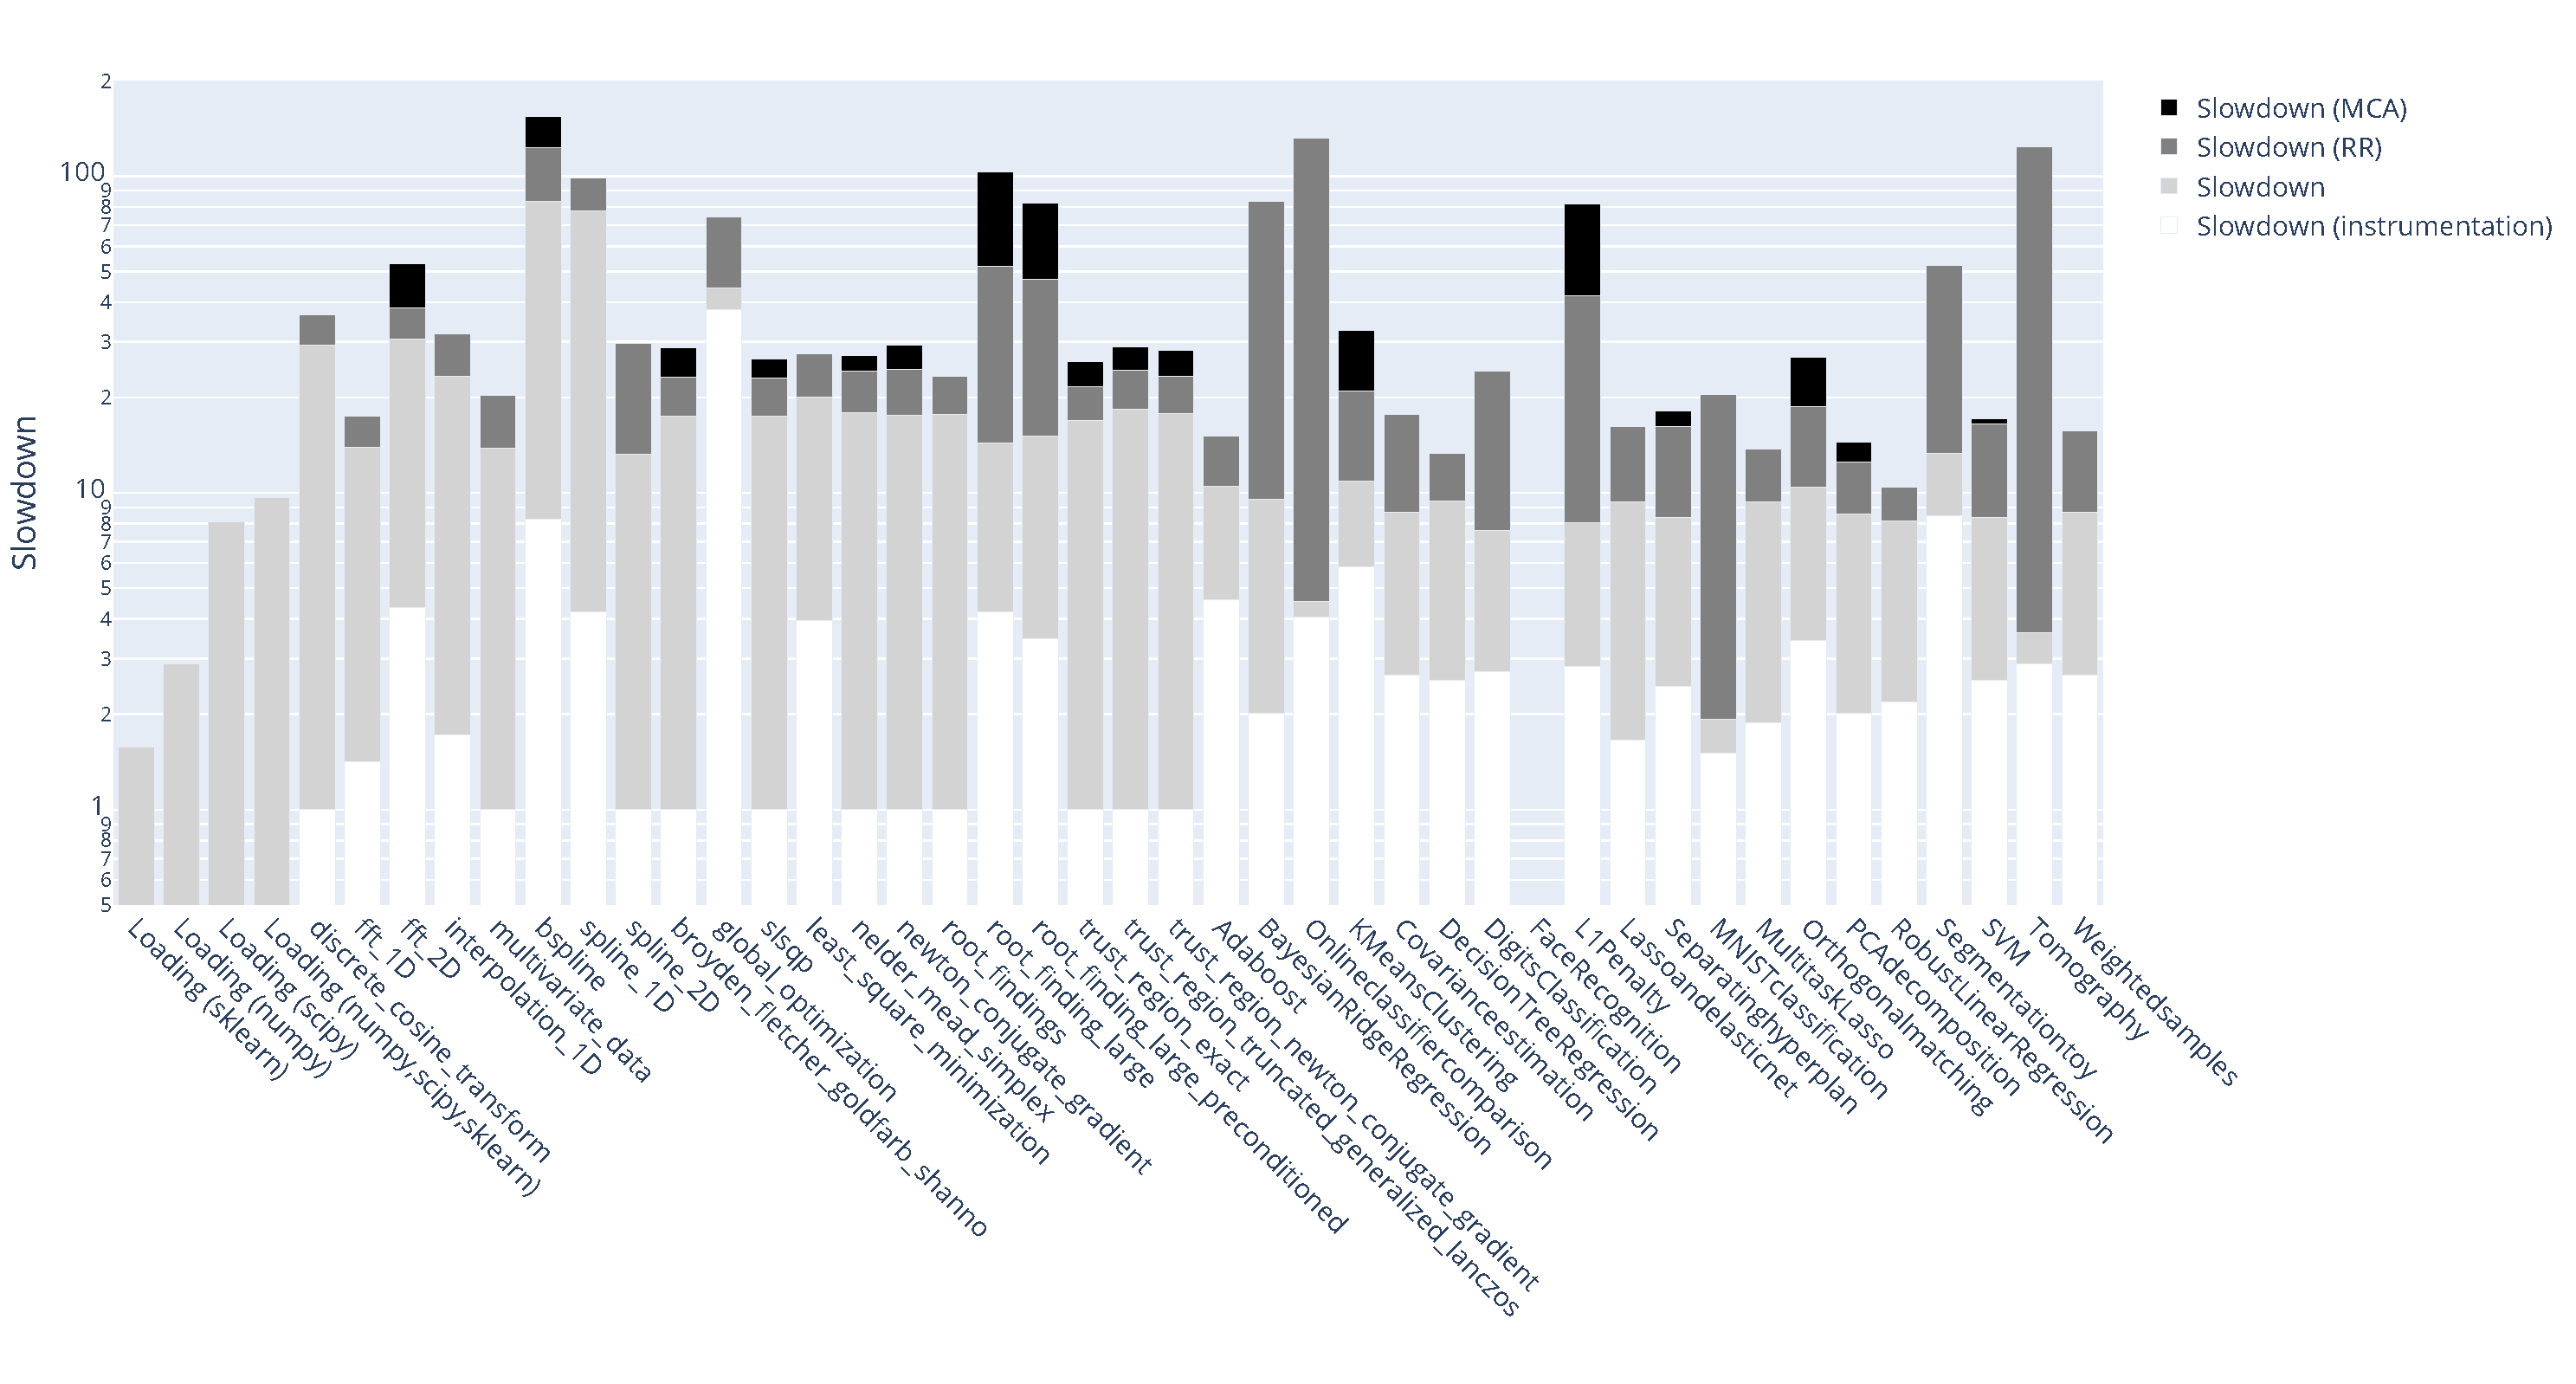
\includegraphics[width=\linewidth]{figure/performance.pdf}
    \caption{
    The figure presents the \pytracer tracing overheads: \textit{Slowdown} is the actual overhead, computed as the ratio between the execution time without and with \pytracer. This slowdown can be high for the tests running less than 8 seconds because \pytracer spends most of its time in the initialization step. Since this step is a constant factor of the number of functions instrumented, we also plot the slowdown of the instrumentation itself (\textit{Slowdown (Instrumentation)} calculated by subtracting the initialization time.
    The \textit{Slowdown (RR)} and \textit{Slowdown (MCA)} colors show the slowdown of \pytracer 
    using the fuzzy environment with RR and Full MCA modes.
    The first four tests measure the initialization steps depending on the modules instrumented.
    }
    \label{fig:performances}
\end{figure}

\begin{figure}
    \centering
    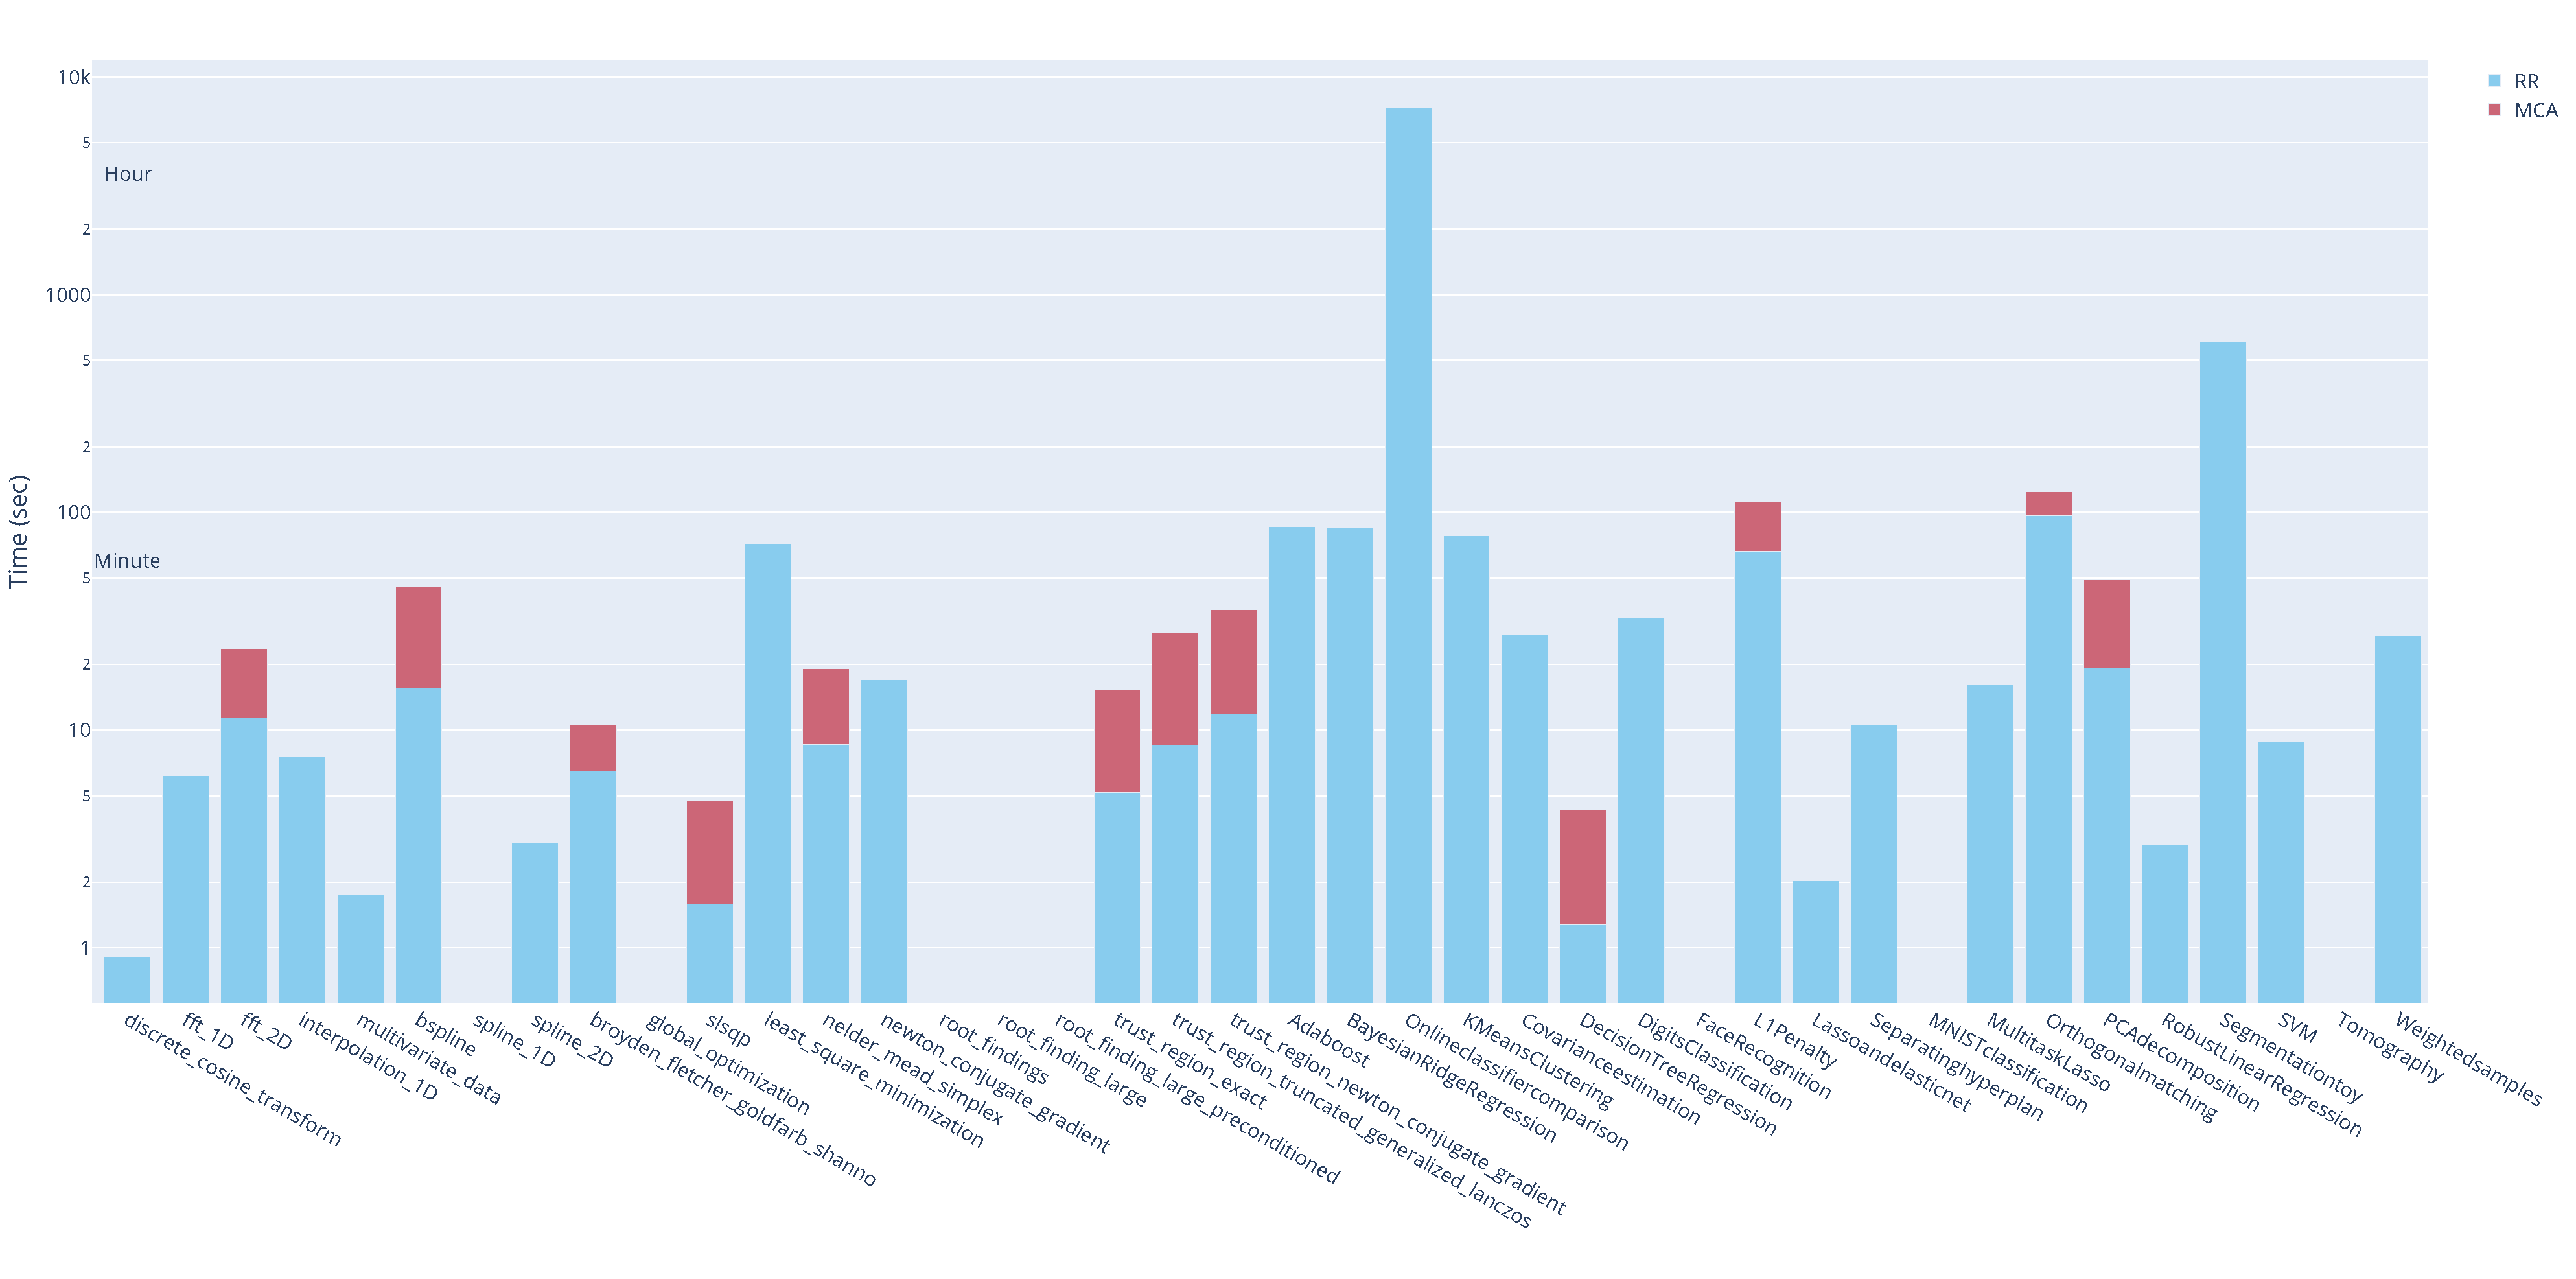
\includegraphics[width=\linewidth]{figure/parsing_time.pdf}
    \caption{\pytracer time to aggregate traces.}
    \label{fig:performance_parsing_time}
\end{figure}

\begin{figure}
    \centering
    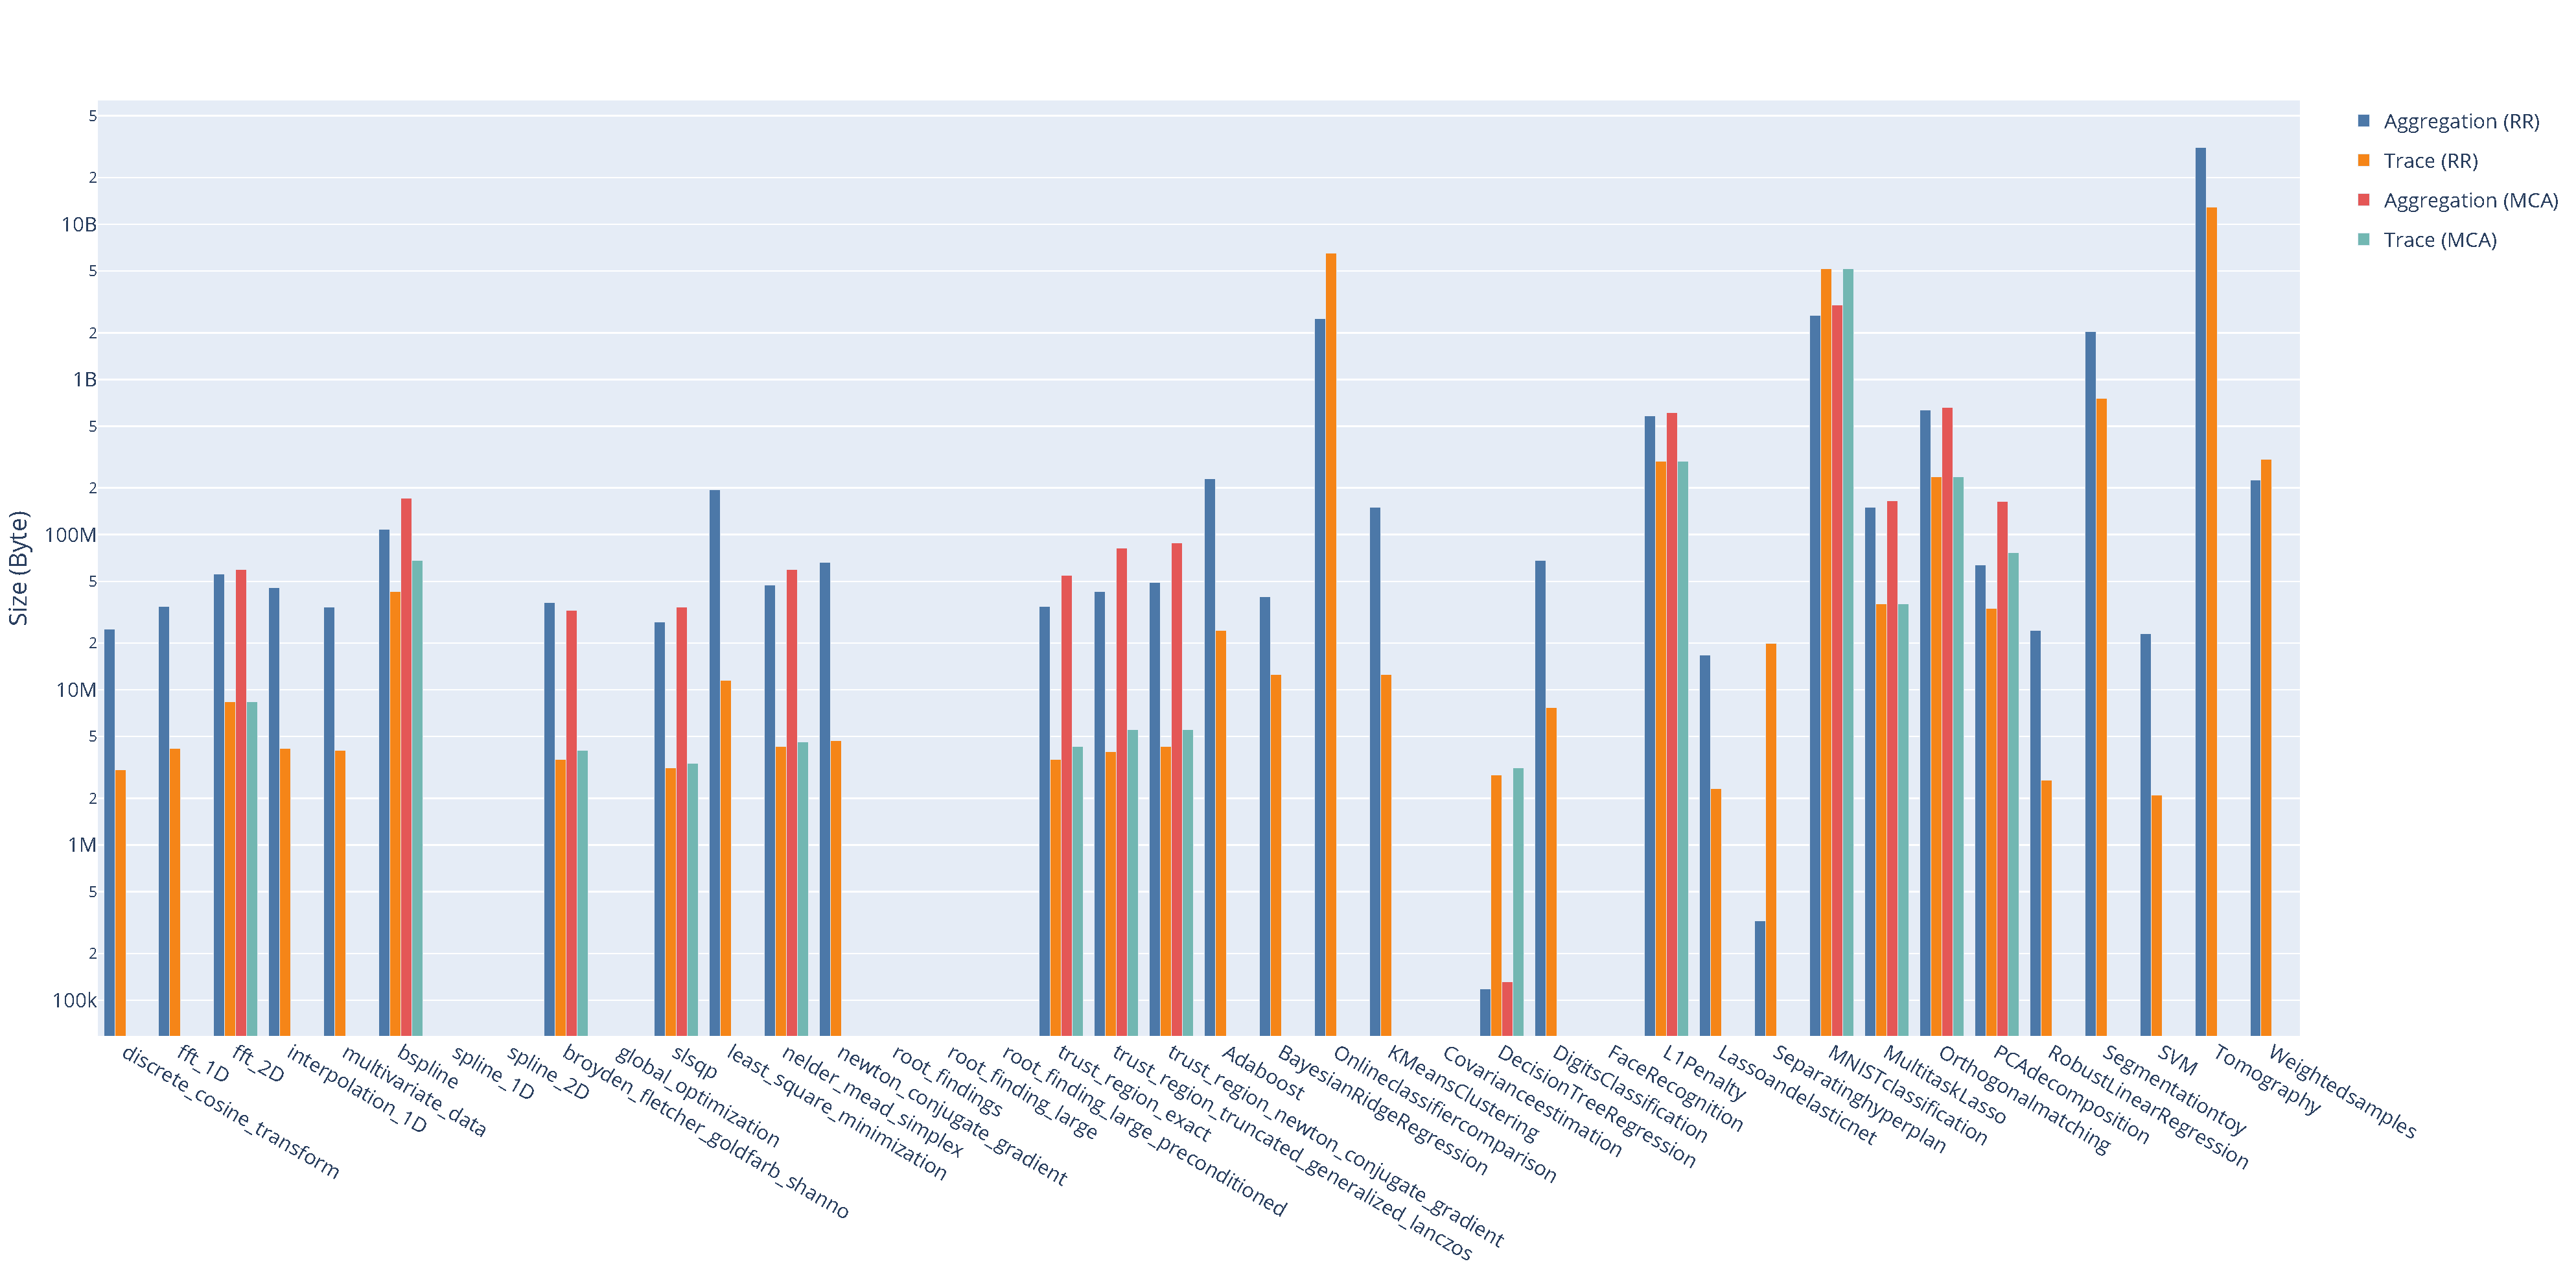
\includegraphics[width=\linewidth]{figure/parsing.pdf}
    \caption{\pytracer trace and aggregation files size.
    The figure presents the size measured for the trace and the aggregation size files.}
    \label{fig:performance_parsing_size}
\end{figure}


\begin{table}
\centering
\begin{subfigure}[t]{.75\linewidth}
    \centering
    \begin{tabular}{|l|c|c|c|c|}
    \hline 
    Application & Original & Pytracer only & RR & MCA \\
    \hline 
    Loading & 0.456 & 8.152 & - & - \\
    \hline
    discrete\_cosine\_transform & 0.280 & 8.176 & 10.203 & - \\ 
    fft\_1D & 0.650 & 9.075 & 11.345 & - \\
    fft\_2D & 0.311 & 9.500 & 11.929  & 16.433   \\
    \hline
    interpolation\_1D & 0.377 & 8.803  & 11.954  & -   \\
    multivariate\_data &0.626 & 8.648 &  12.711  & - \\
    bspline & 0.109  & 9.050 & 13.396  & 16.830   \\
    spline\_1D & 0.111 & 8.618 & 10.960   & - \\
    spline\_2D & 0.655 & 8.649 & 19.424  & - \\
    \hline
    broyden\_fletcher\_goldfarb\_shanno &0.475 & 8.292 & 11.033 & 13.685 \\
    global\_optimization &1.257 & 55.916  & 93.322  & - \\
    slsqp & 0.469 & 8.192 & 10.795 & 12.439  \\
    least\_square\_minimization & 0.505 & 10.151  & 13.888 & -  \\
    nelder\_mead\_simplex & 0.471 & 8.418  & 11.382  & 12.792  \\
    newton\_conjugate\_gradient & 0.487 & 8.548  & 11.956  & 14.281 \\
    root\_findings & 0.462 & 8.198  & 10.787   & - \\
    root\_finding\_large & 0.801 & 11.525 & 41.493   &  82.701  \\
    root\_finding\_large\_preconditioned & 0.702 & 10.580 & 33.199   & 57.579  \\
    trust\_region\_exact & 0.482 & 8.170 & 10.400  & 12.524 \\
    trust\_region\_truncated\_generalized\_lanczos & 0.459 & 8.457 & 11.216 & 13.245  \\
    trust\_region\_newton\_conjugate\_gradient & 0.479 & 8.538 & 11.179 & 13.488 \\
    \hline
    Adaboost &1.388 &14.553 &  20.999 & - \\
    Bayesian Ridge Regression & 1.086 & 10.344 & 90.299 & -  \\
    Online classifier comparison & 15.964 & 72.691 & 2104.114 & -  \\
    K-Means Clustering & 1.621 & 17.614  & 34.005 & 52.902   \\
    Covariance estimation & 1.357 & 11.755 & 23.964  & -   \\
    Decision Tree Regression & 1.185 & 11.194 & 15.760 & 15.918  \\
    Digits Classification & 1.672 & 12.725 & 40.634 & - \\
    Face Recognition & 32.159  & 74.356 & - & - \\
    L1 Penalty & 1.568 & 12.591 & 65.547 & 128.220 \\
    Lasso and elastic net & 1.057 & 9.903 & 17.078 & -  \\
    Separating hyperplan & 1.376 & 11.532  & 22.333 & 25.036 \\
    MNIST classification & 19.650 & 37.838 & 402.389  & - \\
    Multitask Lasso & 1.090 &10.196 & 15.025  & - \\
    Orthogonal matching & 1.161 & 12.129 & 21.779   & 31.135 \\
    PCA decomposition & 1.239 & 10.642 & 15.520 & 17.952    \\
    Robust Linear Regression & 1.370 & 11.144  & 14.280  & - \\
    Segmentation toy &1.679 & 22.385 & 87.811  & - \\
    SVM & 1.403 & 11.737 & 23.203 & 24.126   \\
    Tomography & 11.108 & 40.177  & 1376.134 & -  \\
    Weighted samples & 1.358 & 11.768 & 21.255 & 20.541   \\
    \hline
    \end{tabular}
\end{subfigure}
    \caption{\pytracer tracing performances.}
    \label{tab:pytracer_overhead}
\end{table}

    
% \begin{table}[]
%     \centering
%     \begin{tabular}{c|c|c|c|c}
%          Pytracer & Verificarlo Instrumentation & Backend & Time (hours:minutes:seconds) & Overhead \\
%          \hline 
%          No & No & - & 00:30:51 & 1 \\
%          No & Yes & IEEE & 01:32:56 & 3 \\
%          No & Yes & RR & 16:52:08 & 32 \\
%          Yes & No & - & 03:11:07 & 6  \\
%          Yes & Yes & IEEE & 11:14:33 & 22 \\
%          Yes & Yes & RR & 25:05:54 & 48 \\
%     \end{tabular}
%     \caption{Overheads of \pytracer on PyAFQ experiment with and without fuzzy.}
%     \label{tab:pytracer_overhead}
% \end{table}

% \begin{table}[]
%     \centering
%     \begin{tabular}{c|c|c|c|c}
%          Pytracer & Verificarlo Instrumentation & Backend & Time (hours:minutes:seconds) & Overhead \\
%          \hline 
%          No & No & - & 15 & 1 \\
%          No & Yes & IEEE & 49 & 3 \\
%          No & Yes & RR &  & 441 & 29 \\
%          Yes & No & - & 03:11:07 & 6  \\
%          Yes & Yes & IEEE & 11:14:33 & 22 \\
%          Yes & Yes & RR & 25:05:54 & 48 \\
%     \end{tabular}
%     \caption{Caption}
%     \label{tab:pytracer_overhead}
% \end{table}

\subsection{Postprocessing}

The figures~\ref{fig:performance_parsing_time} and~\ref{fig:performance_parsing_size} show
the postprocessing time and trace's sizes produced by \pytracer.
We only report time for parsing and aggregation that have been successful.
We measure a throughput of 7MB/s by taking the ratio size over time. 
Finally, \pytracer has been tested on PyAFQ~\cite{kruper2021evaluating}, a neuroimaging Python tool
to automated fiber quantification with generated traces of 
1TB that \pytracer was able to handle and fluently visualize.


\section{Discussion}

\pytracer is a tool for visualizing the numerical quality of function inputs/outputs over time.
It generates numerical traces that are aggregated in postprocessing to measure numerical discrepancies between executions.
\pytracer does not make any assumption about the noise model used to estimate uncertainties but has been tested with the MCA 
through the fuzzy ecosystem on two broadly used scientific libraries for Python with partial success.

As we showed in section~\ref{sec:impact_mca_modes}, using the Full MCA mode leads to runtime errors that have a considerable impact on the proper functioning of the execution, which is unfortunate since these
errors do not reflect actual numerical errors but errors related to perturbations that should not occur.
Fixing this misbehavior would greatly help use Full MCA mode since this mode allows simulating catastrophic cancellations, which are familiar sources of numerical errors. By preserving exact operations, RR mode is far more conservative and so easy to use even though it does not simulate all perturbations that might be encountered.

Also, using a post-process analysis to aggregate traces, \pytracer falls in the same pitfalls as veritracer and is limited to aggregate traces where the execution flow path extremely diverges. Therefore, a posteriori reconstruction
is a challenging task as one must precisely identify the flow path taken and find synchronization points to pursue the analysis. We retrieve, for example, this divergence behavior in two general classes of numerical schemes: iterative methods and optimization processes. One solution to overcome this issue is to integrate methods used in code coverage analysis to keep track of flow paths taken and the backtraces.
However, this would increase the complexity of the postprocess analysis as well as an extra slowdown factor.
However, we believe that by coupling the Gantt chart with static analysis, \pytracer would catch some divergence patterns occurring within a function. Indeed, by instrumenting at the function level, \pytracer has a view on function's callees (i.e., the functions called within a function) and thus should partially detect flow divergences.

By design principle, \pytracer is flexible on the noise model used, although we only test it with the MCA model in our experiments.
Nevertheless, we would like to compare different models against MCA in future works to see the resulting differences. 
In particular, although \pytracer only works on a sequential application for the moment, it can be used to analyze parallel sections internal to a function.
The only restriction is that the section does not call other functions traced by \pytracer; we would fall into the previous issue of divergence if it would not be the case.
Since \pytracer only cares about inputs and outputs of a function, the order of internal operations is transparent for it and thus should be able to handle those cases.

Finally, \pytracer does not instrument elementary arithmetic operations, and it can be a barrier to more profound analysis.
However, we believe that instrumentation at the function level presents two advantages: it first limits the size of the traces since only inputs and outputs of a function are dumped instead of a full report which, on the one hand, decrease the overhead of the instrumentation and, on the other hand, help the user to identify instabilities quickly. One of the pitfalls can be overwhelming the user with too much information, which makes analysis more difficult. Nevertheless, the analysis at fine granularity can be interesting at the final step of the understanding. Such an analysis would require a different instrumentation approach by, for example, working at the Abstract Syntax Tree (AST) level since it is trivial to get it in Python.
An ideal way to do that would be to be able to extract and replay a function, in the same vein as the CERE~\cite{castro2015cere} tool does but for Python, and use an AST instrumentation to analyze step by step 
the numerical quality of elementary operations within the fuzzy environment.
Lastly, AST analysis can serve as a basis for finding relationships between variables, which is valuable information for the user.

In addition to runtime errors that it raises, mismatching shapes is also a problem when aggregating traces as \pytracer will not compute statistics for a set of arrays having different shapes.
Two solutions exist to overcome this issue: the first one is to not instrument the \texttt{PyArray\_Arange} function with MCA. The advantage is that it is easy to set up since it requires one extra line in the exclusion file.
However, the same kind of problem may appear somewhere else
because, as we have seen, the operations being evolved are elementary. The chances that developers reproduce the same pattern are very probable. The second solution is to ensure that the Full MCA mode preserves the exact operations.
This solution has the advantage of not worrying about which functions should be instrumented or not with MCA, but it is hard to achieve it in practice. Indeed, we rely on the MCA implementation provided by Verificarlo that uses an internal precision to add the random perturbation that is higher than the working precision for applying the random noise. Verificarlo then rounds the result to the working precision before returning it, so any residual noise lower than the working precision is lost. 
Keeping track of that noise would require recording each intermediate computation in a shadow memory or keeping a tag about their exactness.
\Yohan{This idea has emerged by discussing with Verificarlo's team. 
I must find a way to express that and not give the impression that we discovered or suggest it.}
This option would require more extra works than the first one but would ensure more consistent results.

\section{Conclusion}


% \tristan{I moved this from the opening of Section 4, as this reads more like a summary of \pytracer's features than an experiment description. It should be refactored in 1-2 paragraphs summarizing the main properties of \pytracer.}

\pytracer is the first tool to propose a complete framework
for analyzing and visualizing the numerical stability of Python codes.
It works by automatically instrumenting Python libraries to produce numerical
traces that can be interactively visualized through a Dash server.
\pytracer does not require a manual intervention from the user neither rely on
specific libraries and has been tested successfully tested on 
intensively used on scientific libraries such as NumPy, SciPy and Scikit-learn. We demonstrated on a set of representative tests that \pytracer is scalable with an average instrumentation slowdown of $times 3.5$ and that is can handle traces up to 1TB while offering a fluent visualization to the user. Moreover,
\pytracer is by construction agnostic to the noise model used 
to evaluate the numerical stability. We demonstrated 
that \pytracer can be used with the Monte Carlo Arithmetic 
through the fuzzy environment. 
The experiments conducted in this paper are the first largest application of the fuzzy ecosystem by the wide range of applications covered. It is also the occasion for us to
provided  feedback 
about pitfalls and benefits encountered
in order to shed light on the good and bad practices for first-time users and democratize MCA's usage.
\pytracer is available at \href{https://github.com/yohanchatelain/pytracer}{github://yohanchatelain/pytracer} under an open source licence.

% \begin{itemize}

%     \item Domain agnostic: \pytracer is intended to work on any scientific Python applications, without specific domain-specific languages or needs to rely on specific libraries.
%     We target two of the most common libraries used in scientific computing within Python, SciPy and Scikit-learn, and a domain-specific application in neuroimaging. We show that \pytracer works well on these libraries, capturing most of the functions' module targeted.

%     \item Automatic: \pytracer objective is to offer automatic instrumentation for Python applications,
%     from small prototypes to state-of-the-art scientific libraries. 

%     \item Scalable: \pytracer goal is to trace real-world application and use case.
%     In that perspective, we use \pytracer on PyAFQ, a domain-specific neuroimaging application to compute tractograms, generating \pytracer traces up to 1TB. We demonstrate that \pytracer can handle this volume of data and offer the user an interactive and fluent visualization.
%     We also show that \pytracer instrumentation gives a slowdown of $\times 6$.

%     \item Fuzzy compatible: \pytracer aims at evaluating numerical stability by using an injection noise model.
%     Although the noise model used is orthogonal to \pytracer tracing mechanism, we emphasize in these experiments the MCA model through the fuzzy environment and discuss its compatibility with \pytracer tracing mechanism to point out limitations of the trace-based approach and to propose research tracks to overcome them.
%     The experiments conducted in this paper are the first largest application of the fuzzy ecosystem by the wide range of applications covered. We, therefore, found it interesting to give feedback about pitfalls and benefits encountered
%     in order to shed light on the good and bad practices for first-time users and democratize MCA's usage.
%     Moreover, these analyses will help the fuzzy developers to increase the overall stability of fuzzy.

% \end{itemize}

\bibliographystyle{abbrv}
\bibliography{biblio}

%%
%% If your work has an appendix, this is the place to put it.
\appendix

\end{document}
\endinput
%%
%% End of file `sample-authordraft.tex'.
